\chapter{Partial kernels and quotient equilibrium}
\label{chap:partial-bergman}

\begingroup
\predisplaypenalty=10000

Throughout this chapter, $L$ is a holomorphic line bundle on $X$ with a smooth Hermitian metric $h$. In a local holomorphic frame $e$ write $|e|_h^2=\mathrm{e}^{-\chi}$; the curvature form $c_1(L,h)=\ddc\chi$ is a smooth closed real $(1,1)$-form, independent of the frame, as in \cref{chap:sections}.

A quasi-plurisubharmonic function $\varphi$ on $X$, the selecting potential, selects in each tensor power $L^m$ the holomorphic sections $s$ for which $|s|_{h^m}^2\mathrm{e}^{-m\varphi}$ is locally integrable. A partial Bergman kernel is the Bergman kernel of this space of sections for a Hilbert norm defined by a continuous weight: the singular function $\varphi$ decides which sections occur, but it does not enter their norms. On a compact K\"ahler manifold, if $\varphi$ is $c_1(L,h)$-plurisubharmonic with positive non-pluripolar Monge--Amp\`ere mass, the normalized kernel measures converge to the Monge--Amp\`ere measure of a partial envelope. This envelope is the largest $c_1(L,h)$-plurisubharmonic function that is at least as singular as $\varphi$ in the sense of multiplier ideals and lies below the continuous weight on the set where the norm is computed. This chapter studies how much of this equilibrium theory survives when $X$ is not K\"ahler, and when the selecting potential is plurisubharmonic only with respect to a Hermitian form unrelated to the curvature of $L$.

One direction of the K\"ahler argument is local and works on every compact complex manifold. A Bernstein--Markov estimate, which follows from the submean inequality, keeps the partial Fubini--Study potentials below the weight, and Lelong-number estimates on local modifications keep their limits at least as singular as $\varphi$ in the sense of multiplier ideals. Together these bound every limit of the potentials by the partial envelope. A matching lower bound requires global sections approximating the envelope, and this is where the K\"ahler hypothesis enters. If $X$ admits a modification from a compact K\"ahler manifold, the relative canonical bundle with a Jacobian metric makes the selected spaces upstairs and downstairs isometric, and the K\"ahler theorem gives convergence of the kernel measures on $X$ itself.

Fibrations show what can happen without such a modification. On a holomorphic submersion with compact connected fibers, every section of a pulled-back line bundle is constant along the fibers and descends to the base. Probability measures on the fibers make this descent an isometry, so the kernel measures on the total space are lifts of kernel measures on the base. Their limit, the quotient equilibrium measure, is the lift of the equilibrium measure of the base, and it appears at the growth rate $m^{\dim B}$ of the section spaces rather than at $m^{\dim X}$. On the Hopf manifold it is a Hermitian Monge--Amp\`ere measure; in dimension three this gives a nonzero limit on a manifold without the bounded mass property.

A selecting potential that is plurisubharmonic only with respect to a Hermitian form need not descend, but the sections it selects still do, so its singularities act only through a vanishing condition on the base. For isolated logarithmic poles, for poles along a section over a base divisor, and for anisotropic singularities controlled by integrability along the fibers, this condition differs from a multiplier-ideal condition on the base by a bounded number of vanishing orders. Such shifts cost only $O(m^{\dim B-1})$ sections, and for point poles and for poles along a section over a divisor the kernel measures still converge to a quotient equilibrium measure. The price is a loss of information: moving a pole along its fiber changes the multiplier ideals on $X$ but leaves every kernel unchanged. Explicit point and divisor models on projective bases compute the limits through binomial tails, and a change of the integration volume separates the base equilibrium measure from the conditional fiber probabilities carried by its lift.

The remaining sections study explicit selections for which the kernel asymptotics can be computed directly. When vanishing orders grow sublinearly in $m$, an entire-function model gives a Gaussian transition on a shrinking scale; a uniform local norm comparison and a global $L^2$ correction show how far this transition persists on a compact curve. In two dimensions, competing monomials at a fixed zero of the curvature produce a logarithmic factor in the kernel scale, which an explicit metric on $\mathbb P^2$ makes computable. A Newton polytope selects monomials directly: its logarithmic growth constraint determines the envelope, while lattice counting and concentration of the monomial norms determine the measure limit. For a lower-dimensional polytope this limit is a positive measure carried by real tori, although the higher curvature powers of the envelope vanish. Finally, multiplier ideals need not form a graded series of section spaces. At critical divisors, rounding can make the leading section count oscillate between even and odd degrees, while at the two base points of a pencil three neighboring bands of monomials contribute to a single positive limit.

We use the following notation from earlier chapters. For quasi-plurisubharmonic functions $u,v$, we write $u\preceq v$ if $u\leq v+C$ for a constant $C$, and $u\sim v$ if $u\preceq v\preceq u$ (\cref{def:singularity-order}); we write $u\preceq_{\mathcal I}v$ if $\mathcal I(ku)\subseteq\mathcal I(kv)$ for every real $k>0$, and $u\sim_{\mathcal I}v$ if these ideals are equal for every $k>0$ (\cref{sec:psh-singularity-types}). For a smooth real $(1,1)$-form $\theta$, $P_\theta[u]_{\mathcal I}$ is the multiplier-ideal envelope of \cref{def:hermitian-i-envelope}, and $V_\theta$ is the upper envelope of all nonpositive $\theta$-plurisubharmonic functions, which has minimal singularities (\cref{sec:obstacle-envelopes}). The non-pluripolar Monge--Amp\`ere measure of $u\in\PSH(X,\theta)$ is written $\mathrm{MA}_\theta(u)$, or $\mathrm{MA}^{\mathrm{ext}}_\theta(u)$ when its mass may be infinite (\cref{thm:arbitrary-extended-ma}).

\section{Selected spaces and partial Bergman kernels}\label{sec:partial-selected-space}\index{Bergman kernel!partial}

Fix a quasi-plurisubharmonic function $\varphi$ on $X$, the \emph{selecting potential}, and a smooth positive probability measure $\nu$ on $X$. For each integer $m\geq1$, the \emph{selected space}\index{Selected space} of degree $m$ and its dimension are
\[
 V_m=H^0\bigl(X,L^m\otimes\mathcal I(m\varphi)\bigr),
 \qquad N_m=\dim V_m.
\]
Instead of $\varphi$, the Hilbert norm on $V_m$ uses a real continuous weight $v\in C(X)$:
\[
 \|s\|_{m,v,\nu}^2=\int_X|s|_{h^m}^2\mathrm{e}^{-mv}\,\mathrm{d}\nu
 \quad(s\in V_m).
\]
Since $v$ is bounded, this integral is finite for every global section. It vanishes only for $s=0$, because $\nu$ has a positive density and a holomorphic section vanishing almost everywhere vanishes identically. This separation of the selecting potential from the norm follows \cite[Section~14.3]{SGPT}.

\Needspace{13\baselineskip}
Fix also an integer $r\geq1$, which determines the normalization below; it will be chosen as the growth degree of $N_m$, which may be smaller than $n$. Let $s_1,\ldots,s_{N_m}$ be an orthonormal basis of $V_m$ for the norm $\|\cdot\|_{m,v,\nu}$. The \emph{partial Bergman kernel} and the \emph{partial kernel measure} are
\[
 B_{m,v,\varphi,\nu}(x)
       =\mathrm{e}^{-mv(x)}\sum_j|s_j(x)|_{h^m}^2
 \quad(x\in X),
 \qquad
 \beta_m^{(r)}=\frac{r!}{m^r}B_{m,v,\varphi,\nu}\,\nu.
\]
By unitary invariance they do not depend on the orthonormal basis, and both are zero when $V_m=\{0\}$. The evaluation argument of \cref{prop:finite-bergman-identities} gives the extremal formula and the total mass:
\[
 B_{m,v,\varphi,\nu}(x)
 =\sup_{\substack{s\in V_m\\\|s\|_{m,v,\nu}\leq1}}
       |s(x)|_{h^m}^2\mathrm{e}^{-mv(x)},
 \qquad
 \int_X\beta_m^{(r)}=\frac{r!N_m}{m^r}.
\]
The selecting potential enters only through $V_m$. In particular, for fixed $h$, $v$ and $\nu$, if the multiplier ideals $\mathcal I(m\varphi)$ are contained in those of another selecting potential, then so are the selected spaces, and the extremal formula shows that the kernels are ordered in the same way.

Replacing $h$ by $h\mathrm{e}^{-a}$ and $v$ by $v-a$, for a smooth real function $a$, leaves $h^m\mathrm{e}^{-mv}$, and hence the norm and the kernel measure, unchanged.

\section{A local Bernstein--Markov estimate}
\label{sec:partial-bernstein-markov}

A Bernstein--Markov estimate compares the supremum norm of sections on a weighted compact set with an integral norm, up to an exponential loss in the degree whose rate can be made arbitrarily small. It is what keeps partial Fubini--Study potentials below the weight in the limit. For a smooth positive volume and a continuous weight on the whole manifold, it follows from the submean inequality.

For a compact set $K\subseteq X$ and $w\in C(K)$, write
\[
 \|s\|_{m,w,K}=\sup_K |s|_{h^m}\mathrm{e}^{-mw/2}.
\]
A probability measure $\mu$ on $K$ is \emph{Bernstein--Markov} for $(K,w)$ if, for every $\epsilon>0$, there is a constant $C_\epsilon$ such that
\[
 \|s\|_{m,w,K}\leq C_\epsilon \mathrm{e}^{\epsilon m}
          \left(\int_K|s|_{h^m}^2\mathrm{e}^{-mw}\,\mathrm{d}\mu\right)^{1/2}
\]
for all $m\geq1$ and all $s\in H^0(X,L^m)$. If $K$ is non-pluripolar, the supremum norm is a norm: the zero set of a nonzero section is an analytic hypersurface, hence pluripolar, and cannot contain $K$. The Bernstein--Markov inequality then shows that the integral
\[
 \|s\|_{m,w,\mu}^2=\int_K|s|_{h^m}^2\mathrm{e}^{-mw}\,\mathrm{d}\mu
\]
is also a norm on $H^0(X,L^m)$, and in particular on every selected space $V_m$. The definitions of \cref{sec:partial-selected-space} therefore apply with $(X,v,\nu)$ replaced by $(K,w,\mu)$. We write $B_{m,w,\varphi,\mu}$ for the resulting partial Bergman kernel on $K$ and $\beta_m^{(r)}=(r!/m^r)B_{m,w,\varphi,\mu}\,\mu$ for the partial kernel measure; the extremal formula and the total mass $r!N_m/m^r$ hold as before.

\begin{proposition}\label{prop:hermitian-full-bm}\index{Bernstein--Markov estimate}
Let $v\in C(X)$. Every smooth positive probability measure on $X$ is Bernstein--Markov for $(X,v)$.
\end{proposition}
\begin{proof}
Let $\nu$ be a smooth positive probability measure, and fix $\epsilon>0$. Cover $X$ by finitely many coordinate charts on which $L$ has holomorphic frames, and choose relatively compact open subsets of these charts that still cover $X$. In a frame $e$ write $|e|_h^2=\mathrm{e}^{-\chi}$ and $s=f e^{\otimes m}$, so that $|s|_{h^m}^2\mathrm{e}^{-mv}=|f|^2\mathrm{e}^{-m(\chi+v)}$. By compactness and uniform continuity of the finitely many functions $\chi+v$, there is a radius $\delta>0$ with the following property: every point $x$ lies in one of the smaller sets, the coordinate ball $B(x,\delta)$ lies in the corresponding chart, and the oscillation of $\chi+v$ on $B(x,\delta)$ is at most $2\epsilon$. On these balls the density of $\nu$ with respect to coordinate Lebesgue measure is bounded below by a positive constant independent of $x$.

\Needspace{8\baselineskip}
The submean inequality for the holomorphic function $f$ on $B(x,\delta)$ therefore gives
\[
 \begin{split}
 |s(x)|_{h^m}^2\mathrm{e}^{-mv(x)}
 &=|f(x)|^2\mathrm{e}^{-m(\chi+v)(x)}\\
 &\leq C_\delta \mathrm{e}^{2\epsilon m}
                 \int_{B(x,\delta)}|f|^2\mathrm{e}^{-m(\chi+v)}\,\mathrm{d}\nu\\
 &\leq C_\delta \mathrm{e}^{2\epsilon m}\|s\|_{m,v,\nu}^2,
 \end{split}
\]
with $C_\delta$ independent of $x$ and $m$. Taking the supremum over $x$ and then the square root gives the Bernstein--Markov inequality with $C_\epsilon=C_\delta^{1/2}$.
\end{proof}

For a general compact set $K$ and weight $w\in C(K)$, the Bernstein--Markov property is not automatic, and we assume it explicitly whenever it is needed.

\section{Partial envelopes on a weighted compact set}
\label{sec:hermitian-partial-envelopes}

A continuous obstacle on a non-pluripolar compact set bounds all admissible potentials globally. Imposing a multiplier-ideal constraint then fixes the ordinary singularity type of the envelope: it agrees with the normalized ideal envelope up to bounded functions.

Let $\theta$ be a smooth real $(1,1)$-form on $X$, let $\varphi\in\PSH(X,\theta)$, let $K\subseteq X$ be compact and non-pluripolar, and let $w\in C(K,\mathbb R)$. Use the multiplier-ideal order characterized in \cref{thm:local-i-inputs} and the quasi-everywhere convention of \cref{sec:obstacle-envelopes}. Define
\begin{equation}\label{eq:hermitian-partial-i-envelope}
 \begin{aligned}
 E_{\theta,K}[\varphi]_{\mathcal I}(w)
 &=\Bigl(\sup\bigl\{a\in\PSH(X,\theta):
       a\preceq_{\mathcal I}\varphi,\\
 &\hspace{52pt}a\leq w\text{ quasi-everywhere on }K\bigr\}\Bigr)^*.
 \end{aligned}
\end{equation}

\begin{theorem}\label{thm:hermitian-partial-i-envelope}
The function $E=E_{\theta,K}[\varphi]_{\mathcal I}(w)$ is a genuine $\theta$-plurisubharmonic function and the largest member of its defining family. Let $q=P_\theta[\varphi]_{\mathcal I}$, and let $C$ be any upper bound from \cref{lem:compact-obstacle-upper-bound}. Then
\[
 q+\min_Kw\leq E\leq q+C.
\]
In particular, $E$ has the ordinary singularity type of $q$, and
\[
 E\sim_{\mathcal I}\varphi.
\]
\end{theorem}
\begin{proof}
\Cref{thm:hermitian-i-projection} gives $q\leq0$ and $q\sim_{\mathcal I}\varphi$. Thus $q+\min_Kw$ belongs to the defining family. \Cref{lem:compact-obstacle-upper-bound} bounds the entire family above by $C$, so its regularized supremum is genuine and gives the lower inequality.

For each competitor $a$, the upper bound $\sup_Xa\leq C$ and \cref{prop:p-below-i,prop:i-envelope-operations} give
\[
 a-C\leq a-\sup_Xa\leq P_\theta[a]_{\mathcal I}
                    \leq P_\theta[\varphi]_{\mathcal I}=q.
\]
Taking regularized suprema proves $E\leq q+C$.

The two bounds show that $E$ and $q$ differ by a bounded amount. They therefore have the same multiplier ideals, and these equal those of $\varphi$.

It remains to check the obstacle after regularization. Choose a countable subfamily by Choquet's lemma, and replace it by successive finite maxima. Finite maxima remain admissible, by \cref{thm:local-i-inputs} and by taking the finite union of the obstacle's exceptional sets. Let $a_j$ be the resulting increasing sequence. Outside a countable union of pluripolar subsets of $K$, every $a_j$ is at most $w$. The unregularized limit is therefore at most $w$ there. The regularized limit equals $E$ and changes this limit only on a further pluripolar set, by the local supremum theorem in \cref{sec:obstacle-envelopes}. Thus $E\leq w$ quasi-everywhere on $K$.

We have proved that $E$ is a member of its defining family. It dominates each competitor by construction, so it is the largest member; in particular the unregularized supremum in \eqref{eq:hermitian-partial-i-envelope} already equals $E$ at every point.
\end{proof}

\Needspace{25\baselineskip}
\begin{proposition}\label{prop:partial-envelope-calculus}
The envelope depends only on the multiplier-ideal class of $\varphi$. It is increasing in the obstacle and in the multiplier-ideal order of $\varphi$. For $w,w'\in C(K)$ and $c\in\mathbb R$,
\[
 \begin{split}
 E_{\theta,K}[\varphi]_{\mathcal I}(w+c)
       &=E_{\theta,K}[\varphi]_{\mathcal I}(w)+c,\\
 \bigl|E_{\theta,K}[\varphi]_{\mathcal I}(w)
       -E_{\theta,K}[\varphi]_{\mathcal I}(w')\bigr|
       &\leq\|w-w'\|_{C(K)}.
 \end{split}
\]
The second line means the two corresponding pointwise inequalities, including at poles. For $0<t<1$, smooth real $(1,1)$-backgrounds $\theta_i$ on $X$, for $i=0,1$, potentials $\varphi_i\in\PSH(X,\theta_i)$ and obstacles $w_i\in C(K)$, put $\theta_t=(1-t)\theta_0+t\theta_1$, and similarly define $\varphi_t,w_t$. Then
\[
 (1-t)E_{\theta_0,K}[\varphi_0]_{\mathcal I}(w_0)
       +tE_{\theta_1,K}[\varphi_1]_{\mathcal I}(w_1)
 \leq E_{\theta_t,K}[\varphi_t]_{\mathcal I}(w_t).
\]
For a smooth real $f$, changing the background and obstacle gives the exact identity
\[
 E_{\theta+\ddc f,K}[\varphi-f]_{\mathcal I}(w-f|_K)
       =E_{\theta,K}[\varphi]_{\mathcal I}(w)-f.
\]
\end{proposition}
\begin{proof}
Equality or inclusion of the defining families proves the first two assertions. Adding a constant gives a bijection of competitor families, proving translation. Apply monotonicity to $w'\pm\|w-w'\|_{C(K)}$ to obtain the two inequalities in the second line.

For concavity, the left side is $\theta_t$-plurisubharmonic and obeys the obstacle $w_t$ outside the union of two pluripolar exceptional sets. Each of its summands has the multiplier-ideal class of its prescribed singularity by the theorem. Addition and positive scaling in \cref{lem:hermitian-i-calculus} give the multiplier-ideal class of $\varphi_t$. Thus the left side is an admissible competitor on the right. Finally, $a\mapsto a-f$ is a bijection of the two families in the gauge identity, and regularization commutes with subtraction of a smooth function.
\end{proof}

The envelope bounds candidate limits of the partial Fubini--Study potentials. The next argument proves this upper bound; identifying a kernel measure with its Monge--Amp\`ere measure will require the geometric convergence hypotheses developed afterward.


\section{An upper bound for partial Fubini--Study limits}
\label{sec:partial-kernel-upper}

There is also an asymptotic statement that does not require a K\"ahler manifold or positive Monge--Amp\`ere mass. It gives the upper bound for the potentials associated with partial kernels. Obtaining the reverse inequality is a separate generation problem.

Let $X$ be a connected compact complex manifold of dimension $n\geq1$, and let $L\to X$ be a holomorphic line bundle with smooth Hermitian metric $h$ and curvature $\theta=c_1(L,h)$. Assume $\varphi\in\PSH(X,\theta)$. Fix a closed non-pluripolar set $K$, a continuous real weight $w$ on $K$, and a Bernstein--Markov probability measure $\mu$ for $(K,w)$. For each positive integer $m$, set $V_m=H^0(X,L^m\otimes\mathcal I(m\varphi))$ and $N_m=\dim V_m$. Choose an orthonormal basis $s_1,\ldots,s_{N_m}$ for the continuous weighted norm of \cref{sec:partial-bernstein-markov}, and define the global partial Fubini--Study potential
\[
 U_m=\frac1m\log\sum_{j=1}^{N_m}|s_j|_{h^m}^2
 \quad(N_m>0).
\]
Set $U_m=-\infty$ if $N_m=0$. For a nonempty space the local expression in a frame shows that $U_m\in\PSH(X,\theta)$ and has analytic singularity type. On $K$, it satisfies $\mathrm{e}^{m(U_m-w)}=B_{m,w,\varphi,\mu}$.

\begin{lemma}\label{lem:ideal-modification-lelong-loss}
Let $U\subseteq X$ be open, and let $\pi:Y\to U$ be a local modification with smooth source, let $y\in Y$, and let $J_\pi$ be its holomorphic Jacobian in coordinates near $y$. If a nonzero holomorphic germ $g$ belongs to $\mathcal I(m\varphi)$ on $U$, then
\[
 \operatorname{ord}_y(g\circ\pi)
       \geq m\nu(\varphi\circ\pi,y)-n-\operatorname{ord}_yJ_\pi.
\]
Consequently, for every nonempty $V_m$,
\[
 \nu(U_m\circ\pi,y)
       \geq\nu(\varphi\circ\pi,y)
                   -\frac{n+\operatorname{ord}_yJ_\pi}{m}.
\]
\end{lemma}
\begin{proof}
If $n\geq2$, let $\rho:\widetilde Y\to Y$ be the blowup of $y$ and let $E$ be its exceptional divisor. For $n=1$, take $\rho$ to be the identity and $E=\{y\}$. Set $F=\pi\circ\rho$ and write $J_F$ for its local holomorphic Jacobian determinant. Generic orders along $E$ give
\[
 \nu(\varphi\circ F,E)=\nu(\varphi\circ\pi,y),\qquad
 \operatorname{ord}_E(g\circ F)=\operatorname{ord}_y(g\circ\pi).
\]
On a standard blowup chart the Jacobian of $\rho$ has order $n-1$ along $E$. The chain rule therefore gives the log discrepancy over $U$ as
\[
 A_U(E)=1+\operatorname{ord}_E J_F
       =n+\operatorname{ord}_yJ_\pi.
\]
Since $g\in\mathcal I(m\varphi)$, its order along $E$ is at least the order of this ideal. The lower estimate in \cref{lem:bergman-divisorial-error}, applied to $F$, now proves the first assertion.

For the second, write each basis section in a local frame. The Lelong number of the logarithm of a sum of squared holomorphic functions is the minimum of their orders in the convention of this book. The pulled-back smooth metric has zero Lelong number, so dividing by $m$ gives the result.
\end{proof}

We shall use the local version of \cref{lem:modification-lone-pullback}. Namely, $L^1_{\loc}$ convergence of potentials with a common smooth curvature lower bound is preserved under a fixed smooth local modification. Here is the same proof in its local form. On relatively compact subsets the pullbacks are locally bounded above and have a common smooth lower curvature bound. After smooth correction, local plurisubharmonic compactness supplies subsequential limits or collapse to $-\infty$ on a connected coordinate region. Every such region meets the complement of the exceptional locus. There the modification is a biholomorphism, and change of variables gives $L^1_{\loc}$ convergence to the expected pullback. Collapse is therefore excluded. Every subsequential limit equals that pullback off the exceptional locus, hence almost everywhere and then as its canonical representative. Uniqueness of cluster limits gives convergence along the whole sequence.

\begin{theorem}\label{thm:partial-fubini-study-upper}
Along the indices for which $N_m>0$, the potentials $U_m$ form a relatively compact family in $L^1(X)$. Every cluster limit $U$ along indices tending to infinity is genuine, has multiplier-ideal order
\[
 U\preceq_{\mathcal I}\varphi,
\]
and satisfies $U\leq w$ quasi-everywhere on $K$. Consequently
\[
 \left(\limsup_{m\to\infty}U_m\right)^*
       \leq E_{\theta,K}[\varphi]_{\mathcal I}(w).
\]
If only finitely many spaces are nonempty, the last left side is $-\infty$.
\end{theorem}
\begin{proof}
The extremal formula for the kernel and the Bernstein--Markov inequality give, with $C_\epsilon\geq1$,
\[
 U_m\leq w+\delta_{m,\epsilon}\quad\hbox{on }K,
 \qquad
 \delta_{m,\epsilon}=2\epsilon+\frac{2\log C_\epsilon}{m}.
\]
The extremal formula takes the supremum over a single unit section, so no dimension factor occurs in this estimate. Fixing one $\epsilon>0$, \cref{lem:compact-obstacle-upper-bound} gives a uniform global upper bound for all nonempty indices. On the other hand, the trace identity gives
\[
 \int_K \mathrm{e}^{m(U_m-w)}\,\mathrm{d}\mu=N_m\geq1.
\]
Since $\mu$ is a probability measure, this implies $\sup_XU_m\geq\min_Kw$. The normalized compactness theorem now gives relative $L^1$ compactness with genuine limits.

Let $U_{m_j}\to U$ in $L^1(X)$, with $m_j\to\infty$. Fix any local smooth modification $\pi:Y\to U_{\mathrm{loc}}$ over an open subset $U_{\mathrm{loc}}\subseteq X$, and any point $y\in Y$. The local pullback argument just given supplies $L^1_{\loc}$ convergence upstairs. Upper semicontinuity of Lelong numbers and \cref{lem:ideal-modification-lelong-loss} yield
\[
 \nu(U\circ\pi,y)
       \geq\limsup_j\nu(U_{m_j}\circ\pi,y)
       \geq\nu(\varphi\circ\pi,y).
\]
The local valuative characterization in \cref{thm:local-i-inputs} therefore gives $U\preceq_{\mathcal I}\varphi$ at every positive weight. This argument fixes a modification and a point before passing to the limit; the already convergent subsequence works for every such choice.

To retain the obstacle on a possibly thin compact set, let $V_\theta$ be the normalized potential of minimal singularities and set
\[
 G=E_{\theta,K}[V_\theta]_{\mathcal I}(w).
\]
Every $a\in\PSH(X,\theta)$ satisfies $a\leq V_\theta+\sup_Xa$, and hence $a\preceq_{\mathcal I}V_\theta$. Thus the ideal constraint in the definition of $G$ imposes no further restriction: $G$ is the largest $\theta$-plurisubharmonic function below $w$ quasi-everywhere on $K$. In particular, the Bernstein--Markov estimate gives globally
\[
 U_m\leq G+\delta_{m,\epsilon}.
\]
Passing to the $L^1$ limit gives $U\leq G+2\epsilon$ almost everywhere, and then everywhere by canonical representatives. Let $\epsilon\downarrow0$. Since $G\leq w$ quasi-everywhere on $K$ by \cref{thm:hermitian-partial-i-envelope}, the same holds for $U$. Both defining conditions for the partial envelope have now been checked, so $U\leq E_{\theta,K}[\varphi]_{\mathcal I}(w)$.

Finally, the local Hartogs lemma says that if $U_{m_j}\to U$ in $L^1$, then for any $x_j\to x$ one has $\limsup_jU_{m_j}(x_j)\leq U(x)$. Apply this after extracting an $L^1$ convergent subsequence from any sequence of nonempty indices and points approaching $x$. Every resulting limit is at most the partial envelope. This proves the regularized upper-limit inequality, including at its poles. Empty indices contribute only $-\infty$.
\end{proof}

The theorem proves an upper asymptotic and retains all local multiplier-ideal inequalities. It does not assert convergence to the partial envelope. A lower asymptotic requires enough global sections to approximate that envelope, and the convergence of kernel measures requires an additional argument. Neither follows from the Bernstein--Markov estimate or compactness alone.


\section{The determinant functional}
\label{sec:partial-determinant}

As the continuous weight varies, the partial kernel measures are the derivatives of a single functional, the logarithm of a Gram determinant. Orthogonal projection expresses its second derivative as minus a sum of squared norms, which gives concavity, and the total mass identity gives a Lipschitz bound in terms of the dimension of the selected space.

\Needspace{11\baselineskip}
We return to the norm $\|\cdot\|_{m,v,\nu}$ on the whole manifold from \cref{sec:partial-selected-space}, with selecting potential $\varphi\in\QPSH(X)$. Fix $m$ with $N_m>0$ and a basis of $V_m$, and let $G_m(v)$ be the Gram matrix of this basis for $\|\cdot\|_{m,v,\nu}$, a positive definite Hermitian matrix. The \emph{determinant functional} is
\[
 \mathcal F_m^{(r)}(v)
 =-\frac{r!}{m^{r+1}}
       \log\frac{\det G_m(v)}{\det G_m(0)}.
\]
A change of basis multiplies both determinants by the same positive factor, so $\mathcal F_m^{(r)}$ does not depend on the basis. If $N_m=0$, put $\mathcal F_m^{(r)}=0$.

\Needspace{18\baselineskip}
\begin{proposition}\label{prop:partial-kernel-variation}\index{Determinant functional!partial kernels}
For $v,f\in C(X,\mathbb R)$, the measure $\beta_m^{(r)}$ at the weight $v$ satisfies
\[
 \left.\frac{\mathrm{d}}{\mathrm{d}t}\right|_{t=0}\mathcal F_m^{(r)}(v+tf)
       =\int_X f\,\mathrm{d}\beta_m^{(r)}.
\]
The functional $\mathcal F_m^{(r)}$ is concave on $C(X,\mathbb R)$, and for $v,w\in C(X,\mathbb R)$ and $c\in\mathbb R$,
\[
 \mathcal F_m^{(r)}(v+c)=\mathcal F_m^{(r)}(v)
                         +\frac{r!N_m}{m^r}c,
 \qquad
 |\mathcal F_m^{(r)}(v)-\mathcal F_m^{(r)}(w)|
       \leq\frac{r!N_m}{m^r}\|v-w\|_\infty.
\]
If $N_m>0$, the second derivative of $t\mapsto\mathcal F_m^{(r)}(v+tf)$ is strictly negative unless $f$ is constant.
\end{proposition}
\begin{proof}
Choose a basis $s_1,\ldots,s_{N_m}$ that is orthonormal for the weight $v$, so that $G_m(v)=I$ is the identity matrix of size $N_m$; the indices $i,j$ below range from $1$ to $N_m$. Since the weights are bounded, we may differentiate under the integral sign. With pointwise inner products taken in $h^m$, put
\[
 A_{ij}=\int_X f\langle s_i,s_j\rangle_{h^m}\mathrm{e}^{-mv}\,\mathrm{d}\nu,
 \qquad
 C_{ij}=\int_X f^2\langle s_i,s_j\rangle_{h^m}\mathrm{e}^{-mv}\,\mathrm{d}\nu.
\]
The first and second derivatives of $t\mapsto G_m(v+tf)$ at $t=0$ are $-mA$ and $m^2C$. The identity
$(\log\det G)'=\operatorname{tr}(G^{-1}G')$ gives the first derivative of $\mathcal F_m^{(r)}$, and differentiating it once more yields
\[
 \left.\frac{\mathrm{d}^2}{\mathrm{d}t^2}\right|_{t=0}\mathcal F_m^{(r)}(v+tf)
 =-\frac{r!}{m^{r-1}}
       \left(\int_X f^2B_{m,v,\varphi,\nu}\,\mathrm{d}\nu
                     -\sum_{i,j}|A_{ij}|^2\right).
\]
Let $P_v$ be the orthogonal projection of the weighted $L^2$ space of measurable sections of $L^m$ onto $V_m$. Since $\int_Xf^2B_{m,v,\varphi,\nu}\,\mathrm{d}\nu=\sum_j\|fs_j\|_{m,v,\nu}^2$ and $P_v(fs_j)=\sum_iA_{ji}s_i$, Pythagoras' theorem shows that the quantity in parentheses equals
\[
 \sum_j\|(I-P_v)(fs_j)\|_{m,v,\nu}^2\geq0.
\]
This proves concavity. Multiplying every Gram entry by $\mathrm{e}^{-mc}$ shows that $\det G_m(v+c)=\mathrm{e}^{-mcN_m}\det G_m(v)$, which is the translation rule. By the first-variation formula and the total mass identity, the derivative of $\mathcal F_m^{(r)}$ along the segment from $w$ to $v$ is bounded by $(r!N_m/m^r)\|v-w\|_\infty$, which gives the Lipschitz estimate.

Suppose finally that the second derivative vanishes. Then $fs_j\in V_m$ in $L^2$ for every $j$, so there are $0\ne s\in V_m$ and $\widetilde s\in V_m$ with $fs=\widetilde s$ almost everywhere. Both sides are continuous and $\nu$ has a positive density, so $fs=\widetilde s$ everywhere. On a ball where $s\ne0$, the quotient $\widetilde s/s=f$ is a real-valued holomorphic function, hence a constant $c$. The identity theorem gives $\widetilde s=cs$ on the connected manifold $X$, so $f=c$ wherever $s\neq0$, and by continuity everywhere. Conversely, for constant $f$ the translation rule shows that the second derivative vanishes.
\end{proof}

Thus $\mathcal F_m^{(r)}$ is a primitive of the partial kernel measures on every compact complex manifold. This does not affect the obstruction proved in \cref{chap:energy} to a primitive of the Hermitian Monge--Amp\`ere operator, since the derivative here is a partial kernel measure and not a Monge--Amp\`ere measure.

\Needspace{8\baselineskip}
\begin{corollary}\label{cor:partial-kernel-zero-scale}
If $N_m=o(m^n)$, then $\beta_m^{(n)}\to0$ in total variation, and $\mathcal F_m^{(n)}(v)\to0$ uniformly for $v$ in any bounded subset of $C(X)$.
\end{corollary}
\begin{proof}
The measures $\beta_m^{(n)}$ are positive with total masses $n!N_m/m^n\to0$. The second assertion follows from the Lipschitz estimate, since $\mathcal F_m^{(n)}(0)=0$.
\end{proof}

\Needspace{8\baselineskip}
For example, suppose that $X$ is not Moishezon. By \cref{cor:non-moishezon-section-vanishing}, either every positive-degree section space of $L$ is zero, or $h^0(X,L^m)=O(m^d)$ for some $d<n$. Since $V_m\subseteq H^0(X,L^m)$, every sequence of selected spaces satisfies the hypothesis of \cref{cor:partial-kernel-zero-scale}. By the last assertion of \cref{cor:non-moishezon-section-vanishing}, this applies in particular whenever $X$ fails the bounded mass property of \cref{def:bmp}.

\subsection{Dependence on the continuous weight}
\label{sec:partial-kernel-parameters}

The selected space stays fixed when only its norm weight changes. A compressed multiplication operator then compares the norms and recovers the reproducing vectors by inversion. This gives the kernel itself a parameter regularity stronger than the first variation of its determinant functional.

Keep $m\geq1$, the selecting potential $\varphi$, the metric $h$ and the probability measure $\nu$ fixed as in \cref{sec:partial-selected-space}. Write $B_v=B_{m,v,\varphi,\nu}$ and $\beta_v=\beta_m^{(r)}$. Let $P_v$ be the orthogonal projection of the weighted $L^2$ space of measurable sections onto $V_m$, and put
\[
 Z_m=\{x\in X:s(x)=0\text{ for every }s\in V_m\}.
\]
At each $x$ choose a unit covector of $(L^m)_x$ to define the complex-linear evaluation $\ell_x$. Its Riesz vector $k_{v,x}\in V_m$ satisfies $\ell_x(s)=\langle s,k_{v,x}\rangle_{m,v,\nu}$. Thus
\begin{equation}\label{eq:partial-kernel-weighted-riesz}
 B_v(x)=\mathrm{e}^{-mv(x)}\ell_x(k_{v,x})
       =\mathrm{e}^{-mv(x)}\|k_{v,x}\|_{m,v,\nu}^2.
\end{equation}
These scalar values are independent of the phase of the unit covector.

\begin{proposition}\label{prop:partial-kernel-weight-analyticity}\index{Bergman kernel!parameter dependence}
The map $v\mapsto B_v$ from $C(X,\mathbb R)$ to $C(X,\mathbb R)$ is real analytic. The map $v\mapsto\beta_v$ is real analytic in total variation. If $V_m=\{0\}$, both maps vanish identically.
\end{proposition}
\begin{proof}
The zero-dimensional case follows from the definition. Fix a real base weight $v_0$. For $f\in C(X,\mathbb C)$ define on $V_m$
\[
 T(f)s=P_{v_0}(\mathrm{e}^{-mf}s).
\]
The exponential power series converges in the uniform norm, so $T$ is an entire operator-valued map. Projection contractivity gives
\[
 \|T(f)-I\|\leq\mathrm{e}^{m\|f\|_\infty}-1.
\]
For $m\|f\|_\infty<\log(3/2)$, its Neumann inverse converges in operator norm and has norm at most two. For real $f$, $T(f)$ is selfadjoint and represents the changed inner product:
\[
 \langle s,u\rangle_{m,v_0+f,\nu}
 =\langle T(f)s,u\rangle_{m,v_0,\nu}.
\]
It is positive definite, bounded below by $\mathrm{e}^{-m\|f\|_\infty}I$. The Riesz identity therefore gives
\[
 k_{v_0+f,x}=T(f)^{-1}k_{v_0,x}.
\]
For complex $f$ the right-hand side remains holomorphic as an operator construction. Consequently
\[
 f\longmapsto
 \mathrm{e}^{-m(v_0(x)+f(x))}
       \ell_x\bigl(T(f)^{-1}k_{v_0,x}\bigr)
\]
is a holomorphic continuation of the weighted diagonal. Evaluations on the fixed finite-dimensional section space are uniformly bounded over compact $X$. The map $A\mapsto[x\mapsto\ell_x(Ak_{v_0,x})]$ is therefore bounded from its endomorphism space to $C(X)$; phase independence makes its local expressions agree. The continuation is holomorphic in the $C(X)$ norm. Finally, $B\mapsto(r!/m^r)B\nu$ is bounded linear into finite measures with total variation, proving the measure assertion. At $Z_m$ the Riesz vector is zero, so the same argument includes the common zero locus.
\end{proof}

Let $I\subset\mathbb R$ be open and let $t\mapsto v_t$ be a smooth curve in $C(X,\mathbb R)$. Define the complete exponential Bell polynomials by
\[
 \mathcal B_j(x_1,\ldots,x_j)
 =\sum_{\sum_{\ell=1}^j\ell n_\ell=j}
     j!\prod_{\ell=1}^j
     \frac{(x_\ell/\ell!)^{n_\ell}}{n_\ell!},
 \qquad j\geq1,
\]
where each $n_\ell$ is a nonnegative integer. Write $\mathcal B_j(-mv_t)$ for evaluation at the first $j$ parameter derivatives of $-mv_t$, so that
$\partial_t^j\mathrm{e}^{-mv_t}=\mathrm{e}^{-mv_t}\mathcal B_j(-mv_t)$. Put
\[
 \mathcal T_{t,j}s=-P_{v_t}\bigl(\mathcal B_j(-mv_t)s\bigr),
 \qquad s\in V_m.
\]
For $k\geq1$, let $\Lambda_k$ consist of the ordered compositions $\alpha=(\alpha_1,\ldots,\alpha_p)$ of $k$ into positive integers, and set $\alpha!=\prod_{j=1}^p\alpha_j!$.

\Needspace{18\baselineskip}
\begin{theorem}\label{thm:partial-kernel-parameter-derivatives}
For every $k\geq1$,
\begin{equation}\label{eq:partial-kernel-parameter-derivatives}
 \partial_t^k k_{v_t,x}
 =\sum_{\alpha\in\Lambda_k}\frac{k!}{\alpha!}
       \mathcal T_{t,\alpha_p}\cdots
       \mathcal T_{t,\alpha_1}k_{v_t,x}.
\end{equation}
Suppose that $s\geq1$ and, on a compact parameter interval $J\Subset I$, constants $A,R>0$ satisfy
\[
 \sup_{t\in J}\|\partial_t^jv_t\|_\infty
 \leq AR^j(j!)^s\qquad(j\geq1).
\]
Then there are $C,L>0$, depending on the fixed data, $m,r,J,A,R,s$, such that
\begin{equation}\label{eq:partial-kernel-gevrey-bounds}
 \sup_{t\in J}
 \left(\|\partial_t^kB_{v_t}\|_\infty
       +\|\partial_t^k\beta_{v_t}\|_{\mathrm{TV}}\right)
 \leq CL^k(k!)^s\qquad(k\geq0).
\end{equation}
Thus the kernel and its measure retain Gevrey order $s$ in the parameter.
\end{theorem}
\begin{proof}
The preceding proposition gives smoothness in any fixed norm on $V_m$. At a real base parameter $t$, set
\[
 H(a)=P_{v_t}\bigl(\mathrm{e}^{-m(v_{t+a}-v_t)}\,\cdot\,\bigr)|_{V_m}.
\]
Then $H(0)=I$, $H^{(j)}(0)=-\mathcal T_{t,j}$ and
$k_{v_{t+a},x}=H(a)^{-1}k_{v_t,x}$. Since $H(a)-I=O(|a|)$, truncating the Neumann inverse after $k$ powers has remainder $O(|a|^{k+1})$. Expanding this finite jet gives \eqref{eq:partial-kernel-parameter-derivatives}, with its ordered products and coefficients $k!/\alpha!$. This uses only a finite Taylor jet of the smooth curve.

For the factorial estimate, a partition $\sum\ell n_\ell=j$ satisfies
\[
 \prod_{\ell=1}^j(\ell!)^{(s-1)n_\ell}
 \leq(j!)^{s-1}.
\]
The coefficient sum $\sum_{\sum\ell n_\ell=j}\prod(n_\ell!)^{-1}$ is the coefficient of $u^j$ in $\exp(u/(1-u))$, and is at most $\mathrm{e}\,2^j$ by evaluation at $u=1/2$. The assumed bounds therefore give
\[
 \sup_{t\in J}\|\mathcal B_j(-mv_t)\|_\infty
 \leq L_0^j(j!)^s
\]
for one $L_0>0$. Contractivity of $P_{v_t}$ bounds each ordered product in \eqref{eq:partial-kernel-parameter-derivatives} by $L_0^k(\alpha!)^s$. There are $2^{k-1}$ compositions, and $\alpha!\leq k!$. The curve $v_t$ is uniformly bounded on $J$, so its section norms are uniformly equivalent, and its evaluations and Riesz vectors have common bounds over $J\times X$. Hence the unweighted diagonal derivatives have bounds $C(2L_0)^k(k!)^s$ in $C(X)$. The exponential factor has the same factorial order. Leibniz's formula and $j!(k-j)!\leq k!$ give \eqref{eq:partial-kernel-gevrey-bounds} for the weighted diagonal. The bounded linear passage to its measure gives the total-variation bound.
\end{proof}
\index{Bergman kernel!Gevrey parameter regularity}

\Needspace{12\baselineskip}
\begin{corollary}\label{cor:partial-kernel-pointwise-response}
Let $v_t=v+tq$ for $v,q\in C(X,\mathbb R)$. For $x\notin Z_m$, the probability
\begin{equation}\label{eq:partial-kernel-response-probability}
 \mathrm{d}\sigma_{t,x}(y)
 =\frac{|k_{v_t,x}(y)|_{h^m}^2\mathrm{e}^{-mv_t(y)}}
        {\|k_{v_t,x}\|_{m,v_t,\nu}^2}\,\mathrm{d}\nu(y)
\end{equation}
satisfies
\begin{equation}\label{eq:partial-kernel-pointwise-response}
 \frac{\mathrm{d}}{\mathrm{d}t}\log B_{v_t}(x)
 =m\left(\int_Xq\,\mathrm{d}\sigma_{t,x}-q(x)\right).
\end{equation}
At $Z_m$ the kernel and its derivatives vanish. On all of $X$,
$\int_X\partial_tB_{v_t}\,\mathrm{d}\nu=0$.
\end{corollary}
\begin{proof}
The case $k=1$ of \eqref{eq:partial-kernel-parameter-derivatives} gives
$\partial_tk_{v_t,x}=mP_{v_t}(qk_{v_t,x})$. Applying the fixed evaluation and its Riesz identity gives
\[
 \partial_t\ell_x(k_{v_t,x})
 =m\int_Xq|k_{v_t,x}|_{h^m}^2
                \mathrm{e}^{-mv_t}\,\mathrm{d}\nu.
\]
Dividing by its positive reproducing value and differentiating the exponential in \eqref{eq:partial-kernel-weighted-riesz} proves \eqref{eq:partial-kernel-pointwise-response}. The density in \eqref{eq:partial-kernel-response-probability} has integral one by the norm definition. Common zeros give zero evaluations and Riesz vectors for every weight. Finally, differentiation in $C(X)$ of $\int_XB_{v_t}\,\mathrm{d}\nu=N_m$ proves the integral identity. Constant directions cancel in \eqref{eq:partial-kernel-pointwise-response}, as required by constant translation of the norm weight.
\end{proof}

The uniform norm controls the entire integration region. Interior parameter regularity on a domain can fail to supply that control.

\begin{example}\label{ex:bergman-interior-parameter-cusp}\index{Bergman kernel!failure of parameter differentiability}
On the unit disk $D\subset\mathbb C$, let $K_t$ be the full Bergman kernel for the density
\[
 \rho_t(z)=1+\frac{t^2}{(1-|z|^2)^2+t^2},\qquad t\in\mathbb R.
\]
The weights $-\log\rho_t$ are bounded and jointly real analytic on $D\times\mathbb R$, but
\begin{equation}\label{eq:bergman-interior-parameter-cusp}
 K_t(0,0)=
 \begin{cases}
 [\pi(1+|t|\arctan(1/|t|))]^{-1},&t\ne0,\\
 \pi^{-1},&t=0.
 \end{cases}
\end{equation}
In particular, $K_t(0,0)=\pi^{-1}-|t|/2+O(t^2)$, so it is not differentiable at zero.
\end{example}
\begin{proof}
The density lies between one and two and is radial. Constants are orthogonal to the holomorphic functions vanishing at zero, so the center reproducing value is the reciprocal of $\int_D\rho_t\,\mathrm{d}A$, where $\mathrm{d}A$ is Euclidean area. Polar coordinates and the substitution $a=1-r^2$ give, for $t\ne0$,
\[
 \int_D\rho_t\,\mathrm{d}A
 =\pi\int_0^1\left(1+\frac{t^2}{a^2+t^2}\right)\mathrm{d}a
 =\pi\bigl(1+|t|\arctan(1/|t|)\bigr).
\]
At zero the integral is $\pi$. This proves \eqref{eq:bergman-interior-parameter-cusp} and its expansion. For each nonzero $t$, $\|\log\rho_t\|_{L^\infty(D)}=\log2$, whereas $\rho_0=1$. Thus the weight curve is not continuous in the uniform norm at zero, and the example does not contradict the fixed-space analyticity statement.
\end{proof}

The degree and selecting ideal stayed fixed throughout the parameter estimates. Differentiating a limiting envelope requires additional uniform estimates; the weight corner in \cref{ex:affine-quadratic-weight-corner} illustrates the regularity that such a passage must test.


\subsection{Stability of normalized kernels}
\label{sec:normalized-kernel-stability}

The total kernel mass is the dimension of the selected space. Dividing by that dimension removes its growth from the parameter estimates. The squared reproducing kernel supplies a symmetric probability coupling whose positivity improves the resulting variation bound.

Keep the fixed data of \cref{sec:partial-kernel-parameters}, and assume $N_m>0$. For each real $v\in C(X)$ put
\begin{equation}\label{eq:normalized-kernel-probability}
 \mu_v=\frac{B_v}{N_m}\nu.
\end{equation}
For a weighted orthonormal basis $s_1,\ldots,s_{N_m}$ use the local unit evaluations $\ell_x$ to set
\[
 F_i(x)=\mathrm{e}^{-mv(x)/2}\ell_x(s_i),\qquad
 C_v(x,y)=\sum_i F_i(x)\overline{F_i(y)}.
\]
Although $C_v$ depends on the evaluation phases, its squared modulus does not. Off $Z_m$ let $\sigma_{v,x}$ be the probability in \eqref{eq:partial-kernel-response-probability} at weight $v$, and define
\[
 \mathcal Q_v f(x)=\int_X f(y)\,\mathrm{d}\sigma_{v,x}(y).
\]
Set this expression to zero on $Z_m$, which is $\mu_v$-null.

\begin{lemma}\label{lem:coherent-kernel-markov}\index{Bergman kernel!coherent-state coupling}
The measure
\begin{equation}\label{eq:coherent-kernel-coupling}
 \mathrm{d}J_v(x,y)=\frac{|C_v(x,y)|^2}{N_m}
                         \,\mathrm{d}\nu(x)\,\mathrm{d}\nu(y)
\end{equation}
is a symmetric probability coupling of $\mu_v$ with itself. The operator $\mathcal Q_v$ is a selfadjoint positive semidefinite contraction on $L^2(\mu_v)$, preserves constants almost everywhere, and preserves the integral.
\end{lemma}
\begin{proof}
Orthonormality gives $\int_X|C_v(x,y)|^2\,\mathrm{d}\nu(y)=B_v(x)$. Symmetry gives the other marginal, and the mass identity gives total mass one. Dividing by $B_v(x)$ off $Z_m$ gives the squared Riesz-vector density in \eqref{eq:partial-kernel-response-probability}. Thus the conditional probabilities of $J_v$ define $\mathcal Q_v$. Their mass and the invariant marginal prove the two preservation assertions; Jensen's inequality gives the $L^2$ contraction. Symmetry gives selfadjointness. For $f\in L^2(\mu_v)$, finite expansion gives
\[
 \langle\mathcal Q_v f,f\rangle_{L^2(\mu_v)}
 =\frac1{N_m}\sum_{i,j}
       \left|\int_X fF_i\overline{F_j}\,\mathrm{d}\nu\right|^2\geq0.
\]
The matrix features are phase independent. Their integrals exist because $|F_i\overline{F_j}|\leq B_v$ and $f\in L^1(\mu_v)$. This proves positivity on the stated domain.
\end{proof}

\Needspace{15\baselineskip}
\begin{proposition}\label{prop:normalized-kernel-weight-stability}\index{Bergman kernel!weight stability}
For $q,v,w\in C(X,\mathbb R)$, write $\operatorname{osc}_Xq=\sup_Xq-\inf_Xq$. Then
\begin{equation}\label{eq:normalized-kernel-response-bound}
 D\mu_v[q]=m(\mathcal Q_vq-q)\mu_v,
 \qquad
 \|D\mu_v[q]\|_{\mathrm{TV}}
       \leq\frac m2\operatorname{osc}_Xq.
\end{equation}
Consequently
\begin{equation}\label{eq:normalized-kernel-weight-stability}
 \|\mu_w-\mu_v\|_{\mathrm{TV}}
 \leq2\tanh\left(\frac m4\operatorname{osc}_X(w-v)\right).
\end{equation}
These bounds are independent of $N_m$. For a sequence of nonempty selected spaces, $m\operatorname{osc}_X(w_m-v_m)\to0$ makes the two probability sequences have the same weak or total-variation limit whenever either converges in that topology.
\end{proposition}
\begin{proof}
The signed measure identity follows from \cref{cor:partial-kernel-pointwise-response} and differentiation in total variation. Put $g=q-\mathcal Q_vq$, $A=\{g>0\}$ and $p=\mu_v(A)$. The mean of $g$ is zero. Selfadjointness gives
\[
 \int_Ag\,\mathrm{d}\mu_v
   =\langle q,(I-\mathcal Q_v)\mathbf1_A\rangle_{L^2(\mu_v)}.
\]
The function $(I-\mathcal Q_v)\mathbf1_A$ is nonnegative on $A$ and nonpositive on its complement, almost everywhere. Its integral is zero. Subtracting $\inf_Xq$ in this pairing therefore bounds it above by
\[
 \operatorname{osc}_Xq
    \bigl(p-\langle\mathbf1_A,\mathcal Q_v\mathbf1_A\rangle\bigr).
\]
Positivity, applied to $\mathbf1_A-p$, gives
$\langle\mathbf1_A,\mathcal Q_v\mathbf1_A\rangle\geq p^2$; the cross terms vanish by preservation of constants and the integral. Hence
\[
 \|g\|_{L^1(\mu_v)}
 =2\int_Ag\,\mathrm{d}\mu_v
 \leq2\operatorname{osc}_Xq\,p(1-p)
 \leq\tfrac12\operatorname{osc}_Xq.
\]
Here total variation is the full signed-measure norm, the integral of the absolute density. This proves \eqref{eq:normalized-kernel-response-bound}.

For the global estimate take $q=w-v$, $v_t=v+tq$, $\mu_t=\mu_{v_t}$ and $\mathcal Q_t=\mathcal Q_{v_t}$ for $0\leq t\leq1$. Put $a=m\operatorname{osc}_Xq$. For any Borel set $E$, its probability $p_t=\mu_t(E)$ is differentiable, since integration against $\mathbf1_E$ is a bounded linear functional on measures in total variation. Selfadjointness gives
\[
 p'_t=-m\langle q,(I-\mathcal Q_t)\mathbf1_E\rangle_{L^2(\mu_t)}.
\]
The function $(I-\mathcal Q_t)\mathbf1_E$ has positive and negative parts whose integrals both equal $p_t-\langle\mathbf1_E,\mathcal Q_t\mathbf1_E\rangle$. Bounding $q$ between its infimum and supremum on those pieces, and applying positivity to $\mathbf1_E-p_t$, gives
\[
 |p'_t|\leq a\bigl(p_t-\langle\mathbf1_E,\mathcal Q_t\mathbf1_E\rangle\bigr)
          \leq ap_t(1-p_t).
\]
Every kernel is positive precisely off the same common zero locus $Z_m$, so the probabilities $\mu_t$ are mutually absolutely continuous. If $p_0$ is zero or one, $p_t=p_0$ throughout. Otherwise $0<p_t<1$, and integration gives
\[
 \left|\log\frac{p_1}{1-p_1}-\log\frac{p_0}{1-p_0}\right|\leq a.
\]
With $\sigma(z)=\mathrm{e}^z/(1+\mathrm{e}^z)$, if $p_1\geq p_0$ and $z=\log(p_0/(1-p_0))$, then
\[
 p_1-p_0\leq\sigma(z+a)-\sigma(z)
 =\frac{\sinh(a/2)}{\cosh(z+a/2)+\cosh(a/2)}
 \leq\tanh(a/4).
\]
Swapping the endpoints handles the other order. The zero-mass signed difference has norm $2\sup_E|\mu_w(E)-\mu_v(E)|$, proving \eqref{eq:normalized-kernel-weight-stability}. Its right-hand side tends to zero under the sequence hypothesis, giving the final assertion.
\end{proof}

\Needspace{12\baselineskip}
\begin{example}\label{ex:sharp-kernel-weight-modulus}\index{Bergman kernel!optimal oscillation modulus}
For each $a>0$ and $m\geq1$, the bound \eqref{eq:normalized-kernel-weight-stability} is optimal as a supremum over smooth weights, already when the selected space has dimension one. On $X=\mathbb P^1$, take the trivial line bundle with unit metric, selecting potential zero and normalized Fubini--Study area $\nu$. There are smooth real weights $w_j$ with $m\operatorname{osc}_Xw_j=a$ such that
\[
 \|\mu_{w_j}-\mu_0\|_{\mathrm{TV}}\longrightarrow2\tanh(a/4).
\]
\end{example}
\begin{proof}
The selected space consists of constants, so its probability at weight $u$ is $\mathrm{e}^{-mu}\nu/\int_X\mathrm{e}^{-mu}\,\mathrm{d}\nu$. Choose a spherical cap $E$ of mass $p=(1+\mathrm{e}^{a/2})^{-1}$. Its smooth boundary has zero area. Choose smooth cutoffs $0\leq\chi_j\leq1$, equal to one on an inner cap and zero outside an outer cap, converging almost everywhere to $\mathbf1_E$. Their oscillations are one. Put $w_j=-a\chi_j/m$. Bounded convergence of their exponential densities and positive normalizing constants gives total-variation convergence to
\[
 \frac{\mathrm{e}^{a\mathbf1_E}}{Z}\nu,
 \qquad Z=1-p+\mathrm{e}^ap=\mathrm{e}^{a/2}.
\]
The limiting mass of $E$ is $1-p$. Its density exceeds one on $E$ and is less than one outside. Its distance from $\nu$ is therefore $2(1-2p)=2\tanh(a/4)$. The triangle inequality transfers this limit to the smooth weights. This proves supremal sharpness without an assertion of exact smooth attainment.
\end{proof}

At the inverse-degree scale, the analytic control also becomes independent of the selected-space dimension.

\Needspace{13\baselineskip}
\begin{proposition}\label{prop:normalized-kernel-uniform-radius}
Put $\rho=\log(3/2)$. The map $f\mapsto\mu_{v+f/m}$ has a holomorphic continuation to $\{f\in C(X,\mathbb C):\|f\|_\infty<\rho\}$ with total-variation norm at most three. For real $q\in C(X)$ and $k\geq1$,
\begin{equation}\label{eq:normalized-kernel-cauchy-bounds}
 \left\|\left.\frac{\mathrm{d}^k}{\mathrm{d}t^k}\right|_{t=0}
                      \mu_{v+tq}\right\|_{\mathrm{TV}}
 \leq3k!\left(\frac{m\operatorname{osc}_Xq}{2\rho}\right)^k.
\end{equation}
The radius and norm bound are independent of $m,N_m$ and the real base weight $v$.
\end{proposition}
\begin{proof}
On $V_m$ use $T(f)=P_v(\mathrm{e}^{-f}\,\cdot\,)$. The proof of \cref{prop:partial-kernel-weight-analyticity} gives $\|T(f)^{-1}\|\leq2$ on the stated ball. Its continued measure density is
\[
 \frac{\mathrm{e}^{-mv(x)-f(x)}}{N_m}
         \ell_x\bigl(T(f)^{-1}k_{v,x}\bigr).
\]
The fixed Riesz identity bounds its absolute value by
$2\mathrm{e}^{\|f\|_\infty}B_v(x)/N_m$. Integration bounds the total variation by three; holomorphy follows from the same finite-space construction and linear passage to measures. For any complex constant $c$, $T(f+c)=\mathrm{e}^{-c}T(f)$, and the opposite factor in the density cancels. For nonconstant real $q$, replace it by $q-c$ with $c=(\sup_Xq+\inf_Xq)/2$, whose norm is $\operatorname{osc}_Xq/2$. Apply the Banach-valued Cauchy estimate on every circle of radius less than $\rho/(m\|q-c\|_\infty)$, then let the radii increase to that value. This proves \eqref{eq:normalized-kernel-cauchy-bounds}. A constant $q$ leaves the measure fixed and gives zero derivatives.
\end{proof}

The condition in \eqref{eq:normalized-kernel-weight-stability} cannot in general be replaced by uniform convergence of the weights. A fiber norm can retain an inverse-degree perturbation in a nonzero measure limit.

\Needspace{15\baselineskip}
\begin{example}\label{ex:inverse-degree-fiber-weight}\index{Bergman kernel!inverse-degree weight perturbation}
Let $Y$ be a connected compact complex manifold of positive dimension with a smooth positive probability volume $\nu_Y$. On $X=\mathbb P^1\times Y$, pull back $\mathcal O(1)$ with its Fubini--Study metric, take the selecting potential zero, and use $\nu=\nu_{\mathrm{FS}}\otimes\nu_Y$, where $\nu_{\mathrm{FS}}$ is the Fubini--Study area of mass one. Choose a nonconstant $q\in C(Y,\mathbb R)$ and put
\[
 v_m(b,y)=q(y)/m,\qquad
 Z_q=\int_Y\mathrm{e}^{-q}\,\mathrm{d}\nu_Y,\qquad
 \nu_q=Z_q^{-1}\mathrm{e}^{-q}\nu_Y.
\]
Then $N_m=m+1$ and, exactly for every $m$,
\begin{equation}\label{eq:inverse-degree-fiber-kernels}
 B_{m,v_m}(b,y)=(m+1)\frac{\mathrm{e}^{-q(y)}}{Z_q},
 \qquad
 \mu_{m,v_m}=\nu_{\mathrm{FS}}\otimes\nu_q.
\end{equation}
Thus $v_m\to0$ uniformly, but the $r=1$ kernel measures tend in total variation to $\nu_{\mathrm{FS}}\otimes\nu_q$, whereas the limit at weight zero is $\nu_{\mathrm{FS}}\otimes\nu_Y$. Both logarithmic kernel potentials tend uniformly to zero. Normalization in ambient dimension gives zero in total variation.
\end{example}
\begin{proof}
Every section descends by compact connected fibers, as in \cref{prop:partial-kernel-submersion}. The base space $H^0(\mathbb P^1,\mathcal O(m))$ has dimension $m+1$. Its unweighted kernel is constant by the transitive unitary action preserving the metric and volume; its integral gives that constant. The product weighted norm is $Z_q$ times the base norm, proving \eqref{eq:inverse-degree-fiber-kernels}. At zero weight the probability is $\nu_{\mathrm{FS}}\otimes\nu_Y$. These probabilities differ: equality would force $\mathrm{e}^{-q}/Z_q=1$ almost everywhere and then everywhere, since every nonempty open set has positive volume and $q$ is continuous, contrary to the choice of $q$. The $r=1$ measures are $(m+1)/m$ times their probabilities. Ambient normalization in dimension $1+\dim Y$ tends to zero in total variation. Finally the difference of logarithmic kernel potentials is $(-q-\log Z_q)/m$, which tends uniformly to zero.
\end{proof}

This fiber effect is the weight form of the retained conditional probabilities in \cref{sec:horizontal-kernel-asymptotics}. The stability estimates varied the norm within one selected space. A modification also changes the integrability data, so the next comparison must transform both the space and its norm.


\section{Partial kernels under a modification}
\label{sec:birational-partial-kernels}

A modification identifies holomorphic sections, but it changes the integrability condition that defines multiplier ideals; the correction is a twist by the relative canonical bundle, through the Jacobian. If the relative canonical bundle carries the metric determined by two volume forms, the same Jacobian factor makes the identification of section spaces an isometry. The partial kernel measures downstairs are then exactly the pushforwards of those upstairs, and the convergence theorem on compact K\"ahler manifolds descends to every compact complex manifold that admits a K\"ahler modification.

Let $\pi\colon Y\to X$ be a modification of connected compact complex manifolds. We use the exceptional set $S\subset X$, its inverse image $D=\pi^{-1}(S)\subset Y$, the relative canonical bundle $R_\pi$ and its Jacobian section $J_\pi$ from \cref{sec:psh-birational-ideals}, together with the transformation of multiplier ideals in \cref{lem:adjoint-ideal-transform} and the invariance of the multiplier-ideal order in \cref{lem:birational-ideal-order}.

\begin{proposition}\label{prop:birational-partial-envelopes}
Let $\theta$ be a smooth real $(1,1)$-form on $X$ and let $\varphi\in\PSH(X,\theta)$. For $v\in C(X)$ let $E_X(v)=E_{\theta,X}[\varphi]_{\mathcal I}(v)$ be the partial envelope with obstacle $v$ on the whole of $X$. Then
\[
 E_{\pi^*\theta,Y}[\varphi\circ\pi]_{\mathcal I}(v\circ\pi)
       =E_X(v)\circ\pi.
\]
Moreover, for every $u\in\PSH(X,\theta)$ the extended non-pluripolar measures satisfy
\[
 \pi_*\mathrm{MA}^{\mathrm{ext}}_{\pi^*\theta}(u\circ\pi)
       =\mathrm{MA}^{\mathrm{ext}}_\theta(u).
\]
\end{proposition}
\begin{proof}
By \cref{prop:psh-descent-modification}, $a\mapsto a\circ\pi$ is a bijection from $\PSH(X,\theta)$ onto $\PSH(Y,\pi^*\theta)$. For a continuous obstacle on the whole manifold, the quasi-everywhere and the pointwise obstacle conditions are equivalent, as recalled in \cref{sec:obstacle-envelopes}, and since $\pi$ is surjective, $a\leq v$ on $X$ if and only if $a\circ\pi\leq v\circ\pi$ on $Y$. Together with \cref{lem:birational-ideal-order}, this identifies the two families of competitors. By \cref{thm:hermitian-partial-i-envelope}, each partial envelope is the largest member of its family, which proves the envelope identity; no interchange of pullback and regularized supremum is needed.

The map $\pi$ is a biholomorphism from $Y\setminus D$ onto $X\setminus S$, so locality of the non-pluripolar product identifies the two measures there. Neither measure charges the analytic sets $D$ and $S$. Testing against nonnegative Borel functions, or exhausting the complements by increasing compact sets, proves the pushforward identity, including the case of infinite total mass.
\end{proof}

Choose smooth positive probability volumes $\nu_X$ on $X$ and $\nu_Y$ on $Y$. They determine a smooth Hermitian metric $h_R$ on $R_\pi$ such that
\begin{equation}\label{eq:jacobian-volume-metric}
 |J_\pi|_{h_R}^2\,\nu_Y=\pi^*\nu_X.
\end{equation}
Explicitly, let $f_X$ and $f_Y$ be the densities of $\nu_X$ and $\nu_Y$ in local coordinates. The local frame of $R_\pi$ given by the quotient of the coordinate canonical frames is given the squared norm $(f_X\circ\pi)/f_Y$. This function is smooth and strictly positive, also where $J_\pi$ vanishes, and the transformation rules of the coordinate densities show that it defines a metric. Equation~\eqref{eq:jacobian-volume-metric} is an identity of smooth top-degree forms; it does not define the pullback of an arbitrary measure.

\begin{proposition}\label{prop:birational-partial-kernel-measures}\index{Bergman kernel!modification}
Let the line bundle $L$ with metric $h$, the selecting potential $\varphi\in\QPSH(X)$ and the continuous weight $v\in C(X)$ be as in \cref{sec:partial-selected-space}, and use the volume $\nu_X$ on $X$. On $Y$, use the line bundles $\pi^*L^m\otimes R_\pi$ with the metrics $\pi^*h^m\otimes h_R$, the selecting potential $\varphi\circ\pi$, the continuous weight $v\circ\pi$ and the volume $\nu_Y$, and define the kernels and kernel measures as in \cref{sec:partial-selected-space}, with the fixed factor $(R_\pi,h_R)$ added. Then the identification $s\mapsto J_\pi\pi^*s$,
\[
 H^0(X,L^m\otimes\mathcal I(m\varphi))
 \simeq H^0(Y,\pi^*L^m\otimes R_\pi
                         \otimes\mathcal I(m\varphi\circ\pi)),
\]
is an isometry for the continuous weighted norms. The kernels and kernel measures on $Y$ and $X$ satisfy
\[
 B_{Y,m}=|J_\pi|_{h_R}^2(B_{X,m}\circ\pi),
 \qquad \pi_*\beta_{Y,m}^{(r)}=\beta_{X,m}^{(r)}
\]
for the same normalization integer $r$, also when the section spaces are zero.
\end{proposition}
\begin{proof}
The identification is \cref{lem:adjoint-ideal-transform} with $M=L^m$ and $a=m\varphi$. By \eqref{eq:jacobian-volume-metric} and the change of variables formula,
\[
 \int_Y|J_\pi\pi^*s|_{\pi^*h^m\otimes h_R}^2\mathrm{e}^{-mv\circ\pi}\,\mathrm{d}\nu_Y
 =\int_X|s|_{h^m}^2\mathrm{e}^{-mv}\,\mathrm{d}\nu_X.
\]
The selecting potential has already determined the section spaces and does not enter the norms. Hence the identification maps an orthonormal basis to an orthonormal basis, and summing the squared pointwise norms of the basis vectors gives the kernel formula, also at the zeros of $J_\pi$. Multiplying by $r!/m^r$ and integrating a continuous function pulled back from $X$ proves the measure formula.
\end{proof}

\Needspace{25\baselineskip}
\subsection{Convergence with a K\"ahler modification}

Through the Jacobian isometry, the equilibrium theorem on a compact K\"ahler manifold can be pushed down along a modification. The limit does not depend on the modification, because both the partial envelope and its non-pluripolar Monge--Amp\`ere measure descend.

\begin{theorem}\label{thm:fujiki-partial-kernel-limit}\index{Equilibrium measure!Kahler modification@K\"ahler modification}
Suppose that $X$ admits a modification from a compact K\"ahler manifold. Let $L\to X$ be a holomorphic line bundle with a smooth Hermitian metric $h$, put $\theta=c_1(L,h)$, and let $\varphi\in\PSH(X,\theta)$ satisfy
\[
 \mathrm{MA}_\theta(\varphi)(X)>0.
\]
Then, for every $v\in C(X)$ and every smooth positive probability volume $\nu_X$, the partial kernel measures on $X$ satisfy
\[
 \frac{n!}{m^n}B_{m,v,\varphi,\nu_X}\,\nu_X
       \rightharpoonup\mathrm{MA}_\theta(E_X(v)).
\]
The limit measure is finite and nonzero. Its total mass is
\[
 M=\lim_{m\to\infty}\frac{n!}{m^n}
                    h^0(X,L^m\otimes\mathcal I(m\varphi)).
\]
\end{theorem}
\begin{proof}
Choose a modification $\pi\colon Y\to X$ from a compact K\"ahler manifold $Y$, and a smooth positive probability volume $\nu_Y$ on $Y$. The pullback $\varphi\circ\pi$ belongs to $\PSH(Y,\pi^*\theta)$, and by \cref{prop:birational-partial-envelopes} its non-pluripolar mass equals the given positive mass of $\varphi$. This mass is finite, by the theory of closed classes on compact K\"ahler manifolds.

Apply \cite[Theorem~14.3.1]{SGPT} on $Y$, with the line bundle $\pi^*L$, the auxiliary twisting line bundle $R_\pi$, the continuous obstacle $v\circ\pi$ on $Y$ and the probability volume $\nu_Y$. Its Bernstein--Markov hypothesis follows from the proof of \cref{prop:hermitian-full-bm}, since a fixed smooth auxiliary bundle only changes the local constants. The multiplier ideals and the continuous weighted norms in that theorem agree exactly with those of \cref{prop:birational-partial-kernel-measures}. The theorem gives
\[
 \beta_{Y,m}^{(n)}\rightharpoonup
 \mathrm{MA}_{\pi^*\theta}
 \bigl(E_{\pi^*\theta,Y}[\varphi\circ\pi]_{\mathcal I}(v\circ\pi)\bigr),
\]
and the limit measure has finite positive mass.

Now push this convergence forward to $X$, testing against continuous functions on $X$. By the kernel identity of \cref{prop:birational-partial-kernel-measures} and the envelope and pushforward identities of \cref{prop:birational-partial-envelopes}, this gives the asserted limit on $X$. Testing the constant function one shows that $n!N_m/m^n$ converges to the total mass of the limit, which proves the formula for $M$.
\end{proof}

Since $M>0$, the sections of $L$ grow at the maximal rate $m^n$, so $X$ is Moishezon by \cref{cor:non-moishezon-section-vanishing}. A K\"ahler modification also forces the bounded mass property, by \cref{lem:kahler-modification-bounded-mass}; the Jacobian identities, by contrast, hold for every modification of compact complex manifolds. When the section spaces grow more slowly than $m^n$, the total mass identity shows that the kernel measures must instead be normalized by the growth degree of $N_m$, as in \cref{sec:partial-submersion}.

\Needspace{15\baselineskip}
\begin{corollary}\label{cor:fujiki-partial-determinant}
Under the hypotheses of \cref{thm:fujiki-partial-kernel-limit}, let $M$ be the limit of the normalized dimensions in that theorem. The determinant functionals $\mathcal F_m^{(n)}$ of \cref{sec:partial-determinant} converge pointwise on $C(X)$ to
\[
 \mathcal F(v)=\int_0^1\!\left(\int_X
       v\,\mathrm{d}\mathrm{MA}_\theta(E_X(tv))\right)\mathrm{d}t.
\]
This functional is concave and vanishes at zero, and for $v,w\in C(X,\mathbb R)$ and $c\in\mathbb R$,
\[
 \mathcal F(v+c)=\mathcal F(v)+Mc,\qquad
 |\mathcal F(v)-\mathcal F(w)|\leq M\|v-w\|_\infty.
\]
\end{corollary}
\begin{proof}
Integrate the first-variation formula of \cref{prop:partial-kernel-variation} along the segment $t\mapsto tv$, $0\leq t\leq1$. For each fixed $t$, the integrand converges by the theorem, and its absolute value is bounded by
\[
 \|v\|_\infty\frac{n!N_m}{m^n},
\]
which is bounded in $m$ because it converges to $M\|v\|_\infty$. Dominated convergence on $[0,1]$ gives the formula; the limit integrand is measurable in $t$ as the pointwise limit of continuous functions. Concavity, the translation identity and the Lipschitz bound pass from $\mathcal F_m^{(n)}$ to the pointwise limit, since $n!N_m/m^n\to M$.
\end{proof}

This argument uses only weak convergence of measures along a segment of weights; it gives no lower bound for the partial Fubini--Study potentials complementing \cref{thm:partial-fubini-study-upper}.


\section{Kernels on a fibration}\label{sec:partial-submersion}

On a fibration with compact connected fibers, every section of a pulled-back line bundle is constant along the fibers and descends to the base. If probability measures are chosen on the fibers, this descent becomes an isometry, and the kernel measures on the total space are obtained from those on the base by integration along the fibers.

Let $\pi\colon X\to B$ be a surjective holomorphic submersion of connected compact complex manifolds, with connected fibers. Write $n=\dim X$ and $q=\dim B\geq1$. Let $A$ be a holomorphic line bundle on $B$ with a smooth Hermitian metric $h_A$, choose a quasi-plurisubharmonic function $\psi$ on $B$, and set
\[
 (L,h)=(\pi^*A,\pi^*h_A),\qquad \varphi=\pi^*\psi.
\]
\Needspace{9\baselineskip}
For $y\in B$ write $X_y=\pi^{-1}(y)$. Choose a family of smooth positive probability measures $\nu_y$ on the fibers $X_y$ that varies smoothly with $y$; for instance, restrict a smooth positive vertical volume density to the fibers and divide by its fiber integrals. For $F\in C(X)$ set
\[
 \mathcal A F(y)=\int_{X_y}F\,\mathrm{d}\nu_y.
\]
The function $\mathcal A F$ is continuous: a proper submersion is locally a smooth fiber bundle, the densities vary smoothly in a local trivialization, and $F$ is uniformly continuous on compact sets. For a finite positive Borel measure $\mu$ on $B$, define its \emph{lift} $\mathcal L\mu$ by
\[
 \int_X F\,\mathrm{d}\mathcal L\mu=\int_B\mathcal A F\,\mathrm{d}\mu
 \qquad(F\in C(X)).
\]
Since $\mathcal A$ is positive and $\mathcal A1=1$, the Riesz representation theorem makes $\mathcal L\mu$ a finite positive measure with the same total mass as $\mu$. Since $\mathcal AF$ is continuous, weak convergence of finite measures on $B$ implies weak convergence of their lifts.

\Needspace{20\baselineskip}
\begin{proposition}\label{prop:partial-kernel-submersion}
Pullback of sections induces an isomorphism
\[
 H^0\bigl(B,A^m\otimes\mathcal I(m\psi)\bigr)
       \simeq H^0\bigl(X,L^m\otimes\mathcal I(m\varphi)\bigr).
\]
Let $K\subseteq B$ be closed and non-pluripolar, let $w\in C(K)$, and let $\mu$ be a Bernstein--Markov probability measure for $(K,w)$ on $B$. Set $K_X=\pi^{-1}(K)$, $w_X=w\circ\pi$ and $\mu_X=\mathcal L\mu$. Then pullback is an isometry from the norm $\|\cdot\|_{m,w,\mu}$ on $B$ to the norm $\|\cdot\|_{m,w_X,\mu_X}$ on $X$, the measure $\mu_X$ is Bernstein--Markov for $(K_X,w_X)$, and the partial kernel measures on $B$ and $X$, normalized with the same integer $r$, satisfy
\[
 \beta_{X,m}^{(r)}=\mathcal L\bigl(\beta_{B,m}^{(r)}\bigr).
\]
\end{proposition}
\begin{proof}
Let $s$ be a holomorphic section of $\pi^*A^m$. Over an open set of $B$ on which $A^m$ is trivial, the coefficient of $s$ is a holomorphic function on the inverse image, and it is constant on each fiber, since the fibers are compact and connected. It is therefore the pullback of a function on the base, which is holomorphic because it is the composition of the coefficient with a local holomorphic section of the submersion. These local functions transform by the transition functions of $A^m$, so they define a section of $A^m$ whose pullback is $s$. This proves the identification without multiplier ideals.

By \cref{lem:submersion-multiplier-pullback}, the multiplier ideal $\mathcal I(m\varphi)$ on $X$ is generated by the pullbacks of the germs in $\mathcal I(m\psi)$. A pulled-back germ belongs to it exactly when the base germ belongs to $\mathcal I(m\psi)$: pullback gives one implication, and restriction to a local holomorphic section of $\pi$ gives the other. This identifies the selected spaces.

Pointwise norms of corresponding sections agree and are constant along the fibers. Since each $\nu_y$ has mass one,
\[
 \int_{K_X}|\pi^*s|_{h^m}^2\mathrm{e}^{-mw_X}\,\mathrm{d}\mu_X
       =\int_K|s|_{h_A^m}^2\mathrm{e}^{-mw}\,\mathrm{d}\mu.
\]
The supremum norms on $K_X$ and $K$ also agree, because $\pi$ is surjective. Thus the Bernstein--Markov inequality transfers from $(K,w,\mu)$ to $(K_X,w_X,\mu_X)$, and the integral norms on $X$ are nondegenerate. Pulling back an orthonormal basis gives $B_{X,m}=B_{B,m}\circ\pi$ on $K_X$, where each kernel is set to zero outside its weighted set. Integrating a continuous test function first along the fibers proves the identity of measures.
\end{proof}

\Needspace{10\baselineskip}
\subsection{The quotient equilibrium measure}
\label{sec:partial-base-equilibrium}

On a K\"ahler base, the partial kernel measures converge to the Monge--Amp\`ere measure of the partial envelope. Since lifting is continuous, the kernel measures on the total space converge to the lift of this measure, with the normalization given by the dimension of the base.

Keep the submersion and the weighted compact set $(K,w,\mu)$ above. Assume that $B$ is K\"ahler, put $\theta=c_1(A,h_A)$, and take $\psi\in\PSH(B,\theta)$ with positive non-pluripolar Monge--Amp\`ere mass. Write $B_{B,m}$ and $B_{X,m}$ for the partial Bergman kernels on $K$ and $K_X$, put $\mu_X=\mathcal L\mu$, and let
\[
 E=E_{\theta,K}[\psi]_{\mathcal I}(w)
\]
be the partial envelope of \cref{sec:hermitian-partial-envelopes}. We call $\mathcal L(\mathrm{MA}_\theta(E))$ the \emph{quotient equilibrium measure} of these data on $X$.

\begin{theorem}\label{thm:partial-kernel-quotient-limit}\index{Equilibrium measure!quotient}
Under these hypotheses,
\[
 \frac{q!}{m^q}B_{X,m}\,\mu_X
       \rightharpoonup\mathcal L\bigl(\mathrm{MA}_\theta(E)\bigr).
\]
If $n>q$, then $(n!/m^n)B_{X,m}\,\mu_X\to0$ in total variation.
\end{theorem}
\begin{proof}
Apply \cite[Theorem~14.3.1]{SGPT} on the compact K\"ahler manifold $B$, with trivial auxiliary twisting line bundle. Its hypotheses are exactly our assumptions: $\psi$ has positive mass, $K$ is closed and non-pluripolar, $w$ is continuous, and $\mu$ is a Bernstein--Markov probability measure. It gives
\[
 \frac{q!}{m^q}B_{B,m}\,\mu
          \rightharpoonup\mathrm{MA}_\theta(E).
\]
By \cref{prop:partial-kernel-submersion}, the corresponding measures on $X$ are the lifts of these measures, and lifting preserves weak convergence; this proves the first assertion. In particular the $q$-normalized total masses are bounded, and multiplying them by $(n!/q!)m^{q-n}\to0$ proves the last assertion when $n>q$.
\end{proof}

\Needspace{13\baselineskip}
\subsection{The Hopf equilibrium measure}
\label{sec:partial-hopf-equilibrium}

On the Hopf manifold, the quotient equilibrium measure is a Hermitian Monge--Amp\`ere measure: the vertical part of the Hopf metric supplies the missing fiber direction. The constant relating the two measures combines the fiber probability with a coefficient of the top power.

Use the Hopf manifold $X_n$, $n\geq2$, its projection $\pi\colon X_n\to\mathbb P^{n-1}$, the Fubini--Study form $\sigma$ on $\mathbb P^{n-1}$ with $\int\sigma^{n-1}=1$, and the forms $\alpha=\pi^*\sigma$, $\zeta$ and $\omega=\alpha+\zeta$ of \cref{chap:hopf-reduction}; recall that $\zeta^2=0$ and that $\zeta$ has integral two on each fiber. Take $A=\mathcal O(1)$ with its Fubini--Study metric, so that $\theta=\sigma$, and keep the selecting potential $\psi$ and the weighted data $(K,w,\mu)$ above. On each elliptic fiber put $\nu_y=\zeta|_{X_y}/2$. The lift of a base measure $\tau$ is then
\[
 \mathcal L\tau=\tfrac12\pi^*\tau\wedge\zeta,
\]
in the fiber-integration notation of \cref{chap:hopf-reduction}. Since $E\in\PSH(\mathbb P^{n-1},\sigma)$, \cref{thm:hopf-descended-hermitian-ma} gives $\mathcal L(\mathrm{MA}_\sigma(E))=(2n)^{-1}\mathrm{MA}^{\mathrm{ext}}_\omega(\pi^*E)$, and \cref{thm:partial-kernel-quotient-limit} becomes
\begin{equation}\label{eq:hopf-partial-equilibrium}
 \frac{(n-1)!}{m^{n-1}}B_{X_n,m}\,\mu_X
       \rightharpoonup
       \frac{1}{2n}\mathrm{MA}^{\mathrm{ext}}_\omega(\pi^*E).
\end{equation}
The factor $1/(2n)$ combines the fiber probability $1/2$ with the coefficient $n$ of $\alpha^{n-1}\wedge\zeta$ in $\omega^n=(\alpha+\zeta)^n$. The closed curvature form $\alpha$ alone gives nothing: by \cref{thm:hopf-descended-hermitian-ma}, descended potentials have zero Monge--Amp\`ere measure with respect to $\alpha$, and the nonzero limit comes from the vertical form $\zeta$. For $n=3$ this gives a nonzero limit, with the normalization $2/m^2$, on a manifold without the bounded mass property (\cref{thm:hopf-unbounded}).

For a positive integer $k$, every $k\alpha$-plurisubharmonic function on $X_n$ is pulled back from $\mathbb P^{n-1}$, by \cref{thm:hopf-weighted-section-descent}. An $\omega$-plurisubharmonic function, by contrast, can have an isolated pole, and then it does not descend. Its selected sections still descend, so the pole enters only through a vanishing condition on the base. The next two sections determine this condition and its effect on the kernels.

\section{Isolated logarithmic poles on a fibration}
\label{sec:fiber-point-kernels}

Return to a fibration with compact connected fibers, and let the selecting potential have isolated logarithmic poles on the total space. Every selected section descends to the base, and in large tensor powers it must vanish to a certain order at the images of the poles. This order is computed from integrability in all variables of the total space, so it differs from the order imposed by a pole of the same coefficient on the base by at most the fiber dimension. The jets in between span $O(m^{q-1})$ dimensions on a $q$-dimensional base. This is negligible after normalization by $m^q$, so the kernel measures converge to the same quotient equilibrium measure as for the corresponding poles on the base.

The comparison rests on the following elementary fact: for nested section spaces, the total variation of the difference of their kernel measures is the normalized codimension.

\Needspace{19\baselineskip}
\begin{lemma}\label{lem:kernel-codimension-comparison}\index{Bergman kernel!codimension estimate}
Let $B$ be a compact complex manifold of dimension $q$, let $A\to B$ be a holomorphic line bundle with a smooth Hermitian metric, let $v\in C(B)$, and let $\nu$ be a smooth positive probability volume on $B$. For every integer $m\geq1$ let $W_m\subseteq V_m\subseteq H^0(B,A^m)$ be subspaces, both with the norm $\|\cdot\|_{m,v,\nu}$, and put $d_m=\dim V_m-\dim W_m$. Write $B_{V_m,v}$, $B_{W_m,v}$ for their kernels and $\beta_{V_m,v}^{(q)}$, $\beta_{W_m,v}^{(q)}$ for their kernel measures, defined as in \cref{sec:partial-selected-space} with the space indicated by the subscript. Then
\[
 \begin{gathered}
 B_{V_m,v}-B_{W_m,v}\geq0,\\
 \|\beta_{V_m,v}^{(q)}-\beta_{W_m,v}^{(q)}\|_{\mathrm{TV}}
       =\frac{q!d_m}{m^q}.
 \end{gathered}
\]
The determinant functionals of the two spaces, each normalized to vanish at the zero weight, satisfy
\[
 |\mathcal F_{V_m}^{(q)}(v)-\mathcal F_{W_m}^{(q)}(v)|
       \leq\frac{q!d_m}{m^q}\|v\|_\infty.
\]
These statements include the case of zero-dimensional spaces.
\end{lemma}
\begin{proof}
Extend an orthonormal basis of $W_m$ to an orthonormal basis of $V_m$ for the norm at the weight $v$. The difference of the kernels is the sum of the squared weighted evaluations of the $d_m$ added basis vectors. It is nonnegative, and its integral against $\nu$ is $d_m$, which gives the total variation formula. For the determinant functionals, apply the first-variation formula of \cref{prop:partial-kernel-variation} to each of the two fixed spaces, and integrate the difference along $t\mapsto tv$, $0\leq t\leq1$. By what we have just proved, at each $t$ the difference of the kernel measures is positive with total mass $q!d_m/m^q$, so its integral against $v$ is at most $q!d_m\|v\|_\infty/m^q$ in absolute value. Since both functionals vanish at zero, this proves the last assertion.
\end{proof}

Return to a submersion $\pi\colon X\to B$ and a pulled-back line bundle $L=\pi^*A$ as in \cref{sec:partial-submersion}. Equip $A$ with a smooth metric $h_A$ and put $\theta=c_1(A,h_A)$. Choose a smooth positive probability volume $\nu_B$ on $B$, smooth fiber probabilities as in \cref{sec:partial-submersion}, and the smooth positive volume $\nu_X=\mathcal L\nu_B$ on $X$. Use the pullback metric on $L$, and for $v\in C(B)$ use the weight $v\circ\pi$ in the norm on $X$. For a selecting potential $\varphi\in\QPSH(X)$, we write $\beta_{X,m,v\circ\pi,\varphi}^{(q)}$ and $\mathcal F_{X,m}^{(q)}$ for the kernel measure and the determinant functional on $X$ defined by these data, and we regard the selected spaces, by descent as in \cref{prop:partial-kernel-submersion}, as subspaces
\[
 V_m=H^0\bigl(X,L^m\otimes\mathcal I(m\varphi)\bigr)\subseteq H^0(B,A^m).
\]
The following proposition reduces kernel limits for $\varphi$ to the equilibrium theorem on the base, once the selected spaces are close to those of a potential on the base.

\Needspace{24\baselineskip}
\begin{proposition}\label{prop:descended-kernel-limit}\index{Equilibrium measure!descended selected spaces}
Assume that $B$ is K\"ahler, let $\psi\in\PSH(B,\theta)$ have positive non-pluripolar mass, and suppose that
\[
 W_m=H^0\bigl(B,A^m\otimes\mathcal I(m\psi)\bigr)\subseteq V_m,
 \qquad d_m=\dim V_m-\dim W_m=o(m^q).
\]
Let $E(v)=E_{\theta,B}[\psi]_{\mathcal I}(v)$ for $v\in C(B)$. Then, for every $v\in C(B)$, the total variation distance between $\beta_{X,m,v\circ\pi,\varphi}^{(q)}$ and the lift of the kernel measure of $W_m$ on $B$ is $q!d_m/m^q$, and
\[
 \beta_{X,m,v\circ\pi,\varphi}^{(q)}
      \rightharpoonup\mathcal L\bigl(\mathrm{MA}_\theta(E(v))\bigr),
 \qquad
 \mathcal F_{X,m}^{(q)}(v\circ\pi)\longrightarrow
 \int_0^1\!\left(\int_B
           v\,\mathrm{d}\mathrm{MA}_\theta(E(tv))\right)\mathrm{d}t.
\]
The normalized dimensions $q!N_m/m^q$ converge to the total mass of the limit measure, which is finite and positive. If $n>q$, the kernel measures with the normalization $n!/m^n$ tend to zero in total variation.
\end{proposition}
\begin{proof}
For $s\in V_m$, the pointwise norm of $\pi^*s$ and the weight $v\circ\pi$ are constant on the fibers, and every fiber probability has mass one, so the norm of $\pi^*s$ on $X$ equals the norm of $s$ on $B$. As in \cref{prop:partial-kernel-submersion}, pulling back an orthonormal basis shows that $\beta_{X,m,v\circ\pi,\varphi}^{(q)}$ is the lift of the kernel measure of $V_m$ on $B$, and the equality of the Gram matrices shows that $\mathcal F_{X,m}^{(q)}(v\circ\pi)$ is the determinant functional of $V_m$ at $v$. By \cref{lem:kernel-codimension-comparison}, the kernel measures of $V_m$ and $W_m$ differ by a positive measure of total mass $q!d_m/m^q$, and so do their lifts, since lifting preserves positivity and mass; the same lemma bounds the difference of the determinant functionals by $q!d_m\|v\|_\infty/m^q$. Apply \cref{thm:fujiki-partial-kernel-limit,cor:fujiki-partial-determinant} on $B$, with the identity as K\"ahler modification, to the spaces $W_m$ selected by $\psi$. They give the convergence of the kernel measures and determinant functionals of $W_m$, and the total mass of the limit measure is finite and positive and equals the limit of $q!\dim W_m/m^q$. Lifting preserves weak convergence and $d_m=o(m^q)$, which proves the two limits and the assertion about the dimensions. Since the $q$-normalized masses are bounded, multiplying them by $(n!/q!)m^{q-n}$ proves the last assertion.
\end{proof}

We now let the selecting potential have isolated poles. Write $f=n-q$ for the fiber dimension. Fix distinct points $p_1,\ldots,p_N$ of $X$ and positive real numbers $a_1,\ldots,a_N$. Suppose that $\varphi\in\QPSH(X)$ is locally bounded away from these points and that, in local coordinates $x$ centered at $p_j$,
\begin{equation}\label{eq:isolated-selecting-poles}
 \varphi(x)=a_j\log|x|^2+O(1).
\end{equation}
Write
\[
 Z=\{\pi(p_1),\ldots,\pi(p_N)\},\qquad
 a_b=\max_{\pi(p_j)=b}a_j\quad(b\in Z),
\]
and, for an integer $m\geq1$,
\[
 r_{m,b}=\max\{\lfloor ma_b\rfloor-n+1,0\},\qquad
 s_{m,b}=\max\{\lfloor ma_b\rfloor-q+1,0\}.
\]
Let $\mathfrak m_b$ denote the ideal sheaf of a point $b\in B$; its zeroth power is $\mathcal O_B$.

\Needspace{22\baselineskip}
\begin{proposition}\label{prop:isolated-pole-section-descent}
The selected space of $\varphi$ is
\[
 V_m=H^0\left(B,A^m\otimes
                       \bigcap_{b\in Z}\mathfrak m_b^{r_{m,b}}\right).
\]
The space
\[
 W_m=H^0\left(B,A^m\otimes
                       \bigcap_{b\in Z}\mathfrak m_b^{s_{m,b}}\right)
\]
satisfies $W_m\subseteq V_m$ and
\[
 0\leq\dim V_m-\dim W_m
 \leq\sum_{b\in Z}\sum_{j=r_{m,b}}^{s_{m,b}-1}
                         \binom{j+q-1}{q-1}
 =O(m^{q-1}),
\]
where an empty inner sum is zero. The implied constant depends only on the points and their coefficients, not on $m$.
\end{proposition}
\begin{proof}
\Cref{lem:smooth-center-multiplier-ideal}, applied with a point as center, gives
\[
 \mathcal I(m\varphi)_{p_j}=\mathfrak m_{p_j}^{\max\{\lfloor ma_j\rfloor-n+1,0\}};
\]
away from the points $p_j$ the ideal is the full structure sheaf.

Near $p_j$ choose submersion coordinates $(z,\tau)$ with $\pi(z,\tau)=z$. A pulled-back section has a local coefficient $g(z)$ that does not depend on $\tau$, and its vanishing order at $(0,0)$ equals the vanishing order of $g$ at $z=0$. The conditions imposed by the points of one fiber are therefore vanishing conditions at the same base point, and the strongest of them is vanishing to order $r_{m,b}$. This proves the identification.

For the dimension bound, map each section in $V_m$ to its jets modulo $\mathfrak m_b^{s_{m,b}}$ at the finitely many points $b\in Z$. The kernel of this map is $W_m$, so local trivializations of $A^m$ give an injection
\[
 V_m/W_m\hookrightarrow
       \bigoplus_{b\in Z}\mathfrak m_b^{r_{m,b}}/
                                      \mathfrak m_b^{s_{m,b}}.
\]
In $q$ variables there are $\binom{j+q-1}{q-1}$ monomials of degree $j$, which gives the dimensions of these quotients. Finally $0\leq s_{m,b}-r_{m,b}\leq f$ and $s_{m,b}=O(m)$, which proves the bound, also when $q=1$ or $f=0$.
\end{proof}

\Needspace{16\baselineskip}
\begin{theorem}\label{thm:isolated-pole-kernel-limit}
Assume that $B$ is K\"ahler and that there is $\psi\in\PSH(B,\theta)$ with positive non-pluripolar mass, locally bounded off $Z$, such that
\[
 \psi(z)=a_b\log|z-b|^2+O(1)\quad\hbox{near each }b\in Z
\]
in local coordinates $z$ on $B$. Then the selecting potential $\varphi$ of \eqref{eq:isolated-selecting-poles} satisfies the conclusions of \cref{prop:descended-kernel-limit}, and the total variation distance there is $O(m^{-1})$. In particular,
\[
 \beta_{X,m,v\circ\pi,\varphi}^{(q)}
      \rightharpoonup\mathcal L\bigl(\mathrm{MA}_\theta(E_{\theta,B}[\psi]_{\mathcal I}(v))\bigr)
 \qquad(v\in C(B)).
\]
\end{theorem}
\begin{proof}
By \cref{lem:smooth-center-multiplier-ideal} in dimension $q$, the space of sections of $A^m$ selected by $\psi$ on $B$ is the space $W_m$ of \cref{prop:isolated-pole-section-descent}. That proposition gives $W_m\subseteq V_m$ and $\dim V_m-\dim W_m=O(m^{q-1})$, so \cref{prop:descended-kernel-limit} applies.
\end{proof}

If $\theta>0$, \cref{lem:small-isolated-log-poles}, applied on $B$ with the Hermitian form $\theta$, constructs the required $\psi$ whenever the coefficients $a_b$ are sufficiently small. Off the poles, $\theta+\ddc\psi$ then dominates a positive multiple of $\theta$, so the non-pluripolar mass of $\psi$ is positive; it is finite because $\theta$ is closed and $B$ is K\"ahler. The same lemma, applied on $X$ with a Hermitian form, constructs $\varphi$. If the fibers have positive dimension, such a function $\varphi$ does not descend to $B$, since it is finite at the other points of a fiber containing a pole.

The section formula of \cref{prop:isolated-pole-section-descent} also shows that the kernels cannot recover the singularities of the selecting potential. Moving an isolated pole within its fiber does not change any selected space, and neither does adding further poles in that fiber whose coefficients do not exceed the largest one. For the fixed pullback metric $h=\pi^*h_A$, continuous weight $v\circ\pi$ and lifted volume $\nu_X$, all kernels and determinant functionals are therefore the same in every degree. The multiplier ideals on $X$ are nevertheless different: for large $m$, the ideal $\mathcal I(m\varphi)$ of one potential is a proper ideal at a point where the corresponding ideal of the other is the full local ring. Under the hypotheses of \cref{thm:isolated-pole-kernel-limit}, this loss of information occurs together with a positive limit at the growth rate $m^q$. In the closed theory, by contrast, the limit envelope has the multiplier-ideal type of the selecting potential (\cref{thm:hermitian-partial-i-envelope}); this property is lost when the selecting potential is plurisubharmonic only with respect to a Hermitian form.


\section{A point pole on the Hopf manifold}
\label{sec:hopf-point-equilibrium}

The one-point case on the Hopf manifold admits an explicit calculation of both the kernel measure and its Fubini--Study potential. It supplies a lower asymptotic for a selecting weight which does not descend. The limit also shows exactly which singularity information the section spaces have lost.

Use $X_n\to\mathbb P^q$, $q=n-1\geq1$, with $L=L_1$, the Fubini--Study metric and probability volume $\nu_X=\omega^n/(2n)$ from the preceding sections. Let $p\in X_n$ lie over $b=[1:0:\cdots:0]$. Suppose $\varphi$ has a single logarithmic pole of rational coefficient $0<a<1$ at $p$ and is locally bounded elsewhere, as in \eqref{eq:isolated-selecting-poles}. The continuous weight is zero. Set
\[
 \begin{gathered}
 t([Z_0:\cdots:Z_q])=
       \frac{|Z_1|^2+\cdots+|Z_q|^2}{|Z_0|^2+\cdots+|Z_q|^2},\\
 r_m=\max\{\lfloor ma\rfloor-q,0\},
 \qquad D_m=\binom{m+q}{q}.
 \end{gathered}
\]
Thus $t=0$ exactly at $b$. Define the function $e_a$ on $[0,1]$ by
\begin{equation}\label{eq:point-equilibrium-function}
 e_a(t)=
 \begin{cases}
 a\log(t/a)+(1-a)\log((1-t)/(1-a)),&0<t<a,\\
 0,&a\leq t\leq1,\\
 -\infty,&t=0,
 \end{cases}
\end{equation}
and put $E_a=e_a\circ t$ on $\mathbb P^q$. When $q=1$, this is the same function as $\Gamma_a$ in \eqref{eq:pone-explicit-model}; here it arises from a point pole on the total space of the fibration.

\Needspace{16\baselineskip}
\begin{proposition}\label{prop:hopf-point-binomial-kernel}
The selected kernel and dimension are
\[
 B_{X_n,m}=D_m\left(
          \sum_{j=r_m}^{m}\binom mj t^j(1-t)^{m-j}\right)\circ\pi,
 \qquad
 N_m=D_m-\binom{r_m+q-1}{q}.
\]
The last binomial coefficient is zero when $r_m=0$. In particular all these spaces are nonempty, and
\[
 \lim_{m\to\infty}\frac{q!N_m}{m^q}=1-a^q>0.
\]
\end{proposition}
\begin{proof}
By \cref{prop:isolated-pole-section-descent}, the space on the base consists of homogeneous polynomials of degree $m$ vanishing to order at least $r_m$ at $b$. In the affine chart $Z_0=1$, this selects exactly the monomials $Z^\ell$ with $\ell_1+\cdots+\ell_q\geq r_m$.

Coordinate circle invariance makes distinct monomials orthogonal. Their squared norms for $\sigma^q$ are
\[
 \int_{\mathbb P^q}\frac{|Z^\ell|^2}{|Z|^{2m}}\,\sigma^q
       =\frac{q!\,\ell_0!\cdots\ell_q!}{(m+q)!},
 \qquad |\ell|=m.
\]
For completeness, integrate $|z^\ell|^2e^{-|z|^2}$ over $\mathbb C^{q+1}$ in two ways. Product integration gives $\pi^{q+1}\prod_i\ell_i!$; radial integration separates a sphere average and the factor $(m+q)!$. Dividing by the same computation for $\ell=0$ gives the displayed normalized sphere average. Its projective pushforward is $\sigma^q$, since both are the invariant probability under the unitary group. This proves the norm formula.

The reciprocal squared norm is $D_m m!/(\ell_0!\cdots\ell_q!)$. Sum first over the monomials with $\ell_1+\cdots+\ell_q=j$. The multinomial formula gives
\[
 D_m\binom mj t^j(1-t)^{m-j}.
\]
The norms and kernels lift exactly to $X_n$, proving the first formula. There are $\binom{j+q-1}{q-1}$ monomials of affine degree $j$. Summing the excluded degrees $0\leq j<r_m$ gives $\binom{r_m+q-1}{q}$. Since $r_m/m\to a$ and $0\leq r_m\leq m$, this proves the dimension formula, nonemptiness and the limit.
\end{proof}

\begin{theorem}\label{thm:hopf-point-potential-limit}
Let $U_m=m^{-1}\log B_{X_n,m}$ be the global partial Fubini--Study potential for the zero continuous weight. Then
\[
 U_m\longrightarrow E_a\circ\pi
\]
in $L^1(X_n)$, pointwise with extended values, and locally uniformly off the fiber $\pi^{-1}(b)$. The normalized measures converge in total variation:
\[
 \frac{q!}{m^q}B_{X_n,m}\,\nu_X
       \longrightarrow
       \mathbf1_{\{t\circ\pi>a\}}\nu_X.
\]
\end{theorem}
\begin{proof}
Write the sum in the proposition as $P_m(t)$. For fixed $0<t<1$, it is the probability that a binomial random variable of parameters $(m,t)$ is at least $r_m$. Its variance is $mt(1-t)$. Chebyshev's inequality and $r_m/m\to a$ imply
\[
 P_m(t)\longrightarrow
 \begin{cases}0,&t<a,\\1,&t>a.\end{cases}
\]
The pushforward of $\sigma^q$ by $t$ is $q t^{q-1}\,\mathrm{d}t$. One can see this directly in the affine chart: the Fubini--Study radial density is
$2q r^{2q-1}(1+r^2)^{-q-1}\,\mathrm{d}r$, and $t=r^2/(1+r^2)$. In particular the level $t=a$ has measure zero. Now $0\leq P_m\leq1$ and $q!D_m/m^q\to1$. Dominated convergence gives convergence of the densities in $L^1(\sigma^q)$, hence also in $L^1(\nu_X)$ after lifting. This is exactly the asserted total-variation convergence. Its limiting mass is $\int_a^1 qt^{q-1}\,\mathrm{d}t=1-a^q$.

To compute the potential, put
\[
 H(s)=-s\log s-(1-s)\log(1-s),\qquad 0\leq s\leq1,
\]
with $0\log0=0$. The elementary binomial bounds are
\[
 \frac{e^{mH(j/m)}}{m+1}\leq\binom mj
                   \leq e^{mH(j/m)}\quad(0\leq j\leq m).
\]
Indeed the $j$th probability for parameters $(m,j/m)$ is at most one and at least $1/(m+1)$. For the latter assertion, the ratio of neighboring probabilities shows that the $j$th term is a largest term; the $m+1$ terms sum to one. The endpoint cases have probability one.

The logarithm of a sum of at most $m+1$ nonnegative terms differs from the largest logarithm by at most $\log(m+1)$. It follows that $m^{-1}\log P_m(t)$ differs by at most $\log(m+1)/m$ from
\[
 \max_{r_m\leq j\leq m}
 \left\{H(j/m)+(j/m)\log t+(1-j/m)\log(1-t)\right\}.
\]
On compact subintervals of $(0,1)$, uniform continuity and $r_m/m\to a$ make these maxima converge uniformly to the maximum over $a\leq s\leq1$. Differentiation in $s$ shows that the maximum is zero when $t\geq a$ and equals the first expression in \eqref{eq:point-equilibrium-function} when $t<a$. Thus the limit is $e_a(t)$, including at $t=a$.

There is also uniform convergence near $t=1$. Choose $c$ with $a<c<1$. The same variance estimate gives $P_m(t)\geq1-C/m$ uniformly for $c\leq t\leq1$ and large $m$; hence $m^{-1}\log P_m\to0$ uniformly there. Together with the preceding compact-interval argument and $m^{-1}\log D_m\to0$, this proves local uniform convergence off $t=0$. At $t=0$, eventually $r_m>0$, so $P_m(0)=0$ and the extended pointwise limit is $-\infty$.

Finally $U_m\in\PSH(X_n,\alpha)$ by its holomorphic sum-of-squares expression, and
\[
 \sup_{X_n}U_m=\frac{\log D_m}{m},
\]
because $P_m\leq1$ and $P_m(1)=1$. \Cref{thm:normalized-compactness} for potentials with a fixed smooth curvature lower bound supplies $L^1$ cluster limits and excludes collapse. Each cluster limit agrees almost everywhere with $E_a\circ\pi$, by the local uniform convergence off the analytic fiber. Every subsequence has the same cluster limit, proving convergence of the whole sequence in $L^1$. This uses compactness of quasi-plurisubharmonic functions, not a nonlinear mass bound.
\end{proof}

\begin{figure}[htbp]
\centering
\resizebox{0.96\textwidth}{!}{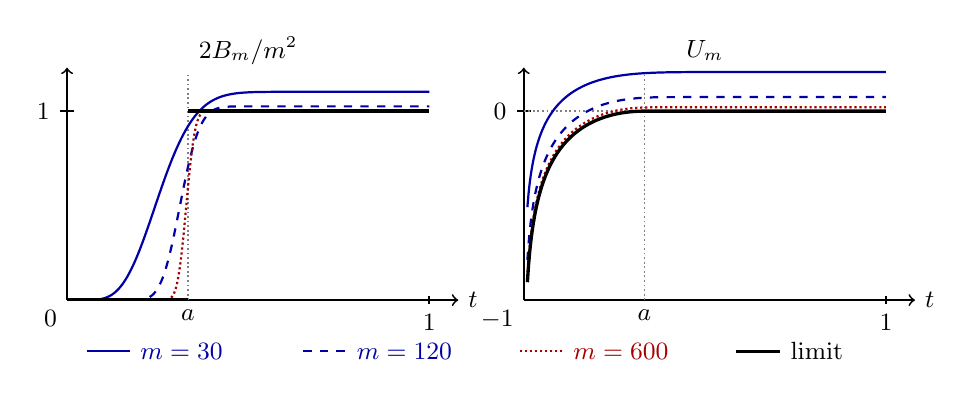
\begin{tikzpicture}[font=\small,line width=.65pt]
\begin{scope}[x=4.6cm,y=2.4cm]
\draw[->] (0,0)--(1.08,0) node[right] {$t$};
\draw[->] (0,0)--(0,1.23);
\node at (.5,1.32) {$2B_m/m^2$};
\node[below left] at (0,0) {$0$};
\draw (1,.02)--(1,-.02) node[below] {$1$};
\draw (.02,1)--(-.02,1) node[left] {$1$};
\draw[gray,densely dotted] (.333333,0)--(.333333,1.19);
\node[below] at (.333333,0) {$a$};
\begin{scope}\clip (0,0) rectangle (1,1.2);
\draw[blue!65!black,thick] plot coordinates {(0.000000,0.000000) (0.003333,0.000000) (0.006667,0.000000) (0.010000,0.000000) (0.013333,0.000000) (0.016667,0.000000) (0.020000,0.000000) (0.023333,0.000000) (0.026667,0.000001) (0.030000,0.000002) (0.033333,0.000005) (0.036667,0.000010) (0.040000,0.000019) (0.043333,0.000034) (0.046667,0.000057) (0.050000,0.000093) (0.053333,0.000146) (0.056667,0.000222) (0.060000,0.000328) (0.063333,0.000472) (0.066667,0.000665) (0.070000,0.000917) (0.073333,0.001243) (0.076667,0.001657) (0.080000,0.002175) (0.083333,0.002816) (0.086667,0.003598) (0.090000,0.004543) (0.093333,0.005672) (0.096667,0.007010) (0.100000,0.008579) (0.103333,0.010406) (0.106667,0.012516) (0.110000,0.014935) (0.113333,0.017689) (0.116667,0.020803) (0.120000,0.024304) (0.123333,0.028216) (0.126667,0.032564) (0.130000,0.037370) (0.133333,0.042656) (0.136667,0.048442) (0.140000,0.054746) (0.143333,0.061584) (0.146667,0.068971) (0.150000,0.076919) (0.153333,0.085436) (0.156667,0.094531) (0.160000,0.104207) (0.163333,0.114466) (0.166667,0.125308) (0.170000,0.136728) (0.173333,0.148721) (0.176667,0.161277) (0.180000,0.174384) (0.183333,0.188030) (0.186667,0.202196) (0.190000,0.216864) (0.193333,0.232014) (0.196667,0.247622) (0.200000,0.263662) (0.203333,0.280108) (0.206667,0.296932) (0.210000,0.314104) (0.213333,0.331593) (0.216667,0.349367) (0.220000,0.367393) (0.223333,0.385637) (0.226667,0.404066) (0.230000,0.422644) (0.233333,0.441339) (0.236667,0.460115) (0.240000,0.478939) (0.243333,0.497776) (0.246667,0.516594) (0.250000,0.535360) (0.253333,0.554044) (0.256667,0.572613) (0.260000,0.591040) (0.263333,0.609294) (0.266667,0.627351) (0.270000,0.645183) (0.273333,0.662766) (0.276667,0.680078) (0.280000,0.697098) (0.283333,0.713806) (0.286667,0.730183) (0.290000,0.746213) (0.293333,0.761882) (0.296667,0.777176) (0.300000,0.792083) (0.303333,0.806593) (0.306667,0.820698) (0.310000,0.834390) (0.313333,0.847664) (0.316667,0.860516) (0.320000,0.872943) (0.323333,0.884944) (0.326667,0.896518) (0.330000,0.907666) (0.333333,0.918390) (0.336667,0.928694) (0.340000,0.938582) (0.343333,0.948059) (0.346667,0.957130) (0.350000,0.965803) (0.353333,0.974084) (0.356667,0.981983) (0.360000,0.989507) (0.363333,0.996665) (0.366667,1.003469) (0.370000,1.009926) (0.373333,1.016048) (0.376667,1.021845) (0.380000,1.027329) (0.383333,1.032509) (0.386667,1.037397) (0.390000,1.042004) (0.393333,1.046341) (0.396667,1.050419) (0.400000,1.054249) (0.403333,1.057842) (0.406667,1.061209) (0.410000,1.064360) (0.413333,1.067306) (0.416667,1.070057) (0.420000,1.072622) (0.423333,1.075012) (0.426667,1.077236) (0.430000,1.079303) (0.433333,1.081221) (0.436667,1.083000) (0.440000,1.084648) (0.443333,1.086172) (0.446667,1.087580) (0.450000,1.088880) (0.453333,1.090078) (0.456667,1.091181) (0.460000,1.092195) (0.463333,1.093126) (0.466667,1.093981) (0.470000,1.094764) (0.473333,1.095480) (0.476667,1.096135) (0.480000,1.096733) (0.483333,1.097278) (0.486667,1.097774) (0.490000,1.098225) (0.493333,1.098635) (0.496667,1.099007) (0.500000,1.099344) (0.503333,1.099649) (0.506667,1.099924) (0.510000,1.100173) (0.513333,1.100397) (0.516667,1.100599) (0.520000,1.100780) (0.523333,1.100943) (0.526667,1.101089) (0.530000,1.101219) (0.533333,1.101336) (0.536667,1.101441) (0.540000,1.101534) (0.543333,1.101616) (0.546667,1.101690) (0.550000,1.101755) (0.553333,1.101813) (0.556667,1.101864) (0.560000,1.101910) (0.563333,1.101950) (0.566667,1.101985) (0.570000,1.102016) (0.573333,1.102043) (0.576667,1.102067) (0.580000,1.102088) (0.583333,1.102106) (0.586667,1.102122) (0.590000,1.102136) (0.593333,1.102148) (0.596667,1.102159) (0.600000,1.102168) (0.603333,1.102176) (0.606667,1.102183) (0.610000,1.102188) (0.613333,1.102193) (0.616667,1.102198) (0.620000,1.102202) (0.623333,1.102205) (0.626667,1.102207) (0.630000,1.102210) (0.633333,1.102212) (0.636667,1.102213) (0.640000,1.102215) (0.643333,1.102216) (0.646667,1.102217) (0.650000,1.102218) (0.653333,1.102219) (0.656667,1.102219) (0.660000,1.102220) (0.663333,1.102220) (0.666667,1.102221) (0.670000,1.102221) (0.673333,1.102221) (0.676667,1.102221) (0.680000,1.102221) (0.683333,1.102222) (0.686667,1.102222) (0.690000,1.102222) (0.693333,1.102222) (0.696667,1.102222) (0.700000,1.102222) (0.703333,1.102222) (0.706667,1.102222) (0.710000,1.102222) (0.713333,1.102222) (0.716667,1.102222) (0.720000,1.102222) (0.723333,1.102222) (0.726667,1.102222) (0.730000,1.102222) (0.733333,1.102222) (0.736667,1.102222) (0.740000,1.102222) (0.743333,1.102222) (0.746667,1.102222) (0.750000,1.102222) (0.753333,1.102222) (0.756667,1.102222) (0.760000,1.102222) (0.763333,1.102222) (0.766667,1.102222) (0.770000,1.102222) (0.773333,1.102222) (0.776667,1.102222) (0.780000,1.102222) (0.783333,1.102222) (0.786667,1.102222) (0.790000,1.102222) (0.793333,1.102222) (0.796667,1.102222) (0.800000,1.102222) (0.803333,1.102222) (0.806667,1.102222) (0.810000,1.102222) (0.813333,1.102222) (0.816667,1.102222) (0.820000,1.102222) (0.823333,1.102222) (0.826667,1.102222) (0.830000,1.102222) (0.833333,1.102222) (0.836667,1.102222) (0.840000,1.102222) (0.843333,1.102222) (0.846667,1.102222) (0.850000,1.102222) (0.853333,1.102222) (0.856667,1.102222) (0.860000,1.102222) (0.863333,1.102222) (0.866667,1.102222) (0.870000,1.102222) (0.873333,1.102222) (0.876667,1.102222) (0.880000,1.102222) (0.883333,1.102222) (0.886667,1.102222) (0.890000,1.102222) (0.893333,1.102222) (0.896667,1.102222) (0.900000,1.102222) (0.903333,1.102222) (0.906667,1.102222) (0.910000,1.102222) (0.913333,1.102222) (0.916667,1.102222) (0.920000,1.102222) (0.923333,1.102222) (0.926667,1.102222) (0.930000,1.102222) (0.933333,1.102222) (0.936667,1.102222) (0.940000,1.102222) (0.943333,1.102222) (0.946667,1.102222) (0.950000,1.102222) (0.953333,1.102222) (0.956667,1.102222) (0.960000,1.102222) (0.963333,1.102222) (0.966667,1.102222) (0.970000,1.102222) (0.973333,1.102222) (0.976667,1.102222) (0.980000,1.102222) (0.983333,1.102222) (0.986667,1.102222) (0.990000,1.102222) (0.993333,1.102222) (0.996667,1.102222) (1.000000,1.102222)};
\draw[blue!65!black,dashed,thick] plot coordinates {(0.000000,0.000000) (0.003333,0.000000) (0.006667,0.000000) (0.010000,0.000000) (0.013333,0.000000) (0.016667,0.000000) (0.020000,0.000000) (0.023333,0.000000) (0.026667,0.000000) (0.030000,0.000000) (0.033333,0.000000) (0.036667,0.000000) (0.040000,0.000000) (0.043333,0.000000) (0.046667,0.000000) (0.050000,0.000000) (0.053333,0.000000) (0.056667,0.000000) (0.060000,0.000000) (0.063333,0.000000) (0.066667,0.000000) (0.070000,0.000000) (0.073333,0.000000) (0.076667,0.000000) (0.080000,0.000000) (0.083333,0.000000) (0.086667,0.000000) (0.090000,0.000000) (0.093333,0.000000) (0.096667,0.000000) (0.100000,0.000000) (0.103333,0.000000) (0.106667,0.000000) (0.110000,0.000000) (0.113333,0.000000) (0.116667,0.000000) (0.120000,0.000000) (0.123333,0.000000) (0.126667,0.000000) (0.130000,0.000000) (0.133333,0.000000) (0.136667,0.000000) (0.140000,0.000001) (0.143333,0.000001) (0.146667,0.000002) (0.150000,0.000003) (0.153333,0.000006) (0.156667,0.000010) (0.160000,0.000016) (0.163333,0.000026) (0.166667,0.000041) (0.170000,0.000063) (0.173333,0.000096) (0.176667,0.000145) (0.180000,0.000215) (0.183333,0.000315) (0.186667,0.000454) (0.190000,0.000648) (0.193333,0.000912) (0.196667,0.001267) (0.200000,0.001741) (0.203333,0.002365) (0.206667,0.003176) (0.210000,0.004220) (0.213333,0.005549) (0.216667,0.007222) (0.220000,0.009308) (0.223333,0.011880) (0.226667,0.015023) (0.230000,0.018825) (0.233333,0.023383) (0.236667,0.028795) (0.240000,0.035165) (0.243333,0.042597) (0.246667,0.051193) (0.250000,0.061052) (0.253333,0.072266) (0.256667,0.084919) (0.260000,0.099083) (0.263333,0.114813) (0.266667,0.132150) (0.270000,0.151114) (0.273333,0.171706) (0.276667,0.193902) (0.280000,0.217657) (0.283333,0.242902) (0.286667,0.269544) (0.290000,0.297469) (0.293333,0.326543) (0.296667,0.356611) (0.300000,0.387506) (0.303333,0.419044) (0.306667,0.451035) (0.310000,0.483282) (0.313333,0.515583) (0.316667,0.547742) (0.320000,0.579564) (0.323333,0.610865) (0.326667,0.641470) (0.330000,0.671219) (0.333333,0.699967) (0.336667,0.727589) (0.340000,0.753977) (0.343333,0.779044) (0.346667,0.802722) (0.350000,0.824965) (0.353333,0.845743) (0.356667,0.865046) (0.360000,0.882883) (0.363333,0.899276) (0.366667,0.914260) (0.370000,0.927884) (0.373333,0.940205) (0.376667,0.951290) (0.380000,0.961210) (0.383333,0.970041) (0.386667,0.977863) (0.390000,0.984754) (0.393333,0.990794) (0.396667,0.996061) (0.400000,1.000631) (0.403333,1.004575) (0.406667,1.007963) (0.410000,1.010857) (0.413333,1.013317) (0.416667,1.015398) (0.420000,1.017150) (0.423333,1.018616) (0.426667,1.019838) (0.430000,1.020851) (0.433333,1.021686) (0.436667,1.022372) (0.440000,1.022931) (0.443333,1.023386) (0.446667,1.023754) (0.450000,1.024049) (0.453333,1.024286) (0.456667,1.024474) (0.460000,1.024624) (0.463333,1.024741) (0.466667,1.024833) (0.470000,1.024905) (0.473333,1.024961) (0.476667,1.025005) (0.480000,1.025038) (0.483333,1.025063) (0.486667,1.025082) (0.490000,1.025097) (0.493333,1.025108) (0.496667,1.025116) (0.500000,1.025122) (0.503333,1.025127) (0.506667,1.025130) (0.510000,1.025133) (0.513333,1.025134) (0.516667,1.025136) (0.520000,1.025137) (0.523333,1.025137) (0.526667,1.025138) (0.530000,1.025138) (0.533333,1.025138) (0.536667,1.025139) (0.540000,1.025139) (0.543333,1.025139) (0.546667,1.025139) (0.550000,1.025139) (0.553333,1.025139) (0.556667,1.025139) (0.560000,1.025139) (0.563333,1.025139) (0.566667,1.025139) (0.570000,1.025139) (0.573333,1.025139) (0.576667,1.025139) (0.580000,1.025139) (0.583333,1.025139) (0.586667,1.025139) (0.590000,1.025139) (0.593333,1.025139) (0.596667,1.025139) (0.600000,1.025139) (0.603333,1.025139) (0.606667,1.025139) (0.610000,1.025139) (0.613333,1.025139) (0.616667,1.025139) (0.620000,1.025139) (0.623333,1.025139) (0.626667,1.025139) (0.630000,1.025139) (0.633333,1.025139) (0.636667,1.025139) (0.640000,1.025139) (0.643333,1.025139) (0.646667,1.025139) (0.650000,1.025139) (0.653333,1.025139) (0.656667,1.025139) (0.660000,1.025139) (0.663333,1.025139) (0.666667,1.025139) (0.670000,1.025139) (0.673333,1.025139) (0.676667,1.025139) (0.680000,1.025139) (0.683333,1.025139) (0.686667,1.025139) (0.690000,1.025139) (0.693333,1.025139) (0.696667,1.025139) (0.700000,1.025139) (0.703333,1.025139) (0.706667,1.025139) (0.710000,1.025139) (0.713333,1.025139) (0.716667,1.025139) (0.720000,1.025139) (0.723333,1.025139) (0.726667,1.025139) (0.730000,1.025139) (0.733333,1.025139) (0.736667,1.025139) (0.740000,1.025139) (0.743333,1.025139) (0.746667,1.025139) (0.750000,1.025139) (0.753333,1.025139) (0.756667,1.025139) (0.760000,1.025139) (0.763333,1.025139) (0.766667,1.025139) (0.770000,1.025139) (0.773333,1.025139) (0.776667,1.025139) (0.780000,1.025139) (0.783333,1.025139) (0.786667,1.025139) (0.790000,1.025139) (0.793333,1.025139) (0.796667,1.025139) (0.800000,1.025139) (0.803333,1.025139) (0.806667,1.025139) (0.810000,1.025139) (0.813333,1.025139) (0.816667,1.025139) (0.820000,1.025139) (0.823333,1.025139) (0.826667,1.025139) (0.830000,1.025139) (0.833333,1.025139) (0.836667,1.025139) (0.840000,1.025139) (0.843333,1.025139) (0.846667,1.025139) (0.850000,1.025139) (0.853333,1.025139) (0.856667,1.025139) (0.860000,1.025139) (0.863333,1.025139) (0.866667,1.025139) (0.870000,1.025139) (0.873333,1.025139) (0.876667,1.025139) (0.880000,1.025139) (0.883333,1.025139) (0.886667,1.025139) (0.890000,1.025139) (0.893333,1.025139) (0.896667,1.025139) (0.900000,1.025139) (0.903333,1.025139) (0.906667,1.025139) (0.910000,1.025139) (0.913333,1.025139) (0.916667,1.025139) (0.920000,1.025139) (0.923333,1.025139) (0.926667,1.025139) (0.930000,1.025139) (0.933333,1.025139) (0.936667,1.025139) (0.940000,1.025139) (0.943333,1.025139) (0.946667,1.025139) (0.950000,1.025139) (0.953333,1.025139) (0.956667,1.025139) (0.960000,1.025139) (0.963333,1.025139) (0.966667,1.025139) (0.970000,1.025139) (0.973333,1.025139) (0.976667,1.025139) (0.980000,1.025139) (0.983333,1.025139) (0.986667,1.025139) (0.990000,1.025139) (0.993333,1.025139) (0.996667,1.025139) (1.000000,1.025139)};
\draw[red!65!black,densely dotted,thick] plot coordinates {(0.000000,0.000000) (0.003333,0.000000) (0.006667,0.000000) (0.010000,0.000000) (0.013333,0.000000) (0.016667,0.000000) (0.020000,0.000000) (0.023333,0.000000) (0.026667,0.000000) (0.030000,0.000000) (0.033333,0.000000) (0.036667,0.000000) (0.040000,0.000000) (0.043333,0.000000) (0.046667,0.000000) (0.050000,0.000000) (0.053333,0.000000) (0.056667,0.000000) (0.060000,0.000000) (0.063333,0.000000) (0.066667,0.000000) (0.070000,0.000000) (0.073333,0.000000) (0.076667,0.000000) (0.080000,0.000000) (0.083333,0.000000) (0.086667,0.000000) (0.090000,0.000000) (0.093333,0.000000) (0.096667,0.000000) (0.100000,0.000000) (0.103333,0.000000) (0.106667,0.000000) (0.110000,0.000000) (0.113333,0.000000) (0.116667,0.000000) (0.120000,0.000000) (0.123333,0.000000) (0.126667,0.000000) (0.130000,0.000000) (0.133333,0.000000) (0.136667,0.000000) (0.140000,0.000000) (0.143333,0.000000) (0.146667,0.000000) (0.150000,0.000000) (0.153333,0.000000) (0.156667,0.000000) (0.160000,0.000000) (0.163333,0.000000) (0.166667,0.000000) (0.170000,0.000000) (0.173333,0.000000) (0.176667,0.000000) (0.180000,0.000000) (0.183333,0.000000) (0.186667,0.000000) (0.190000,0.000000) (0.193333,0.000000) (0.196667,0.000000) (0.200000,0.000000) (0.203333,0.000000) (0.206667,0.000000) (0.210000,0.000000) (0.213333,0.000000) (0.216667,0.000000) (0.220000,0.000000) (0.223333,0.000000) (0.226667,0.000000) (0.230000,0.000000) (0.233333,0.000000) (0.236667,0.000000) (0.240000,0.000000) (0.243333,0.000001) (0.246667,0.000003) (0.250000,0.000007) (0.253333,0.000016) (0.256667,0.000037) (0.260000,0.000081) (0.263333,0.000171) (0.266667,0.000348) (0.270000,0.000681) (0.273333,0.001284) (0.276667,0.002337) (0.280000,0.004106) (0.283333,0.006973) (0.286667,0.011454) (0.290000,0.018212) (0.293333,0.028056) (0.296667,0.041907) (0.300000,0.060743) (0.303333,0.085513) (0.306667,0.117026) (0.310000,0.155828) (0.313333,0.202089) (0.316667,0.255512) (0.320000,0.315292) (0.323333,0.380137) (0.326667,0.448342) (0.330000,0.517931) (0.333333,0.586824) (0.336667,0.653023) (0.340000,0.714784) (0.343333,0.770742) (0.346667,0.819993) (0.350000,0.862114) (0.353333,0.897125) (0.356667,0.925415) (0.360000,0.947641) (0.363333,0.964625) (0.366667,0.977249) (0.370000,0.986378) (0.373333,0.992802) (0.376667,0.997202) (0.380000,1.000136) (0.383333,1.002039) (0.386667,1.003243) (0.390000,1.003983) (0.393333,1.004427) (0.396667,1.004686) (0.400000,1.004833) (0.403333,1.004915) (0.406667,1.004959) (0.410000,1.004982) (0.413333,1.004994) (0.416667,1.005000) (0.420000,1.005003) (0.423333,1.005004) (0.426667,1.005005) (0.430000,1.005005) (0.433333,1.005005) (0.436667,1.005006) (0.440000,1.005006) (0.443333,1.005006) (0.446667,1.005006) (0.450000,1.005006) (0.453333,1.005006) (0.456667,1.005006) (0.460000,1.005006) (0.463333,1.005006) (0.466667,1.005006) (0.470000,1.005006) (0.473333,1.005006) (0.476667,1.005006) (0.480000,1.005006) (0.483333,1.005006) (0.486667,1.005006) (0.490000,1.005006) (0.493333,1.005006) (0.496667,1.005006) (0.500000,1.005006) (0.503333,1.005006) (0.506667,1.005006) (0.510000,1.005006) (0.513333,1.005006) (0.516667,1.005006) (0.520000,1.005006) (0.523333,1.005006) (0.526667,1.005006) (0.530000,1.005006) (0.533333,1.005006) (0.536667,1.005006) (0.540000,1.005006) (0.543333,1.005006) (0.546667,1.005006) (0.550000,1.005006) (0.553333,1.005006) (0.556667,1.005006) (0.560000,1.005006) (0.563333,1.005006) (0.566667,1.005006) (0.570000,1.005006) (0.573333,1.005006) (0.576667,1.005006) (0.580000,1.005006) (0.583333,1.005006) (0.586667,1.005006) (0.590000,1.005006) (0.593333,1.005006) (0.596667,1.005006) (0.600000,1.005006) (0.603333,1.005006) (0.606667,1.005006) (0.610000,1.005006) (0.613333,1.005006) (0.616667,1.005006) (0.620000,1.005006) (0.623333,1.005006) (0.626667,1.005006) (0.630000,1.005006) (0.633333,1.005006) (0.636667,1.005006) (0.640000,1.005006) (0.643333,1.005006) (0.646667,1.005006) (0.650000,1.005006) (0.653333,1.005006) (0.656667,1.005006) (0.660000,1.005006) (0.663333,1.005006) (0.666667,1.005006) (0.670000,1.005006) (0.673333,1.005006) (0.676667,1.005006) (0.680000,1.005006) (0.683333,1.005006) (0.686667,1.005006) (0.690000,1.005006) (0.693333,1.005006) (0.696667,1.005006) (0.700000,1.005006) (0.703333,1.005006) (0.706667,1.005006) (0.710000,1.005006) (0.713333,1.005006) (0.716667,1.005006) (0.720000,1.005006) (0.723333,1.005006) (0.726667,1.005006) (0.730000,1.005006) (0.733333,1.005006) (0.736667,1.005006) (0.740000,1.005006) (0.743333,1.005006) (0.746667,1.005006) (0.750000,1.005006) (0.753333,1.005006) (0.756667,1.005006) (0.760000,1.005006) (0.763333,1.005006) (0.766667,1.005006) (0.770000,1.005006) (0.773333,1.005006) (0.776667,1.005006) (0.780000,1.005006) (0.783333,1.005006) (0.786667,1.005006) (0.790000,1.005006) (0.793333,1.005006) (0.796667,1.005006) (0.800000,1.005006) (0.803333,1.005006) (0.806667,1.005006) (0.810000,1.005006) (0.813333,1.005006) (0.816667,1.005006) (0.820000,1.005006) (0.823333,1.005006) (0.826667,1.005006) (0.830000,1.005006) (0.833333,1.005006) (0.836667,1.005006) (0.840000,1.005006) (0.843333,1.005006) (0.846667,1.005006) (0.850000,1.005006) (0.853333,1.005006) (0.856667,1.005006) (0.860000,1.005006) (0.863333,1.005006) (0.866667,1.005006) (0.870000,1.005006) (0.873333,1.005006) (0.876667,1.005006) (0.880000,1.005006) (0.883333,1.005006) (0.886667,1.005006) (0.890000,1.005006) (0.893333,1.005006) (0.896667,1.005006) (0.900000,1.005006) (0.903333,1.005006) (0.906667,1.005006) (0.910000,1.005006) (0.913333,1.005006) (0.916667,1.005006) (0.920000,1.005006) (0.923333,1.005006) (0.926667,1.005006) (0.930000,1.005006) (0.933333,1.005006) (0.936667,1.005006) (0.940000,1.005006) (0.943333,1.005006) (0.946667,1.005006) (0.950000,1.005006) (0.953333,1.005006) (0.956667,1.005006) (0.960000,1.005006) (0.963333,1.005006) (0.966667,1.005006) (0.970000,1.005006) (0.973333,1.005006) (0.976667,1.005006) (0.980000,1.005006) (0.983333,1.005006) (0.986667,1.005006) (0.990000,1.005006) (0.993333,1.005006) (0.996667,1.005006) (1.000000,1.005006)};
\draw[black,very thick] (0,0)--(.333333,0);
\draw[black,very thick] (.333333,1)--(1,1);
\end{scope}\end{scope}
\begin{scope}[xshift=5.8cm,x=4.6cm,y=2.4cm]
\draw[->] (0,0)--(1.08,0) node[right] {$t$};
\draw[->] (0,0)--(0,1.23);
\node at (.5,1.32) {$U_m$};
\node[below left] at (0,0) {$-1$};
\draw (1,.02)--(1,-.02) node[below] {$1$};
\draw (.02,1)--(-.02,1) node[left] {$0$};
\draw[gray,densely dotted] (0,1)--(1,1);
\draw[gray,densely dotted] (.333333,0)--(.333333,1.19);
\node[below] at (.333333,0) {$a$};
\begin{scope}\clip (0,0) rectangle (1,1.22);
\draw[blue!65!black,thick] plot coordinates {(0.010000,0.491716) (0.013300,0.565596) (0.016600,0.622527) (0.019900,0.668702) (0.023200,0.707436) (0.026500,0.740715) (0.029800,0.769821) (0.033100,0.795633) (0.036400,0.818776) (0.039700,0.839714) (0.043000,0.858799) (0.046300,0.876304) (0.049600,0.892446) (0.052900,0.907401) (0.056200,0.921311) (0.059500,0.934297) (0.062800,0.946456) (0.066100,0.957874) (0.069400,0.968621) (0.072700,0.978761) (0.076000,0.988347) (0.079300,0.997426) (0.082600,1.006038) (0.085900,1.014219) (0.089200,1.022003) (0.092500,1.029418) (0.095800,1.036489) (0.099100,1.043240) (0.102400,1.049691) (0.105700,1.055861) (0.109000,1.061767) (0.112300,1.067424) (0.115600,1.072848) (0.118900,1.078051) (0.122200,1.083045) (0.125500,1.087840) (0.128800,1.092448) (0.132100,1.096877) (0.135400,1.101137) (0.138700,1.105235) (0.142000,1.109178) (0.145300,1.112975) (0.148600,1.116631) (0.151900,1.120153) (0.155200,1.123546) (0.158500,1.126816) (0.161800,1.129967) (0.165100,1.133005) (0.168400,1.135934) (0.171700,1.138758) (0.175000,1.141482) (0.178300,1.144109) (0.181600,1.146642) (0.184900,1.149085) (0.188200,1.151442) (0.191500,1.153715) (0.194800,1.155908) (0.198100,1.158022) (0.201400,1.160061) (0.204700,1.162028) (0.208000,1.163924) (0.211300,1.165753) (0.214600,1.167516) (0.217900,1.169215) (0.221200,1.170853) (0.224500,1.172431) (0.227800,1.173951) (0.231100,1.175416) (0.234400,1.176827) (0.237700,1.178185) (0.241000,1.179493) (0.244300,1.180752) (0.247600,1.181963) (0.250900,1.183128) (0.254200,1.184248) (0.257500,1.185325) (0.260800,1.186360) (0.264100,1.187354) (0.267400,1.188309) (0.270700,1.189226) (0.274000,1.190105) (0.277300,1.190949) (0.280600,1.191759) (0.283900,1.192534) (0.287200,1.193278) (0.290500,1.193989) (0.293800,1.194671) (0.297100,1.195323) (0.300400,1.195946) (0.303700,1.196542) (0.307000,1.197111) (0.310300,1.197655) (0.313600,1.198174) (0.316900,1.198668) (0.320200,1.199140) (0.323500,1.199589) (0.326800,1.200017) (0.330100,1.200424) (0.333400,1.200811) (0.336700,1.201179) (0.340000,1.201529) (0.343300,1.201860) (0.346600,1.202175) (0.349900,1.202473) (0.353200,1.202755) (0.356500,1.203022) (0.359800,1.203275) (0.363100,1.203514) (0.366400,1.203739) (0.369700,1.203952) (0.373000,1.204153) (0.376300,1.204342) (0.379600,1.204519) (0.382900,1.204687) (0.386200,1.204844) (0.389500,1.204992) (0.392800,1.205130) (0.396100,1.205260) (0.399400,1.205381) (0.402700,1.205495) (0.406000,1.205601) (0.409300,1.205701) (0.412600,1.205793) (0.415900,1.205879) (0.419200,1.205960) (0.422500,1.206035) (0.425800,1.206104) (0.429100,1.206169) (0.432400,1.206229) (0.435700,1.206284) (0.439000,1.206335) (0.442300,1.206383) (0.445600,1.206427) (0.448900,1.206467) (0.452200,1.206504) (0.455500,1.206539) (0.458800,1.206570) (0.462100,1.206599) (0.465400,1.206626) (0.468700,1.206650) (0.472000,1.206673) (0.475300,1.206693) (0.478600,1.206712) (0.481900,1.206729) (0.485200,1.206745) (0.488500,1.206759) (0.491800,1.206772) (0.495100,1.206783) (0.498400,1.206794) (0.501700,1.206804) (0.505000,1.206812) (0.508300,1.206820) (0.511600,1.206827) (0.514900,1.206834) (0.518200,1.206839) (0.521500,1.206845) (0.524800,1.206849) (0.528100,1.206853) (0.531400,1.206857) (0.534700,1.206860) (0.538000,1.206863) (0.541300,1.206866) (0.544600,1.206868) (0.547900,1.206871) (0.551200,1.206872) (0.554500,1.206874) (0.557800,1.206876) (0.561100,1.206877) (0.564400,1.206878) (0.567700,1.206879) (0.571000,1.206880) (0.574300,1.206881) (0.577600,1.206881) (0.580900,1.206882) (0.584200,1.206882) (0.587500,1.206883) (0.590800,1.206883) (0.594100,1.206884) (0.597400,1.206884) (0.600700,1.206884) (0.604000,1.206885) (0.607300,1.206885) (0.610600,1.206885) (0.613900,1.206885) (0.617200,1.206885) (0.620500,1.206885) (0.623800,1.206885) (0.627100,1.206885) (0.630400,1.206885) (0.633700,1.206886) (0.637000,1.206886) (0.640300,1.206886) (0.643600,1.206886) (0.646900,1.206886) (0.650200,1.206886) (0.653500,1.206886) (0.656800,1.206886) (0.660100,1.206886) (0.663400,1.206886) (0.666700,1.206886) (0.670000,1.206886) (0.673300,1.206886) (0.676600,1.206886) (0.679900,1.206886) (0.683200,1.206886) (0.686500,1.206886) (0.689800,1.206886) (0.693100,1.206886) (0.696400,1.206886) (0.699700,1.206886) (0.703000,1.206886) (0.706300,1.206886) (0.709600,1.206886) (0.712900,1.206886) (0.716200,1.206886) (0.719500,1.206886) (0.722800,1.206886) (0.726100,1.206886) (0.729400,1.206886) (0.732700,1.206886) (0.736000,1.206886) (0.739300,1.206886) (0.742600,1.206886) (0.745900,1.206886) (0.749200,1.206886) (0.752500,1.206886) (0.755800,1.206886) (0.759100,1.206886) (0.762400,1.206886) (0.765700,1.206886) (0.769000,1.206886) (0.772300,1.206886) (0.775600,1.206886) (0.778900,1.206886) (0.782200,1.206886) (0.785500,1.206886) (0.788800,1.206886) (0.792100,1.206886) (0.795400,1.206886) (0.798700,1.206886) (0.802000,1.206886) (0.805300,1.206886) (0.808600,1.206886) (0.811900,1.206886) (0.815200,1.206886) (0.818500,1.206886) (0.821800,1.206886) (0.825100,1.206886) (0.828400,1.206886) (0.831700,1.206886) (0.835000,1.206886) (0.838300,1.206886) (0.841600,1.206886) (0.844900,1.206886) (0.848200,1.206886) (0.851500,1.206886) (0.854800,1.206886) (0.858100,1.206886) (0.861400,1.206886) (0.864700,1.206886) (0.868000,1.206886) (0.871300,1.206886) (0.874600,1.206886) (0.877900,1.206886) (0.881200,1.206886) (0.884500,1.206886) (0.887800,1.206886) (0.891100,1.206886) (0.894400,1.206886) (0.897700,1.206886) (0.901000,1.206886) (0.904300,1.206886) (0.907600,1.206886) (0.910900,1.206886) (0.914200,1.206886) (0.917500,1.206886) (0.920800,1.206886) (0.924100,1.206886) (0.927400,1.206886) (0.930700,1.206886) (0.934000,1.206886) (0.937300,1.206886) (0.940600,1.206886) (0.943900,1.206886) (0.947200,1.206886) (0.950500,1.206886) (0.953800,1.206886) (0.957100,1.206886) (0.960400,1.206886) (0.963700,1.206886) (0.967000,1.206886) (0.970300,1.206886) (0.973600,1.206886) (0.976900,1.206886) (0.980200,1.206886) (0.983500,1.206886) (0.986800,1.206886) (0.990100,1.206886) (0.993400,1.206886) (0.996700,1.206886) (1.000000,1.206886)};
\draw[blue!65!black,dashed,thick] plot coordinates {(0.010000,0.212312) (0.013300,0.300397) (0.016600,0.368355) (0.019900,0.423538) (0.023200,0.469883) (0.026500,0.509749) (0.029800,0.544658) (0.033100,0.575654) (0.036400,0.603479) (0.039700,0.628684) (0.043000,0.651685) (0.046300,0.672810) (0.049600,0.692314) (0.052900,0.710406) (0.056200,0.727256) (0.059500,0.743006) (0.062800,0.757772) (0.066100,0.771655) (0.069400,0.784741) (0.072700,0.797103) (0.076000,0.808804) (0.079300,0.819900) (0.082600,0.830440) (0.085900,0.840466) (0.089200,0.850017) (0.092500,0.859127) (0.095800,0.867826) (0.099100,0.876142) (0.102400,0.884098) (0.105700,0.891718) (0.109000,0.899021) (0.112300,0.906026) (0.115600,0.912750) (0.118900,0.919208) (0.122200,0.925414) (0.125500,0.931381) (0.128800,0.937122) (0.132100,0.942646) (0.135400,0.947965) (0.138700,0.953088) (0.142000,0.958024) (0.145300,0.962781) (0.148600,0.967366) (0.151900,0.971788) (0.155200,0.976052) (0.158500,0.980165) (0.161800,0.984133) (0.165100,0.987961) (0.168400,0.991654) (0.171700,0.995218) (0.175000,0.998657) (0.178300,1.001976) (0.181600,1.005178) (0.184900,1.008268) (0.188200,1.011249) (0.191500,1.014125) (0.194800,1.016899) (0.198100,1.019575) (0.201400,1.022155) (0.204700,1.024642) (0.208000,1.027040) (0.211300,1.029350) (0.214600,1.031576) (0.217900,1.033719) (0.221200,1.035782) (0.224500,1.037768) (0.227800,1.039678) (0.231100,1.041515) (0.234400,1.043280) (0.237700,1.044976) (0.241000,1.046604) (0.244300,1.048166) (0.247600,1.049665) (0.250900,1.051101) (0.254200,1.052476) (0.257500,1.053792) (0.260800,1.055050) (0.264100,1.056253) (0.267400,1.057401) (0.270700,1.058496) (0.274000,1.059539) (0.277300,1.060532) (0.280600,1.061477) (0.283900,1.062374) (0.287200,1.063225) (0.290500,1.064031) (0.293800,1.064794) (0.297100,1.065515) (0.300400,1.066195) (0.303700,1.066836) (0.307000,1.067439) (0.310300,1.068006) (0.313600,1.068536) (0.316900,1.069033) (0.320200,1.069497) (0.323500,1.069929) (0.326800,1.070331) (0.330100,1.070704) (0.333400,1.071049) (0.336700,1.071368) (0.340000,1.071662) (0.343300,1.071932) (0.346600,1.072179) (0.349900,1.072405) (0.353200,1.072611) (0.356500,1.072798) (0.359800,1.072968) (0.363100,1.073120) (0.366400,1.073258) (0.369700,1.073381) (0.373000,1.073491) (0.376300,1.073589) (0.379600,1.073676) (0.382900,1.073752) (0.386200,1.073820) (0.389500,1.073879) (0.392800,1.073931) (0.396100,1.073975) (0.399400,1.074014) (0.402700,1.074047) (0.406000,1.074076) (0.409300,1.074101) (0.412600,1.074121) (0.415900,1.074139) (0.419200,1.074154) (0.422500,1.074166) (0.425800,1.074177) (0.429100,1.074185) (0.432400,1.074192) (0.435700,1.074198) (0.439000,1.074203) (0.442300,1.074207) (0.445600,1.074210) (0.448900,1.074213) (0.452200,1.074215) (0.455500,1.074216) (0.458800,1.074218) (0.462100,1.074219) (0.465400,1.074219) (0.468700,1.074220) (0.472000,1.074221) (0.475300,1.074221) (0.478600,1.074221) (0.481900,1.074222) (0.485200,1.074222) (0.488500,1.074222) (0.491800,1.074222) (0.495100,1.074222) (0.498400,1.074222) (0.501700,1.074222) (0.505000,1.074222) (0.508300,1.074222) (0.511600,1.074222) (0.514900,1.074222) (0.518200,1.074222) (0.521500,1.074222) (0.524800,1.074222) (0.528100,1.074222) (0.531400,1.074222) (0.534700,1.074222) (0.538000,1.074222) (0.541300,1.074222) (0.544600,1.074222) (0.547900,1.074222) (0.551200,1.074222) (0.554500,1.074222) (0.557800,1.074222) (0.561100,1.074222) (0.564400,1.074222) (0.567700,1.074222) (0.571000,1.074222) (0.574300,1.074222) (0.577600,1.074222) (0.580900,1.074222) (0.584200,1.074222) (0.587500,1.074222) (0.590800,1.074222) (0.594100,1.074222) (0.597400,1.074222) (0.600700,1.074222) (0.604000,1.074222) (0.607300,1.074222) (0.610600,1.074222) (0.613900,1.074222) (0.617200,1.074222) (0.620500,1.074222) (0.623800,1.074222) (0.627100,1.074222) (0.630400,1.074222) (0.633700,1.074222) (0.637000,1.074222) (0.640300,1.074222) (0.643600,1.074222) (0.646900,1.074222) (0.650200,1.074222) (0.653500,1.074222) (0.656800,1.074222) (0.660100,1.074222) (0.663400,1.074222) (0.666700,1.074222) (0.670000,1.074222) (0.673300,1.074222) (0.676600,1.074222) (0.679900,1.074222) (0.683200,1.074222) (0.686500,1.074222) (0.689800,1.074222) (0.693100,1.074222) (0.696400,1.074222) (0.699700,1.074222) (0.703000,1.074222) (0.706300,1.074222) (0.709600,1.074222) (0.712900,1.074222) (0.716200,1.074222) (0.719500,1.074222) (0.722800,1.074222) (0.726100,1.074222) (0.729400,1.074222) (0.732700,1.074222) (0.736000,1.074222) (0.739300,1.074222) (0.742600,1.074222) (0.745900,1.074222) (0.749200,1.074222) (0.752500,1.074222) (0.755800,1.074222) (0.759100,1.074222) (0.762400,1.074222) (0.765700,1.074222) (0.769000,1.074222) (0.772300,1.074222) (0.775600,1.074222) (0.778900,1.074222) (0.782200,1.074222) (0.785500,1.074222) (0.788800,1.074222) (0.792100,1.074222) (0.795400,1.074222) (0.798700,1.074222) (0.802000,1.074222) (0.805300,1.074222) (0.808600,1.074222) (0.811900,1.074222) (0.815200,1.074222) (0.818500,1.074222) (0.821800,1.074222) (0.825100,1.074222) (0.828400,1.074222) (0.831700,1.074222) (0.835000,1.074222) (0.838300,1.074222) (0.841600,1.074222) (0.844900,1.074222) (0.848200,1.074222) (0.851500,1.074222) (0.854800,1.074222) (0.858100,1.074222) (0.861400,1.074222) (0.864700,1.074222) (0.868000,1.074222) (0.871300,1.074222) (0.874600,1.074222) (0.877900,1.074222) (0.881200,1.074222) (0.884500,1.074222) (0.887800,1.074222) (0.891100,1.074222) (0.894400,1.074222) (0.897700,1.074222) (0.901000,1.074222) (0.904300,1.074222) (0.907600,1.074222) (0.910900,1.074222) (0.914200,1.074222) (0.917500,1.074222) (0.920800,1.074222) (0.924100,1.074222) (0.927400,1.074222) (0.930700,1.074222) (0.934000,1.074222) (0.937300,1.074222) (0.940600,1.074222) (0.943900,1.074222) (0.947200,1.074222) (0.950500,1.074222) (0.953800,1.074222) (0.957100,1.074222) (0.960400,1.074222) (0.963700,1.074222) (0.967000,1.074222) (0.970300,1.074222) (0.973600,1.074222) (0.976900,1.074222) (0.980200,1.074222) (0.983500,1.074222) (0.986800,1.074222) (0.990100,1.074222) (0.993400,1.074222) (0.996700,1.074222) (1.000000,1.074222)};
\draw[red!65!black,densely dotted,thick] plot coordinates {(0.010000,0.122344) (0.013300,0.214227) (0.016600,0.285135) (0.019900,0.342730) (0.023200,0.391115) (0.026500,0.432748) (0.029800,0.469215) (0.033100,0.501603) (0.036400,0.530687) (0.039700,0.557040) (0.043000,0.581097) (0.046300,0.603197) (0.049600,0.623608) (0.052900,0.642548) (0.056200,0.660192) (0.059500,0.676690) (0.062800,0.692162) (0.066100,0.706714) (0.069400,0.720434) (0.072700,0.733399) (0.076000,0.745675) (0.079300,0.757321) (0.082600,0.768385) (0.085900,0.778915) (0.089200,0.788948) (0.092500,0.798521) (0.095800,0.807665) (0.099100,0.816409) (0.102400,0.824778) (0.105700,0.832795) (0.109000,0.840481) (0.112300,0.847856) (0.115600,0.854938) (0.118900,0.861741) (0.122200,0.868281) (0.125500,0.874570) (0.128800,0.880623) (0.132100,0.886450) (0.135400,0.892061) (0.138700,0.897467) (0.142000,0.902677) (0.145300,0.907699) (0.148600,0.912541) (0.151900,0.917211) (0.155200,0.921716) (0.158500,0.926061) (0.161800,0.930254) (0.165100,0.934299) (0.168400,0.938203) (0.171700,0.941971) (0.175000,0.945606) (0.178300,0.949114) (0.181600,0.952499) (0.184900,0.955764) (0.188200,0.958914) (0.191500,0.961953) (0.194800,0.964883) (0.198100,0.967708) (0.201400,0.970431) (0.204700,0.973055) (0.208000,0.975583) (0.211300,0.978017) (0.214600,0.980360) (0.217900,0.982614) (0.221200,0.984782) (0.224500,0.986865) (0.227800,0.988867) (0.231100,0.990788) (0.234400,0.992631) (0.237700,0.994399) (0.241000,0.996091) (0.244300,0.997711) (0.247600,0.999260) (0.250900,1.000739) (0.254200,1.002151) (0.257500,1.003496) (0.260800,1.004776) (0.264100,1.005993) (0.267400,1.007148) (0.270700,1.008241) (0.274000,1.009276) (0.277300,1.010252) (0.280600,1.011172) (0.283900,1.012036) (0.287200,1.012846) (0.290500,1.013603) (0.293800,1.014309) (0.297100,1.014964) (0.300400,1.015570) (0.303700,1.016129) (0.307000,1.016642) (0.310300,1.017110) (0.313600,1.017536) (0.316900,1.017920) (0.320200,1.018264) (0.323500,1.018570) (0.326800,1.018841) (0.330100,1.019078) (0.333400,1.019283) (0.336700,1.019459) (0.340000,1.019608) (0.343300,1.019733) (0.346600,1.019835) (0.349900,1.019918) (0.353200,1.019985) (0.356500,1.020036) (0.359800,1.020076) (0.363100,1.020106) (0.366400,1.020128) (0.369700,1.020144) (0.373000,1.020155) (0.376300,1.020163) (0.379600,1.020168) (0.382900,1.020171) (0.386200,1.020173) (0.389500,1.020174) (0.392800,1.020175) (0.396100,1.020176) (0.399400,1.020176) (0.402700,1.020176) (0.406000,1.020176) (0.409300,1.020176) (0.412600,1.020176) (0.415900,1.020176) (0.419200,1.020176) (0.422500,1.020176) (0.425800,1.020176) (0.429100,1.020176) (0.432400,1.020176) (0.435700,1.020176) (0.439000,1.020176) (0.442300,1.020176) (0.445600,1.020176) (0.448900,1.020176) (0.452200,1.020176) (0.455500,1.020176) (0.458800,1.020176) (0.462100,1.020176) (0.465400,1.020176) (0.468700,1.020176) (0.472000,1.020176) (0.475300,1.020176) (0.478600,1.020176) (0.481900,1.020176) (0.485200,1.020176) (0.488500,1.020176) (0.491800,1.020176) (0.495100,1.020176) (0.498400,1.020176) (0.501700,1.020176) (0.505000,1.020176) (0.508300,1.020176) (0.511600,1.020176) (0.514900,1.020176) (0.518200,1.020176) (0.521500,1.020176) (0.524800,1.020176) (0.528100,1.020176) (0.531400,1.020176) (0.534700,1.020176) (0.538000,1.020176) (0.541300,1.020176) (0.544600,1.020176) (0.547900,1.020176) (0.551200,1.020176) (0.554500,1.020176) (0.557800,1.020176) (0.561100,1.020176) (0.564400,1.020176) (0.567700,1.020176) (0.571000,1.020176) (0.574300,1.020176) (0.577600,1.020176) (0.580900,1.020176) (0.584200,1.020176) (0.587500,1.020176) (0.590800,1.020176) (0.594100,1.020176) (0.597400,1.020176) (0.600700,1.020176) (0.604000,1.020176) (0.607300,1.020176) (0.610600,1.020176) (0.613900,1.020176) (0.617200,1.020176) (0.620500,1.020176) (0.623800,1.020176) (0.627100,1.020176) (0.630400,1.020176) (0.633700,1.020176) (0.637000,1.020176) (0.640300,1.020176) (0.643600,1.020176) (0.646900,1.020176) (0.650200,1.020176) (0.653500,1.020176) (0.656800,1.020176) (0.660100,1.020176) (0.663400,1.020176) (0.666700,1.020176) (0.670000,1.020176) (0.673300,1.020176) (0.676600,1.020176) (0.679900,1.020176) (0.683200,1.020176) (0.686500,1.020176) (0.689800,1.020176) (0.693100,1.020176) (0.696400,1.020176) (0.699700,1.020176) (0.703000,1.020176) (0.706300,1.020176) (0.709600,1.020176) (0.712900,1.020176) (0.716200,1.020176) (0.719500,1.020176) (0.722800,1.020176) (0.726100,1.020176) (0.729400,1.020176) (0.732700,1.020176) (0.736000,1.020176) (0.739300,1.020176) (0.742600,1.020176) (0.745900,1.020176) (0.749200,1.020176) (0.752500,1.020176) (0.755800,1.020176) (0.759100,1.020176) (0.762400,1.020176) (0.765700,1.020176) (0.769000,1.020176) (0.772300,1.020176) (0.775600,1.020176) (0.778900,1.020176) (0.782200,1.020176) (0.785500,1.020176) (0.788800,1.020176) (0.792100,1.020176) (0.795400,1.020176) (0.798700,1.020176) (0.802000,1.020176) (0.805300,1.020176) (0.808600,1.020176) (0.811900,1.020176) (0.815200,1.020176) (0.818500,1.020176) (0.821800,1.020176) (0.825100,1.020176) (0.828400,1.020176) (0.831700,1.020176) (0.835000,1.020176) (0.838300,1.020176) (0.841600,1.020176) (0.844900,1.020176) (0.848200,1.020176) (0.851500,1.020176) (0.854800,1.020176) (0.858100,1.020176) (0.861400,1.020176) (0.864700,1.020176) (0.868000,1.020176) (0.871300,1.020176) (0.874600,1.020176) (0.877900,1.020176) (0.881200,1.020176) (0.884500,1.020176) (0.887800,1.020176) (0.891100,1.020176) (0.894400,1.020176) (0.897700,1.020176) (0.901000,1.020176) (0.904300,1.020176) (0.907600,1.020176) (0.910900,1.020176) (0.914200,1.020176) (0.917500,1.020176) (0.920800,1.020176) (0.924100,1.020176) (0.927400,1.020176) (0.930700,1.020176) (0.934000,1.020176) (0.937300,1.020176) (0.940600,1.020176) (0.943900,1.020176) (0.947200,1.020176) (0.950500,1.020176) (0.953800,1.020176) (0.957100,1.020176) (0.960400,1.020176) (0.963700,1.020176) (0.967000,1.020176) (0.970300,1.020176) (0.973600,1.020176) (0.976900,1.020176) (0.980200,1.020176) (0.983500,1.020176) (0.986800,1.020176) (0.990100,1.020176) (0.993400,1.020176) (0.996700,1.020176) (1.000000,1.020176)};
\draw[black,very thick] plot coordinates {(0.010000,0.094757) (0.013300,0.187591) (0.016600,0.259237) (0.019900,0.317435) (0.023200,0.366331) (0.026500,0.408406) (0.029800,0.445263) (0.033100,0.478000) (0.036400,0.507399) (0.039700,0.534040) (0.043000,0.558361) (0.046300,0.580706) (0.049600,0.601344) (0.052900,0.620496) (0.056200,0.638341) (0.059500,0.655025) (0.062800,0.670675) (0.066100,0.685395) (0.069400,0.699274) (0.072700,0.712391) (0.076000,0.724811) (0.079300,0.736594) (0.082600,0.747791) (0.085900,0.758447) (0.089200,0.768601) (0.092500,0.778291) (0.095800,0.787547) (0.099100,0.796398) (0.102400,0.804871) (0.105700,0.812988) (0.109000,0.820771) (0.112300,0.828239) (0.115600,0.835411) (0.118900,0.842301) (0.122200,0.848924) (0.125500,0.855296) (0.128800,0.861427) (0.132100,0.867330) (0.135400,0.873015) (0.138700,0.878492) (0.142000,0.883771) (0.145300,0.888859) (0.148600,0.893766) (0.151900,0.898499) (0.155200,0.903064) (0.158500,0.907468) (0.161800,0.911717) (0.165100,0.915817) (0.168400,0.919774) (0.171700,0.923592) (0.175000,0.927276) (0.178300,0.930832) (0.181600,0.934262) (0.184900,0.937571) (0.188200,0.940763) (0.191500,0.943842) (0.194800,0.946810) (0.198100,0.949672) (0.201400,0.952430) (0.204700,0.955087) (0.208000,0.957646) (0.211300,0.960109) (0.214600,0.962480) (0.217900,0.964759) (0.221200,0.966951) (0.224500,0.969056) (0.227800,0.971077) (0.231100,0.973016) (0.234400,0.974875) (0.237700,0.976655) (0.241000,0.978359) (0.244300,0.979988) (0.247600,0.981542) (0.250900,0.983025) (0.254200,0.984438) (0.257500,0.985781) (0.260800,0.987056) (0.264100,0.988264) (0.267400,0.989407) (0.270700,0.990486) (0.274000,0.991502) (0.277300,0.992455) (0.280600,0.993347) (0.283900,0.994179) (0.287200,0.994952) (0.290500,0.995667) (0.293800,0.996324) (0.297100,0.996925) (0.300400,0.997470) (0.303700,0.997959) (0.307000,0.998395) (0.310300,0.998777) (0.313600,0.999105) (0.316900,0.999382) (0.320200,0.999607) (0.323500,0.999780) (0.326800,0.999903) (0.330100,0.999976) (0.333400,1.000000) (0.336700,1.000000) (0.340000,1.000000) (0.343300,1.000000) (0.346600,1.000000) (0.349900,1.000000) (0.353200,1.000000) (0.356500,1.000000) (0.359800,1.000000) (0.363100,1.000000) (0.366400,1.000000) (0.369700,1.000000) (0.373000,1.000000) (0.376300,1.000000) (0.379600,1.000000) (0.382900,1.000000) (0.386200,1.000000) (0.389500,1.000000) (0.392800,1.000000) (0.396100,1.000000) (0.399400,1.000000) (0.402700,1.000000) (0.406000,1.000000) (0.409300,1.000000) (0.412600,1.000000) (0.415900,1.000000) (0.419200,1.000000) (0.422500,1.000000) (0.425800,1.000000) (0.429100,1.000000) (0.432400,1.000000) (0.435700,1.000000) (0.439000,1.000000) (0.442300,1.000000) (0.445600,1.000000) (0.448900,1.000000) (0.452200,1.000000) (0.455500,1.000000) (0.458800,1.000000) (0.462100,1.000000) (0.465400,1.000000) (0.468700,1.000000) (0.472000,1.000000) (0.475300,1.000000) (0.478600,1.000000) (0.481900,1.000000) (0.485200,1.000000) (0.488500,1.000000) (0.491800,1.000000) (0.495100,1.000000) (0.498400,1.000000) (0.501700,1.000000) (0.505000,1.000000) (0.508300,1.000000) (0.511600,1.000000) (0.514900,1.000000) (0.518200,1.000000) (0.521500,1.000000) (0.524800,1.000000) (0.528100,1.000000) (0.531400,1.000000) (0.534700,1.000000) (0.538000,1.000000) (0.541300,1.000000) (0.544600,1.000000) (0.547900,1.000000) (0.551200,1.000000) (0.554500,1.000000) (0.557800,1.000000) (0.561100,1.000000) (0.564400,1.000000) (0.567700,1.000000) (0.571000,1.000000) (0.574300,1.000000) (0.577600,1.000000) (0.580900,1.000000) (0.584200,1.000000) (0.587500,1.000000) (0.590800,1.000000) (0.594100,1.000000) (0.597400,1.000000) (0.600700,1.000000) (0.604000,1.000000) (0.607300,1.000000) (0.610600,1.000000) (0.613900,1.000000) (0.617200,1.000000) (0.620500,1.000000) (0.623800,1.000000) (0.627100,1.000000) (0.630400,1.000000) (0.633700,1.000000) (0.637000,1.000000) (0.640300,1.000000) (0.643600,1.000000) (0.646900,1.000000) (0.650200,1.000000) (0.653500,1.000000) (0.656800,1.000000) (0.660100,1.000000) (0.663400,1.000000) (0.666700,1.000000) (0.670000,1.000000) (0.673300,1.000000) (0.676600,1.000000) (0.679900,1.000000) (0.683200,1.000000) (0.686500,1.000000) (0.689800,1.000000) (0.693100,1.000000) (0.696400,1.000000) (0.699700,1.000000) (0.703000,1.000000) (0.706300,1.000000) (0.709600,1.000000) (0.712900,1.000000) (0.716200,1.000000) (0.719500,1.000000) (0.722800,1.000000) (0.726100,1.000000) (0.729400,1.000000) (0.732700,1.000000) (0.736000,1.000000) (0.739300,1.000000) (0.742600,1.000000) (0.745900,1.000000) (0.749200,1.000000) (0.752500,1.000000) (0.755800,1.000000) (0.759100,1.000000) (0.762400,1.000000) (0.765700,1.000000) (0.769000,1.000000) (0.772300,1.000000) (0.775600,1.000000) (0.778900,1.000000) (0.782200,1.000000) (0.785500,1.000000) (0.788800,1.000000) (0.792100,1.000000) (0.795400,1.000000) (0.798700,1.000000) (0.802000,1.000000) (0.805300,1.000000) (0.808600,1.000000) (0.811900,1.000000) (0.815200,1.000000) (0.818500,1.000000) (0.821800,1.000000) (0.825100,1.000000) (0.828400,1.000000) (0.831700,1.000000) (0.835000,1.000000) (0.838300,1.000000) (0.841600,1.000000) (0.844900,1.000000) (0.848200,1.000000) (0.851500,1.000000) (0.854800,1.000000) (0.858100,1.000000) (0.861400,1.000000) (0.864700,1.000000) (0.868000,1.000000) (0.871300,1.000000) (0.874600,1.000000) (0.877900,1.000000) (0.881200,1.000000) (0.884500,1.000000) (0.887800,1.000000) (0.891100,1.000000) (0.894400,1.000000) (0.897700,1.000000) (0.901000,1.000000) (0.904300,1.000000) (0.907600,1.000000) (0.910900,1.000000) (0.914200,1.000000) (0.917500,1.000000) (0.920800,1.000000) (0.924100,1.000000) (0.927400,1.000000) (0.930700,1.000000) (0.934000,1.000000) (0.937300,1.000000) (0.940600,1.000000) (0.943900,1.000000) (0.947200,1.000000) (0.950500,1.000000) (0.953800,1.000000) (0.957100,1.000000) (0.960400,1.000000) (0.963700,1.000000) (0.967000,1.000000) (0.970300,1.000000) (0.973600,1.000000) (0.976900,1.000000) (0.980200,1.000000) (0.983500,1.000000) (0.986800,1.000000) (0.990100,1.000000) (0.993400,1.000000) (0.996700,1.000000) (1.000000,1.000000)};
\end{scope}\end{scope}
\draw[blue!65!black,thick] (0.25,-.65)--(0.8,-.65) node[right] {$m=30$};
\draw[blue!65!black,dashed,thick] (3.0,-.65)--(3.55,-.65) node[right] {$m=120$};
\draw[red!65!black,densely dotted,thick] (5.75,-.65)--(6.3,-.65) node[right] {$m=600$};
\draw[black,very thick] (8.5,-.65)--(9.05,-.65) node[right] {limit};
\end{tikzpicture}
}
\caption{The one-point model with $q=2$ and $a=1/3$. The normalized kernel density (left) and the Fubini--Study potential (right) are plotted against $t$. The black curves are their limits. The potential panel omits $t<0.01$, where the limit tends to $-\infty$.}
\label{fig:hopf-point-kernel-limit}
\end{figure}

The formula for $E_a$ has an intrinsic envelope interpretation. Set $\psi_a=a\log t$ on $\mathbb P^q$. This is $\sigma$-plurisubharmonic for $0<a<1$: away from $b$, its curvature is the convex combination of $\sigma$ and the semipositive form induced by the projection $[Z_0:Z']\mapsto[Z']$. For $q=1$, the second form is zero. The local logarithmic expression gives the positive extension at $b$.

\Needspace{16\baselineskip}
\begin{proposition}\label{prop:hopf-point-envelope}
The function $E_a$ belongs to $\PSH(\mathbb P^q,\sigma)$ and
\[
 E_a=E_{\sigma,\mathbb P^q}[\psi_a]_{\mathcal I}(0),
 \qquad
 \mathrm{MA}_\sigma(E_a)=\mathbf1_{\{t>a\}}\sigma^q.
\]
Moreover, $E_a\circ\pi$ is the largest $u\in\PSH(X_n,\alpha)$ satisfying $u\leq0$ and $u\preceq_{\mathcal I}\varphi$. Thus
\[
 \mathbf1_{\{t\circ\pi>a\}}\nu_X
       =\frac1{2n}\mathrm{MA}^{\mathrm{ext}}_\omega(E_a\circ\pi).
\]
\end{proposition}
\begin{proof}
In the chart $Z_0=1$, write $z=Z'/Z_0$ and $R^2=a/(1-a)$. For $|z|<R$, the local potential of $\sigma+\ddc E_a$ is
\[
 \log(1+|z|^2)+E_a
       =a\log|z|^2-a\log a-(1-a)\log(1-a).
\]
Its complex Hessian is positive and has rank $q-1$ away from zero. For $|z|>R$, the form is $\sigma$. The two expressions for $E_a$ have equal values and equal first derivatives at $|z|=R$. They therefore glue as a $C^{1,1}$ function near the interface, with no hypersurface term in its distributional Hessian. Near $b$ it has the logarithmic pole of coefficient $a$. This proves global $\sigma$-plurisubharmonicity and $E_a\simeq\psi_a$.

To verify the envelope bound, let $w\in\PSH(\mathbb P^q,\sigma)$ satisfy $w\leq0$ and $w\preceq_{\mathcal I}\psi_a$. By \cref{lem:analytic-ideal-dominance}, $w\leq\psi_a+C$. Fix a complex line through zero in the affine chart. If the restriction of $w+\log(1+|z|^2)$ is identically $-\infty$, there is nothing to prove on that line. Otherwise it is subharmonic. On its punctured disk of radius $R$, subtract $a\log|z|^2$. The result is subharmonic and bounded above near zero by the ordinary singularity inequality, so it extends subharmonically across zero. On the boundary its value is at most $\log(1+R^2)-a\log R^2$. The maximum principle gives exactly $w\leq E_a$ in the disk. Every point with $|z|<R$ lies on such a line; outside this ball $w\leq0=E_a$. Since $E_a$ itself is an admissible competitor, it is the stated envelope. Continuous zero obstacles make the quasi-everywhere and everywhere inequalities equivalent, as proved earlier.

On the complement of $b$, the local potentials are $C^{1,1}$. Their Bedford--Taylor top products are the almost-everywhere determinants of their complex Hessians: local convolution gives uniformly bounded Hessians converging almost everywhere, and dominated convergence identifies the determinant limit with the locally uniform Bedford--Taylor limit. The rank computation makes this determinant zero for $t<a$ and equal to $\sigma^q$ for $t>a$. The interface has smooth volume zero, and a $C^{1,1}$ local potential adds no measure there. The non-pluripolar measure gives $b$ zero mass. This proves the measure formula.

For the assertion on $X_n$, every $\alpha$-plurisubharmonic function is $u=w\circ\pi$ by \cref{prop:psh-descent-submersion}. Since $\varphi$ has analytic singularities, $u\preceq_{\mathcal I}\varphi$ implies $u\preceq\varphi$ by \cref{lem:analytic-ideal-dominance}. In product coordinates $(z,\tau)$ at $p$, restrict this inequality to $\tau=0$. It yields $w(z)\leq a\log|z|^2+C$, and hence $w\preceq\psi_a$ globally. Conversely, $w\preceq\psi_a$ gives
\[
 w(z)\leq a\log|z|^2+C
             \leq a\log(|z|^2+|\tau|^2)+C
\]
near $p$. Away from $p$, local boundedness of $\varphi$ and compactness make the upper inequality global. Thus $w\circ\pi\preceq\varphi$, which implies the ideal order. Applying analytic ideal domination on the base as well shows that the two ideal-constrained competitor families are exactly those already considered. Their largest members therefore agree under pullback. Finally \cref{thm:hopf-descended-hermitian-ma} and the base measure formula give the last identity.
\end{proof}

For sufficiently small rational $a$, the cutoff construction in the preceding section makes $\varphi\in\PSH(X_n,\omega)$ with its only pole at $p$. The theorem consequently applies on the Hopf threefold where BMP fails, and gives a nonzero limit with the intrinsic normalization $2/m^2$. The limiting potential has a pole on the whole elliptic fiber over $b$. At other points of that fiber the input $\varphi$ is locally bounded, whereas the limiting potential has a nontrivial multiplier ideal at sufficiently large weight. Thus even this positive-growth limit does not recover the multiplier-ideal type of an arbitrary Hermitian-positive selecting weight.

\enlargethispage{2\baselineskip}
The measure limit is also different from the raw Hermitian Monge--Amp\`ere measure of $\varphi$. Choose its cutoff support in a small neighborhood of $p$. There is a nonempty open set outside that support with $t\circ\pi<a$: take a neighborhood of another point of the same elliptic fiber. On this open set $\varphi=0$, so locality gives $\mathrm{MA}^{\mathrm{ext}}_\omega(\varphi)=\omega^n$, while the limiting kernel measure is zero. The equality above concerns the projected equilibrium potential $E_a\circ\pi$, whose construction and singularity type have been identified, not the original selecting weight.


\section{Singularities along a section over a divisor}
\label{sec:horizontal-center-constraints}

We now replace the isolated poles by a pole along the image of a holomorphic section of the fibration over a divisor of the base. The selected sections must then vanish to a certain order along that divisor. As for point poles, the normal variables in the fiber shift the integrability threshold only by a bounded amount, so this order differs from the order imposed by a divisorial pole on the base by a bounded number. Restriction sequences along the divisor show that each unit of vanishing order costs $O(m^{q-1})$ sections, and kernel convergence again reduces to the equilibrium theorem on the base.

For the restriction sequences we need a bound for the dimensions of section spaces that is uniform over a range of twists growing linearly with $m$.

\begin{lemma}\label{lem:linear-range-section-bound}\label{lem:finite-family-section-bound}
Let $M$ be a compact complex manifold of dimension $d\geq0$, and let $E,F_1,\ldots,F_N$ be holomorphic line bundles on $M$. For each $C_0>0$ there is a constant $C_1$ such that
\[
 h^0\Bigl(M,E^m\otimes\bigotimes_{i=1}^NF_i^{j_i}\Bigr)\leq C_1m^d
 \qquad(m\geq1,\ j_i\in\mathbb Z,\ |j_i|\leq C_0m).
\]
\end{lemma}
\begin{proof}
For $d=0$, the manifold $M$ is a finite set and the dimension is at most its number of points. Let $d\geq1$. Fix smooth Hermitian metrics on $E$ and the $F_i$, a smooth positive volume form $\mathrm{d}V$, and finitely many coordinate charts with holomorphic frames, together with smaller subcharts that still cover $M$. For $|j_i|\leq C_0m$, the local weight of the metric on $G=E^m\otimes\bigotimes_iF_i^{j_i}$ has second derivatives bounded by $Cm$. At a point $p$ of a smaller subchart, multiply the frame by the exponential of a holomorphic affine function to remove the constant and real-linear terms of this weight at $p$. The new weight vanishes at $p$ and is bounded by $Cm|z-p|^2$ on a fixed neighborhood. A ball of radius $\varepsilon m^{-1/2}$ about $p$ lies in the chart, with $\varepsilon>0$ independent of $p$, $m$ and the $j_i$, and on this ball the weight is bounded. The submean inequality for the holomorphic coefficient of a section $s$ on this ball gives
\[
 |s(p)|^2\leq Cm^d\int_M|s|^2\,\mathrm{d}V,
\]
where all constants depend only on the fixed charts, metrics, volume and $C_0$. Evaluation at $p$ has a one-dimensional target, so for an $L^2$-orthonormal basis $s_1,\ldots,s_D$ of $H^0(M,G)$ its squared norm is $\sum_{\ell=1}^D|s_\ell(p)|^2\leq Cm^d$. Integrating over $M$ gives $D\leq C\operatorname{Vol}(M)m^d$.
\end{proof}

Let $\pi\colon X\to B$ be a surjective holomorphic submersion of connected compact complex manifolds, with connected fibers of dimension $r$, and let $q=\dim B$. Fix a holomorphic line bundle $A$ on $B$ with a smooth Hermitian metric $h_A$, and put $\theta=c_1(A,h_A)$. Let $Z\subset B$ be a nonempty smooth divisor, and suppose that $\pi$ has a holomorphic section $\sigma\colon Z\to X$ over $Z$; put $Y=\sigma(Z)$. Fix $c>0$ and a smooth metric $h_Z$ on $\mathcal O_B(Z)$, with curvature $\Theta_Z$, such that $\alpha:=\theta-c\Theta_Z>0$. Let $s_Z$ be the canonical section of $\mathcal O_B(Z)$, and set $\psi=c\log|s_Z|_{h_Z}^2$.

\Needspace{11\baselineskip}
Fix a Hermitian form $\omega$ on $X$, and suppose that $\varphi\in\PSH(X,\omega)$ is locally bounded on $X\setminus Y$ and that, in submersion coordinates $(x,z',w_1,\ldots,w_r)$ near each point of $Y$,
\begin{equation}\label{eq:horizontal-center-singularity}
 \begin{gathered}
 \varphi=c\log\left(|x|^2+\sum_{j=1}^r|w_j|^2\right)+O(1),\\
 Z=\{x=0\},\qquad Y=\{x=w_1=\cdots=w_r=0\},
 \end{gathered}
\end{equation}
with a locally bounded remainder. Here $x$ and $z'$ are coordinates on the base, and the vector $z'$ of the $q-1$ tangential coordinates is absent when $q=1$.

\Needspace{23\baselineskip}
\begin{theorem}\label{thm:horizontal-center-descent}
The function $\psi$ is $\theta$-plurisubharmonic, with positive non-pluripolar mass
\[
 \int_B\mathrm{MA}_\theta(\psi)=\int_B\alpha^q>0.
\]
For every integer $m\geq1$ put $\ell_m=\lfloor mc\rfloor$ and $k_m=\max\{\ell_m-r,0\}$. Under holomorphic descent, the spaces selected by $\varphi$ on $X$ and by $\psi$ on $B$ are
\[
 \begin{split}
 V_m&:=H^0\bigl(X,\pi^*A^m\otimes\mathcal I(m\varphi)\bigr)
       =H^0\bigl(B,A^m(-k_m Z)\bigr),\\
 W_m&:=H^0\bigl(B,A^m\otimes\mathcal I(m\psi)\bigr)
       =H^0\bigl(B,A^m(-\ell_m Z)\bigr)\subseteq V_m.
 \end{split}
\]
There is a constant $C$, depending only on the fixed data, such that
\[
 0\leq\dim V_m-\dim W_m\leq Cm^{q-1}.
\]
For $q=1$ the difference is at most $r\,\#Z$ for every $m$.
\end{theorem}
\begin{proof}
By the Poincar\'e--Lelong formula, $\theta+\ddc\psi=\alpha+c[Z]\geq0$. The divisorial measure identity \eqref{eq:ordinary-divisor-measure}, applied with the residual form $\alpha>0$ and the bounded part zero, gives $\mathrm{MA}_\theta(\psi)=\alpha^q$, which proves the mass formula.

Every section of $\pi^*A^m$ descends by \cref{prop:partial-kernel-submersion}. In the $r+1$ normal variables $(x,w)$, \cref{lem:smooth-center-multiplier-ideal} gives
\[
 \mathcal I(m\varphi)=(x,w_1,\ldots,w_r)^{k_m}.
\]
The local coefficient $g(x,z')$ of a pulled-back section does not depend on $w$. Expanding $g$ in powers of $x$, we see that $g$ lies in this ideal exactly when the coefficients of $x^j$ vanish for $j<k_m$, that is, when $x^{k_m}$ divides $g$. This is an identity of germs in all tangential variables, so it holds at every point of $Z$. Outside $Y$ the function $\varphi$ is locally bounded. On the base, the same lemma in the single normal variable $x$ gives $\mathcal I(m\psi)=\mathcal O_B(-\ell_mZ)$. These facts prove the two identities and the inclusion.

For $k_m\leq j<\ell_m$, the restriction sequence along $Z$,
\[
 \begin{split}
 0&\longrightarrow A^m(-(j+1)Z)\longrightarrow A^m(-jZ)\\
  &\longrightarrow \bigl(A^m(-jZ)\bigr)|_Z\longrightarrow0,
 \end{split}
\]
shows that passing from vanishing order $j$ to order $j+1$ along $Z$ loses at most $h^0(Z,(A^m(-jZ))|_Z)$ dimensions. Apply \cref{lem:linear-range-section-bound} on $Z$ with $E=A|_Z$ and $F_1=\mathcal O_B(-Z)|_Z$; since $0\leq j\leq cm$, each loss is at most $Cm^{q-1}$, uniformly in $j$. There are at most $r$ steps, which proves the estimate. When $q=1$, the divisor $Z$ is a finite set and each restriction space has dimension $\#Z$, which gives the last assertion directly.
\end{proof}

We call $\psi$ the \emph{reference potential}, $W_m$ the \emph{reference spaces}, and $\dim V_m-\dim W_m$ the \emph{defect}; the same terms are used for the analogous comparisons below. The following example shows that the order $m^{q-1}$ in \cref{thm:horizontal-center-descent} is sharp.

\Needspace{12\baselineskip}
\begin{example}\label{ex:horizontal-center-sharp-error}
For all integers $q,r,k\geq1$ and every real $0<c<k$, the hypotheses above are satisfied on $X=\mathbb P^q\times\mathbb P^r$ with $B=\mathbb P^q$ and $A=\mathcal O_{\mathbb P^q}(k)$, for suitable choices made in the proof. For $q\geq2$ the defect is
\[
 \dim V_m-\dim W_m
   =\frac{r(k-c)^{q-1}}{(q-1)!}m^{q-1}+O(m^{q-2}),
\]
and for $q=1$ it equals $\min\{r,\lfloor mc\rfloor\}$ for every $m$.
\end{example}
\begin{proof}
Use homogeneous coordinates $[Z_0:\cdots:Z_q]$ on the base and $[W_0:\cdots:W_r]$ on the fiber. Let $Z=\{Z_0=0\}$ and $Y=Z\times\{[1:0:\cdots:0]\}$, and let $\omega_B,\omega_F$ be the Fubini--Study forms normalized to have top integrals one. Define
\[
 R_B=\frac{|Z_0|^2}{\sum_{i=0}^q|Z_i|^2},\qquad
 R_F=\frac{\sum_{j=1}^r|W_j|^2}{\sum_{j=0}^r|W_j|^2},\qquad
 \varphi=c\log(R_B+R_F),\quad\psi=c\log R_B.
\]
The function $\varphi$ is smooth off $Y$ and satisfies \eqref{eq:horizontal-center-singularity}. Over a common denominator, the numerator of $R_B+R_F$ is
\[
 \sum_{j=0}^r|Z_0W_j|^2+\sum_{i=0}^q\sum_{j=1}^r|Z_iW_j|^2,
\]
whose logarithm is plurisubharmonic in each affine chart. Hence $\ddc\varphi\geq-c(\omega_B+\omega_F)$. Choose an integer $b\geq c$ and set $\omega=k\omega_B+b\omega_F$. This is a Hermitian form, and $\omega+\ddc\varphi\geq(k-c)\omega_B+(b-c)\omega_F\geq0$. On the base, $\theta=k\omega_B$, $\Theta_Z=\omega_B$ and $\alpha=(k-c)\omega_B>0$.

Put $\ell_m=\lfloor mc\rfloor$. Divisibility of homogeneous polynomials by powers of $Z_0$ gives the exact dimensions
\[
 \dim W_m=\binom{km-\ell_m+q}{q},\qquad
 \dim V_m=\binom{km-\max\{\ell_m-r,0\}+q}{q}.
\]
For large $m$, the two residual degrees differ by $r$ and equal $(k-c)m+O(1)$. Subtracting the two binomial coefficients, which are polynomials of degree $q$ in the residual degrees, gives the asserted leading coefficient and remainder. For $q=1$ the difference is $\ell_m-\max\{\ell_m-r,0\}=\min\{r,\ell_m\}$ for every $m$.
\end{proof}

The bounded shift of divisorial order thus has negligible normalized codimension. To compare the kernels, use the volumes, metrics and continuous weights $v\circ\pi$ of \cref{sec:fiber-point-kernels}, together with the notation $\beta_{X,m,v\circ\pi,\varphi}^{(q)}$ and $\mathcal F_{X,m}^{(q)}$ introduced there, and put $E(v)=E_{\theta,B}[\psi]_{\mathcal I}(v)$.

\Needspace{12\baselineskip}
\begin{corollary}\label{cor:horizontal-center-kernel-limit}
Assume that $B$ is K\"ahler. Then $\varphi$ satisfies the conclusions of \cref{prop:descended-kernel-limit}, with $n=q+r$, and the total variation distance between $\beta_{X,m,v\circ\pi,\varphi}^{(q)}$ and the lift of the kernel measure selected by $\psi$ on $B$ is $O(m^{-1})$. In particular,
\[
 \beta_{X,m,v\circ\pi,\varphi}^{(q)}
    \rightharpoonup\mathcal L\bigl(\mathrm{MA}_\theta(E(v))\bigr)
 \qquad(v\in C(B)).
\]
\end{corollary}
\begin{proof}
By \cref{thm:horizontal-center-descent}, $\psi$ has positive non-pluripolar mass, and the reference spaces $W_m$ satisfy $W_m\subseteq V_m$ and $\dim V_m-\dim W_m=O(m^{q-1})$. Hence \cref{prop:descended-kernel-limit} applies.
\end{proof}

Thus the selecting potentials of \eqref{eq:horizontal-center-singularity} admit the approximation asked for in \cref{qu:fiber-selected-approximation}, whenever the curvature margin $\theta-c\Theta_Z$ is positive.

\subsection{A bounded divisorial band from fiber integrability}
\label{sec:fiber-integrability-band}

The comparison of \cref{thm:horizontal-center-descent} does not need the exact local form \eqref{eq:horizontal-center-singularity}. It suffices to bound the selecting potential from below by divisorial poles on all of $X$, and from above by an anisotropic model in a single chart over each divisor. The lower bound gives the inclusion of the reference spaces into the selected spaces. The upper bound forces vanishing along each divisor to an order that falls short of the reference order by a bounded amount: separate powers of the normal variables replace the shift by the fiber dimension with a weighted shift. The selecting potential may then be singular along a positive-dimensional subset of a fiber, and it need not descend to the base. Several divisors can be treated at once if they cross normally, since the integrability test on the base then separates in normal coordinates.

Let $\pi\colon X\to B$ be a surjective holomorphic submersion of connected compact complex manifolds with connected fibers of dimension $f$, and let $q=\dim B$. Fix a Hermitian form $\omega$ on $X$, a holomorphic line bundle $A$ on $B$ with a smooth Hermitian metric $h$, and $\varphi\in\PSH(X,\omega)$. Write $\theta=c_1(A,h)$, and use holomorphic descent to regard the selected spaces as subspaces of $H^0(B,A^m)$:
\[
 V_m=H^0\bigl(X,\pi^*A^m\otimes\mathcal I(m\varphi)\bigr)
       \subseteq H^0(B,A^m),\qquad m\geq1.
\]
Let $D_1,\ldots,D_N$ be distinct nonempty smooth connected reduced divisors on $B$ whose union has simple normal crossings. For each $i$, choose a smooth metric $H_i$ on $\mathcal O_B(D_i)$, and write $s_i$ for the canonical section and $\eta_i$ for the curvature.

\begin{lemma}\label{lem:anisotropic-fiber-integrability}\index{Multiplier ideal!fiber integrability}
Let $r\geq1$ and $\ell\geq0$ be integers, let $p,b_1,\ldots,b_r$ be positive integers, and let $P>0$. The function
\[
 |z|^{2\ell}\left(|z|^{2p}+\sum_{j=1}^r|w_j|^{2b_j}\right)^{-P}
\]
of $(z,w)\in\mathbb C\times\mathbb C^r$ is locally integrable near the origin if and only if
\[
 \frac{\ell+1}{p}+\sum_{j=1}^r\frac1{b_j}>P.
\]
In the case of equality, the integral diverges logarithmically.
\end{lemma}
\begin{proof}
After integrating over the angles, substitute $x_0=|z|^{2p}$ and $x_j=|w_j|^{2b_j}$. Up to a positive constant, the integral becomes
\[
 \int (x_0+\cdots+x_r)^{-P}x_0^{(\ell+1)/p-1}
                  \prod_{j=1}^r x_j^{1/b_j-1}\,\mathrm dx_0\cdots\mathrm dx_r
\]
over a box near the origin. This box contains a small simplex $\{\sum_jx_j<\delta\}$ and is contained in a larger one. On either simplex use the coordinates $\rho=\sum_jx_j$ and $x_j=\rho y_j$. The integral over $y$ is finite and positive, because all its exponents exceed $-1$, and the integral over $\rho$ is
\[
 \int_0^\delta\rho^{(\ell+1)/p+\sum b_j^{-1}-P-1}\,\mathrm d\rho.
\]
This gives the threshold and the logarithmic divergence at equality. Bounded factors in the weight, holomorphic units and additional tangential variables do not affect this local test.
\end{proof}

\Needspace{36\baselineskip}
\begin{theorem}\label{thm:fiber-integrability-band}\label{thm:crossing-fiber-integrability-band}\label{cor:semipositive-fiber-band}\index{Holomorphic section!fiber integrability band}\index{Holomorphic section!crossing divisorial band}\index{Holomorphic section!semipositive residual}
Suppose that $c_1,\ldots,c_N>0$ and $u\in C^\infty(B,\mathbb R)$ satisfy
\[
 \beta=\theta+\ddc u-\sum_{i=1}^Nc_i\eta_i\geq0,
 \qquad\int_B\beta^q>0,
 \qquad \varphi\geq\sum_{i=1}^Nc_i\log\|\pi^*s_i\|_{H_i}^2-C
                         \quad\hbox{on }X
\]
for a constant $C$. Suppose further that for each $i$ there is one submersion polydisk over an open subset of $D_i$, with coordinates
\[
 \pi(z,t,w,v)=(z,t),\quad D_i=\{z=0\},\quad
 t\in\mathbb C^{q-1},\quad w\in\mathbb C^{r_i},\quad v\in\mathbb C^{f-r_i},
\]
where $1\leq r_i\leq f$, on which
\[
 \varphi\leq\frac{c_i}{p_i}\log\left(|z|^{2p_i}+\sum_{j=1}^{r_i}|w_j|^{2b_{ij}}\right)+C_i
\]
for positive integers $p_i,b_{i1},\ldots,b_{ir_i}$ and a constant $C_i$. Put
\[
 \begin{gathered}
 a_i=p_i\sum_{j=1}^{r_i}b_{ij}^{-1},\quad
 L_{m,i}=\lfloor mc_i\rfloor,\quad
 K_{m,i}=\max\{\lfloor mc_i-a_i\rfloor,0\},\\
 \psi=u+\sum_{i=1}^Nc_i\log\|s_i\|_{H_i}^2.
 \end{gathered}
\]
Then $\psi\in\PSH(B,\theta)$, $\mathrm{MA}_\theta(\psi)=\beta^q$, its mass is $\int_B\beta^q\in(0,\infty)$, and for every $m\geq1$,
\[
 \begin{split}
 W_m&:=H^0\bigl(B,A^m\otimes\mathcal I(m\psi)\bigr)
      =H^0\left(B,A^m\left(-\sum_iL_{m,i}D_i\right)\right)\subseteq V_m,\\
 V_m&\subseteq H^0\left(B,A^m\left(-\sum_iK_{m,i}D_i\right)\right).
 \end{split}
\]
Moreover $\dim V_m-\dim W_m=O(m^{q-1})$. For $q=1$ this difference is at most $\sum_i\lceil a_i\rceil$ for every $m$.
\end{theorem}
\begin{proof}
By the Poincar\'e--Lelong formula, $\theta+\ddc\psi=\beta+\sum_ic_i[D_i]\geq0$. Off the divisors, locality identifies the non-pluripolar top power with $\beta^q$; the non-pluripolar product puts no mass on the divisors, and neither does the smooth measure $\beta^q$. Hence $\mathrm{MA}_\theta(\psi)=\beta^q$, whose mass is finite because $\beta$ is smooth and positive by assumption.

Near a point of $B$, the divisors through that point are distinct coordinate hyperplanes $\{z_i=0\}$, and $\psi=\sum_ic_i\log|z_i|^2+O(1)$, the sum running over these divisors. If a holomorphic germ is divisible by each corresponding $z_i^{L_{m,i}}$, then it is divisible by their product; its residual coefficient is bounded, and since $L_{m,i}+1>mc_i$, Fubini's theorem gives integrability. Conversely, at generic nearby points of each coordinate hyperplane only one divisor passes, and the one-variable integrability condition $\ell+1>mc_i$ forces divisibility by $z_i^{L_{m,i}}$; the divisor of the germ then gives divisibility throughout the chart. This proves $\mathcal I(m\psi)=\mathcal O_B(-\sum_iL_{m,i}D_i)$, also when some $mc_i$ is an integer. Since $u$ is bounded, the global lower bound implies $\varphi\geq\psi\circ\pi-C'$. Hence integrability on the base gives integrability of the pullback in every bounded submersion chart, which proves $W_m\subseteq V_m$.

For the upper inclusion, take a nonzero section in $V_m$ and let $\ell$ be its vanishing order along $D_i$; note that $D_i$ is irreducible, being smooth and connected. In the polydisk over $D_i$ on which the upper bound holds, the coefficient of the section is $z^\ell g(z,t)$, where $g(0,t)$ does not vanish identically on the open subset of $D_i$, since otherwise the identity theorem would increase the order along $D_i$. Shrink the polydisk about a point with $w=0$ at which $g(0,t)\ne0$, so that $g$ becomes a holomorphic unit. The upper bound on $\varphi$ and \cref{lem:anisotropic-fiber-integrability} then force $\ell+1>mc_i-a_i$. For an integer $\ell\geq0$ this is equivalent to $\ell\geq K_{m,i}$. Imposing these orders along all the divisors proves the upper inclusion.

Since $\lfloor mc_i\rfloor-\lfloor mc_i-a_i\rfloor\leq\lceil a_i\rceil$, we have $0\leq L_{m,i}-K_{m,i}\leq\lceil a_i\rceil$. Raise the orders from $(K_{m,i})_i$ to $(L_{m,i})_i$, one divisor and one unit at a time. As in the proof of \cref{thm:horizontal-center-descent}, the restriction sequence along $D_i$ shows that each step loses at most
\[
 h^0\left(D_i,\left.A^m\left(-\sum_j n_jD_j\right)\right|_{D_i}\right),
 \qquad 0\leq n_j\leq mc_j,
\]
dimensions. By \cref{lem:linear-range-section-bound} with $E=A|_{D_i}$ and $F_j=\mathcal O_B(-D_j)|_{D_i}$, this is $O(m^{q-1})$ uniformly over all steps, and there are at most $\sum_i\lceil a_i\rceil$ steps. When $q=1$, the distinct connected divisors are points, and each restriction space has dimension one.
\end{proof}

For a single divisor we write $D,s_D,\eta,c,p,r,b_j,a,L_m,K_m$ for $D_1,s_1,\eta_1,c_1,p_1,r_1,b_{1j},a_1,L_{m,1},K_{m,1}$.

\Needspace{12\baselineskip}
\begin{corollary}\label{cor:exact-anisotropic-fiber-series}
Let $N=1$, and let $c$ and $u$ satisfy the conditions on $\beta$ in \cref{thm:fiber-integrability-band}. Suppose that a nonempty compact smooth submanifold $Z\subset\pi^{-1}(D)$ projects submersively onto $D$, and that near every point of $Z$ there are coordinates as in that theorem in which
\[
 Z=\{z=w_1=\cdots=w_r=0\},\qquad
 \varphi=\frac cp\log\left(|z|^{2p}+\sum_{j=1}^r|w_j|^{2b_j}\right)+O(1),
\]
with fixed $c,p,b_j$. Suppose also that $\varphi$ is locally bounded outside $Z$. Then $\varphi$ satisfies the hypotheses of \cref{thm:fiber-integrability-band}, so its conclusions hold, and moreover
\[
 V_m=H^0(B,A^m(-K_mD))\qquad(m\geq1).
\]
\end{corollary}
\begin{proof}
The local model is bounded below by $c\log|z|^2$ up to a constant. Near points of $\pi^{-1}(D)$ outside $Z$, the function $\varphi$ is locally bounded, so the same lower bound holds there; away from $\pi^{-1}(D)$ both functions are locally bounded. By compactness, finitely many charts give the global lower bound. The upper bound holds in any chart of the model. Conversely, if a section is divisible by $z^{K_m}$, its residual coefficient is bounded and holomorphic in each chart of the model, and the strict inequality $K_m+1>mc-a$ together with \cref{lem:anisotropic-fiber-integrability} gives integrability there. Outside $Z$ the function $\varphi$ is locally bounded, which proves the reverse inclusion.
\end{proof}

Such exact models exist with pole sets of positive dimension inside the fibers. Let $B$ be projective, let $A$ be ample, and let $X=B\times(\mathbb P^1)^f$ with $\pi$ the first projection. Mark a point $o_j$ in each of the first $r$ factors $\mathbb P^1$ of the fiber, and let $E_j\subset X$ be the inverse image of $o_j$. With smooth metrics on the corresponding line bundles, put
\[
 Q=\|\pi^*s_D\|^{2p}+\sum_{j=1}^r\|s_{E_j}\|^{2b_j},
 \qquad \varphi=\lambda\log Q,\qquad c=p\lambda.
\]
The common zero set of the terms of $Q$ is $D\times\{o_1\}\times\cdots\times\{o_r\}\times(\mathbb P^1)^{f-r}$. Near it, the positive factors of the metrics give exactly the local model of \cref{cor:exact-anisotropic-fiber-series}, and $\varphi$ is smooth elsewhere. The inequality $Q\geq\|\pi^*s_D\|^{2p}$ gives the global lower bound. Locally, $\ddc\log Q$ is bounded below by a convex combination of the negatives of the smooth curvature forms of the terms. Hence $\ddc\log Q\geq-C_0\omega$ for a constant $C_0$ off the common zero set, and, after a quadratic correction, the extension theorem for plurisubharmonic functions carries this bound across it. Since $A$ is ample, there is $u$ with $\theta+\ddc u>0$. For sufficiently small $\lambda>0$ we then have $\lambda C_0\leq1$, so that $\varphi\in\PSH(X,\omega)$, and $\theta+\ddc u-p\lambda\eta>0$. Thus the exact series of the corollary also occurs when $r<f$.

\Needspace{14\baselineskip}
\begin{example}\label{ex:anisotropic-fiber-sharp-error}\index{Holomorphic section!anisotropic sharp error}
Let $B=\mathbb P^q$ with a hyperplane $D$, let $A=\mathcal O_B(1)$, and let $X=B\times\mathbb P^1$. Let $\omega_B,\omega_F$ be the Fubini--Study forms normalized to have total mass one, and use the corresponding metrics on the divisor line bundles. For a point $o\in\mathbb P^1$ set
\[
 \varphi=\tfrac14\log\bigl(\|s_D\|^4+\|s_o\|^6\bigr),\qquad
 \omega=\omega_B+\omega_F.
\]
Then $p=2$, $b_1=3$, $c=1/2$, $a=2/3$, and the reference potential $\psi=\tfrac12\log\|s_D\|^2$ has mass $2^{-q}$. The spaces $V_1$ and $W_1$ agree, and for every $m\geq2$ the defect is
\[
 \dim V_m-\dim W_m
    =\binom{\lceil m/2\rceil+q}{q-1}
    \sim\frac{2^{1-q}}{(q-1)!}m^{q-1}.
\]
For $q=1$ the defect is exactly one for every $m\geq2$.
\end{example}
\begin{proof}
Locally, the complex Hessian of the logarithm of a sum of two squared norms of holomorphic sections is bounded below by a convex combination of the negatives of their curvature forms. Hence $\ddc\varphi\geq-\tfrac12\omega_B-\tfrac34\omega_F$ off the pole set, and across it by the extension theorem after a quadratic correction. Thus $\varphi\in\PSH(X,\omega)$. The pole set is $D\times\{o\}$, along which $\varphi$ has the exact local model of \cref{cor:exact-anisotropic-fiber-series}. Here $u=0$, $\beta=\tfrac12\omega_B$, and $K_m=L_m-1$ for $m\geq2$, while $K_1=L_1=0$. The spaces $V_m$ and $W_m$ therefore correspond to homogeneous polynomials of degrees $m-L_m+1$ and $m-L_m$, and since $m-L_m=\lceil m/2\rceil$, the difference of their dimensions is the displayed binomial coefficient.
\end{proof}

In this example $\varphi$ is finite on most of each fiber over $D$ and equals $-\infty$ on a proper subset of it, so $\varphi$ differs from every pullback of a function on $B$ by an unbounded amount. For $p=b_j=1$ and $r=f$, the shift $a=f$ is the shift by the fiber dimension found in \cref{thm:horizontal-center-descent}. \Cref{thm:fiber-integrability-band} thus gives sufficient conditions for the approximation asked for in \cref{qu:fiber-selected-approximation}, and when $B$ is K\"ahler, \cref{prop:descended-kernel-limit} turns them into limits of the kernel measures. We do not know which other fiber singularities admit such an approximation.

\subsection{Several crossing base divisors}
\label{sec:crossing-fiber-integrability}

In \cref{thm:fiber-integrability-band} the upper bounds are required only on one polydisk over each divisor, which can be chosen away from the crossings; integrability at the crossings is controlled by the global lower bound. Exact models can nevertheless have fiber poles over the crossings, as in the following example, where different divisors use separate fiber coordinates.

\Needspace{32\baselineskip}
\begin{example}\label{ex:crossing-fiber-sharp-error}\index{Holomorphic section!crossing sharp error}
Let $B=(\mathbb P^1)^q$, $X=B\times(\mathbb P^1)^q$ and $A=\mathcal O_B(1,\ldots,1)$. For each $i$, let $D_i\subset B$ be the inverse image of a marked point in the $i$th factor of $B$, and let $E_i\subset X$ be the inverse image of a marked point in the $i$th factor of the fiber. Use normalized Fubini--Study metrics on the corresponding line bundles, and write $\omega_{B,i},\omega_{F,i}$ for the pullbacks to $X$ of the normalized Fubini--Study forms on the $i$th factors of $B$ and of the fiber. Put
\[
 \begin{gathered}
 R_i=\|\pi^*s_i\|^2,\quad T_i=\|s_{E_i}\|^2,\quad
 \varphi=\frac14\sum_{i=1}^q\log(R_i^2+T_i^3),\\
 \omega=\sum_i(\omega_{B,i}+\omega_{F,i}),\qquad
 \psi=\frac12\sum_i\log\|s_i\|^2.
 \end{gathered}
\]
Then $\varphi\in\PSH(X,\omega)$, and \cref{thm:fiber-integrability-band} applies with $N=q$, $u=0$, $c_i=1/2$, $p_i=2$, $b_{i1}=3$ and $a_i=2/3$. The reference potential $\psi$ has mass $q!/2^q$. With $L_m=\lfloor m/2\rfloor$ and $K_m=\max\{\lfloor m/2-2/3\rfloor,0\}$, the selected and reference spaces are exactly
\[
 \begin{split}
 V_m&=H^0\bigl(B,\mathcal O_B(m-K_m,\ldots,m-K_m)\bigr),\\
 W_m&=H^0\bigl(B,\mathcal O_B(m-L_m,\ldots,m-L_m)\bigr).
 \end{split}
\]
They agree for $m=1$, and for $m\geq2$ the defect is
\[
 \dim V_m-\dim W_m
       =(\lceil m/2\rceil+2)^q-(\lceil m/2\rceil+1)^q.
\]
For $q\geq2$ this is $q2^{1-q}m^{q-1}+O(m^{q-2})$, and for $q=1$ it is exactly one.
\end{example}
\begin{proof}
By the calculation in \cref{ex:anisotropic-fiber-sharp-error}, the complex Hessian of each summand of $\varphi$ is bounded below by $-\tfrac12\omega_{B,i}-\tfrac34\omega_{F,i}$, also across its pole set by the extension theorem after a quadratic correction. Summing proves $\varphi\in\PSH(X,\omega)$. The global lower bound follows from $R_i^2+T_i^3\geq R_i^2$. For the upper bound over $D_i$, away from the other divisors, place the $i$th fiber coordinate at its marked point; all the other summands are smooth there. The residual is $\beta=\tfrac12\sum_i\omega_{B,i}>0$, whose top integral is $q!/2^q$.

The theorem gives the required generic orders along every $D_i$. Conversely, near a point where several of the pairs $(R_i,T_i)$ vanish, the density $\mathrm{e}^{-m\varphi}$ is comparable to the product of the factors $(|z_i|^4+|w_i|^6)^{-m/4}$ in disjoint pairs of variables. A descended coefficient divisible by every $z_i^{K_m}$ has a bounded holomorphic residual. Each factor is integrable because $K_m+1>m/2-2/3$, and Fubini's theorem gives integrability at the intersections; elsewhere the same argument uses fewer factors. This proves the identity for $V_m$, and the theorem gives $W_m$. A line bundle $\mathcal O_B(d,\ldots,d)$ with $d\geq0$ has $(d+1)^q$ independent sections, the products of monomials in the separate factors. Since $K_m=L_m-1$ for $m\geq2$ and $m-L_m=\lceil m/2\rceil$, subtraction gives the displayed defect and its leading term.
\end{proof}

As before, the selecting potential takes finite values and the value $-\infty$ in the fibers over the divisors, so it does not descend.

\input{author/section_modified_base_fiber_integrability}




\section{Horizontal poles over projective space}
\label{sec:horizontal-kernel-asymptotics}

When the base divisor is a hyperplane in projective space, the descended vanishing conditions of \cref{thm:horizontal-center-descent} turn the kernels into binomial tail probabilities. The large-deviation rate of these tails is the domination envelope of the original singularity upstairs, and the concentration of evaluation sections identifies the limiting measure for every smooth integration volume. In this setting the weak limit of \cref{cor:horizontal-center-kernel-limit} improves to convergence in total variation.

We specialize \cref{sec:horizontal-center-constraints} to $B=\mathbb P^q$ with homogeneous coordinates $[Z_0:\cdots:Z_q]$, $A=\mathcal O_B(k)$ and $Z=\{Z_0=0\}$, where $q,r,k$ are positive integers and $0<c<k$. Let $\omega_B$ be the Fubini--Study form on $B$, normalized by $\int_B\omega_B^q=1$, and give $A$ the Fubini--Study metric, whose curvature is $\theta=k\omega_B$. We keep the submersion $\pi:X\to B$ with connected $r$-dimensional fibers, and the selecting function $\varphi$ with the singularity \eqref{eq:horizontal-center-singularity} along the section $Y$ over $Z$. Write
\[
 R=\frac{|Z_0|^2}{\sum_{i=0}^q|Z_i|^2},\qquad
 a=\frac ck,\qquad D_c=\{R\geq a\},\qquad
 C_c=\frac{(k-c)^q}{q!}.
\]
Fix a smooth positive probability volume $\nu_X$ on $X$. Fiber integration gives $\nu_B=\pi_*\nu_X=w\,\omega_B^q$ with a smooth function $w>0$; put $M=\max_Bw$. Let $B_m^B$ be the kernel of the descended space $V_m$ for the norm on $B$ with zero continuous weight and volume $\nu_B$, and let $B_m^X$ be the kernel of the pulled-back space for the norm on $X$ with zero continuous weight and volume $\nu_X$. We shall see that $B_m^X=B_m^B\circ\pi$.

The selecting function $\varphi$ need not be $\pi^*\theta$-plurisubharmonic. Its domination envelope in this curvature background is
\[
 \mathcal P(\varphi)=
 \left(\sup\{u\in\PSH(X,\pi^*\theta):u\leq0,\ u\preceq\varphi\}\right)^*,
\]
where $u\preceq\varphi$ means that $u\leq\varphi+C$ for some constant $C$ (\cref{def:singularity-order}). The limit will be described by the function of $R$ defined by
\begin{equation}\label{eq:horizontal-projective-envelope}
 u_c(R)=
 \begin{cases}
 -k\left(a\log\dfrac aR+(1-a)\log\dfrac{1-a}{1-R}\right),&0<R<a,\\
 0,&a\leq R\leq1,\\
 -\infty,&R=0.
 \end{cases}
\end{equation}

\begin{theorem}\label{thm:horizontal-projective-kernels}\index{Bergman kernel!horizontal pole}
The envelope satisfies $\mathcal P(\varphi)=u_c\circ\pi$. With
$\ell_m=\lfloor mc\rfloor$ and $t_m=\max\{\ell_m-r,0\}$,
\[
 N_m=\dim V_m=\binom{km-t_m+q}{q}
       =C_cm^q+O(m^{q-1}).
\]
Thus the section spaces grow like $m^q$, and $q<\dim X$. For every $m\geq1$, in the extended-value sense,
\begin{equation}\label{eq:horizontal-kernel-lower}
 \frac1m\log B_m^X\geq\mathcal P(\varphi)-\frac{\log M}{m}.
\end{equation}
The functions $m^{-1}\log B_m^X$ converge to $\mathcal P(\varphi)$ in $L^1$ for every smooth positive volume on $X$, and locally uniformly on $X\setminus\pi^{-1}(Z)$. In the normalization of \cref{sec:partial-selected-space}, the kernel measures converge in total variation:
\begin{equation}\label{eq:horizontal-kernel-tv}
 \begin{split}
 \frac{q!}{m^q}B_m^B\nu_B&\longrightarrow\mu_c:=\mathbf1_{D_c}\theta^q,\\
 \frac{q!}{m^q}B_m^X\nu_X&\longrightarrow
       \Lambda_{\nu_X}:=\frac{k^q\mathbf1_{D_c}\circ\pi}{w\circ\pi}\nu_X.
 \end{split}
\end{equation}
Both limits have mass $(k-c)^q$, and $\pi_*\Lambda_{\nu_X}=\mu_c$. Dividing the unnormalized kernel measures by $N_m$ instead gives the probability limits $\mu_c/(k-c)^q$ and $\Lambda_{\nu_X}/(k-c)^q$, while normalization by $m^{q+r}$ gives zero in total variation.

Let $W_m$ be the space of \cref{thm:horizontal-center-descent}. For every sequence of intermediate spaces $W_m\subseteq U_m\subseteq V_m$, equipped with the restricted norms, the lower bound and all these convergences remain valid. The dimensions of these spaces are $C_cm^q+O(m^{q-1})$, and the dimension normalization then uses $\dim U_m$.
\end{theorem}

\subsection{The domination envelope}

We first compute the envelope on the base, using the affine chart $Z_0\ne0$. Set $z_i=Z_i/Z_0$, $s=|z|^2$, $l=k-c$, $s_0=l/c$ and
$C=k\log k-c\log c-l\log l$. In this chart the reference weight of $A$ is $\phi_A=k\log(1+s)$. Put
\[
 F_0(z)=
 \begin{cases}
 k\log(1+s),&s\leq s_0,\\
 l\log s+C,&s\geq s_0.
 \end{cases}
\]
As a function of $\log s$, $F_0$ is increasing and convex: its derivative increases to $l$ and then stays constant. Hence $F_0$ is plurisubharmonic. The two branches match to first order at $s=s_0$, and the tangent-line inequality gives $F_0\leq\phi_A$.
On a chart $Z_j\ne0$ with $j\geq1$, write $x=Z_0/Z_j$ and denote the remaining ratios by $\zeta$. Near $Z$ the corresponding weight is
\[
 F_j=c\log|x|^2+l\log(1+|\zeta|^2)+C.
\]
Therefore $F_0$ and the $F_j$ define a global plurisubharmonic metric weight $F$ on $A$, with a divisor pole of coefficient $c$ along $Z$ and a smooth remainder.

Let $v\leq\phi_A$ be a competing plurisubharmonic weight, that is, $v=\phi_A+u$ with $u\in\PSH(B,\theta)$ and $u\leq0$, and suppose that $v\leq c\log|x|^2+O(1)$ near $Z$. Write $v_0$ for its expression in the chart $Z_0\neq0$. The obstacle gives $v_0\leq F_0$ on $\{s\leq s_0\}$. On each complex line $z=t\xi$ with $|\xi|=1$, either $v_0(t\xi)\equiv-\infty$, or
$v_0(t\xi)-l\log|t|^2$ is subharmonic on $|t|>\sqrt{s_0}$ and bounded above near infinity. In the coordinate $1/t$ the puncture at infinity is then removable, and the maximum principle bounds this difference by its boundary bound $C$. Varying $\xi$ proves $v\leq F$ on $B$. Consequently $F=\phi_A+u_c$ is the largest such weight, and its contact set $\{F=\phi_A\}$ is $D_c$.

We now return to $X$. By \cref{prop:psh-descent-submersion}, every $\pi^*\theta$-plurisubharmonic function has the form $u\circ\pi$ for a $\theta$-plurisubharmonic function $u$ on $B$. Restriction to the local section $w_1=\cdots=w_r=0$ shows that
$u\circ\pi\preceq\varphi$ implies $u\leq c\log|x|^2+O(1)$ near $Z$.
Conversely, this divisorial bound and the inequality
$|x|^2\leq|x|^2+\sum_j|w_j|^2$ give the domination $u\circ\pi\leq\varphi+O(1)$ near $Y$. A finite cover of $Y$ gives one constant there. On the compact complement of a smaller neighborhood of $Y$, the function $\varphi$ is bounded below and $u\leq0$, so one constant works on all of $X$. The two competitor families therefore correspond to each other, which proves $\mathcal P(\varphi)=u_c\circ\pi$. The pole of this envelope fills $\pi^{-1}(Z)$, although $\varphi$ is finite on $\pi^{-1}(Z)\setminus Y$.

\subsection{Binomial kernels}

For a fixed integer $j\geq0$, set $d=km$, $t_{m,j}=\max\{\ell_m-j,0\}$ and
$\mathcal H_m^{(j)}=H^0(B,\mathcal O(d)(-t_{m,j}Z))$.
The choices $j=0$ and $j=r$ give $W_m$ and $V_m$. Give these spaces the reference norm defined by the Fubini--Study metric, zero continuous weight and the volume $\nu_0=\omega_B^q$. For a binomial random variable $\operatorname{Bin}(d,R)$ with $d$ trials and success probability $R$, their kernels are
\begin{equation}\label{eq:horizontal-binomial-kernel}
 B_{m,j}^0(R)=A_dQ_{m,j}(R),\qquad
 A_d=\binom{d+q}{q},\qquad
 Q_{m,j}(R)=\mathbb P\{\operatorname{Bin}(d,R)\geq t_{m,j}\}.
\end{equation}
To see this, apply the monomial norm formula \eqref{eq:projective-monomial-norm} in degree $d$. Invariance under the coordinate circle actions makes the monomials orthogonal, and the selection keeps exactly those in which $Z_0$ has exponent at least $t_{m,j}$. Summing over the other exponents with the multinomial identity gives \eqref{eq:horizontal-binomial-kernel}. Counting the selected monomials gives
$\dim\mathcal H_m^{(j)}=\binom{d-t_{m,j}+q}{q}=C_cm^q+O(m^{q-1})$.

We next bound the tails from below. Write
$D(v\mid R)=v\log(v/R)+(1-v)\log((1-v)/(1-R))$ for the relative entropy, and put $b=\lfloor da\rfloor=\ell_m$.
If $R\geq b/d$, the binomial mode $\min\{d,\lfloor(d+1)R\rfloor\}$ is at least $b$. Since $t_{m,j}\leq b$, the tail above $t_{m,j}$ contains this mode and is therefore at least $1/(d+1)$. If $0<R<b/d$, the mass at $b$ for the parameter $v=b/d$ is a largest mass, hence at least $1/(d+1)$. For the parameter $R$, the same mass is at least
$(d+1)^{-1}\exp(-dD(v\mid R))$.
Since
\[
 \frac{\partial D(v\mid R)}{\partial v}
       =\log\frac{v(1-R)}{R(1-v)}\geq0\quad(v\geq R)
\]
and $v\leq a$, it is at least $(d+1)^{-1}\exp(-dD(a\mid R))$.
Together with $u_c\leq0$, these cases give
$Q_{m,j}\geq(d+1)^{-1}\exp(mu_c)$, including the cases $b=0$ and $R=1$.
Since $A_d\geq d+1$, the reference kernels satisfy $m^{-1}\log B_{m,j}^0\geq u_c$; at $R=0$ this holds in the extended sense.

For the matching upper asymptotics, fix $0<R<a$. Stirling's formula at the first selected index $t_{m,j}$ gives the logarithmic rate $-kD(a\mid R)$. Since $t_{m,j}/d\to a>R$, the ratios of successive binomial masses above that index are eventually bounded by a number less than one, so the whole tail has the same logarithmic rate. For $R>a$, the binomial variance estimate gives $Q_{m,j}\to1$. At $R=a$, the lower bound by the mode and $Q_{m,j}\leq1$ give the logarithmic limit zero. The functions $m^{-1}\log Q_{m,j}(R)$ increase with $R$, and their limit $u_c$ is continuous on each interval $[\delta,1]$ with $\delta>0$. On a finite partition of such an interval on which the oscillation of $u_c$ is small, monotonicity upgrades pointwise convergence to uniform convergence.

The event that the first $t_{m,j}$ trials succeed gives
\[
 c\log R\leq\frac{t_{m,j}}m\log R
       \leq\frac1m\log Q_{m,j}(R)\leq0.
\]
Since $\log R$ is integrable against every smooth volume, dominated convergence proves global $L^1$ convergence of the functions $m^{-1}\log Q_{m,j}$, and the additional term $m^{-1}\log A_d$ tends to zero. For the measures, the variance estimate gives $Q_{m,j}\to\mathbf1_{D_c}$ away from $R=a$. The pushforward of $\nu_0$ by $R$ is $q(1-R)^{q-1}\,\mathrm{d}R$, by the radial computation in the proof of \cref{thm:hopf-point-potential-limit} applied to $1-R$. In particular the level set $\{R=a\}$ has zero volume. Since $q!A_d/m^q\to k^q$ and these constants are bounded, dominated convergence proves total-variation convergence of $q!m^{-q}B_{m,j}^0\nu_0$ to $\mu_c$, and
\[
 \mu_c(B)=k^q\int_a^1q(1-R)^{q-1}\,\mathrm{d}R=(k-c)^q.
\]

\Needspace{13\baselineskip}
\subsection{Changing the integration volume}

Put $\delta=\min_Bw>0$, and write $B_{m,j}^w$ for the kernel of $\mathcal H_m^{(j)}$ with volume $w\nu_0$. Comparing the two norms gives
\[
 M^{-1}B_{m,j}^0\leq B_{m,j}^w\leq\delta^{-1}B_{m,j}^0.
\]
Together with the preceding subsection, this proves the lower bound \eqref{eq:horizontal-kernel-lower} on the base and the convergence of the functions $m^{-1}\log B_{m,j}^w$. Comparability alone does not identify the measure limit, however.

Let $\Pi_m$ be the orthogonal projection onto $\mathcal H_m^{(j)}$ for the reference $L^2$ norm. In a unit frame at $x$, write $F_{m,x}$ for the evaluation vector of $H^0(B,\mathcal O(d))$ at $x$, and put $K_{m,x}=\Pi_mF_{m,x}$. Formula \eqref{eq:horizontal-binomial-kernel} gives
\[
 \begin{gathered}
 \|F_{m,x}\|_0^2=A_d,\qquad
 \|K_{m,x}\|_0^2=A_dQ_{m,j}(R(x)),\\
 \|F_{m,x}-K_{m,x}\|_0^2=A_d(1-Q_{m,j}(R(x))).
 \end{gathered}
\]
The full evaluation section satisfies
\[
 |F_{m,x}(y)|_{h_A^m}^2=A_d^2\tau(x,y)^d,\qquad
 \tau([Z],[W])=\frac{|\langle Z,W\rangle|^2}{|Z|^2|W|^2}.
\]
Hence $A_d^{-1}|F_{m,x}|^2\nu_0$ is a probability measure concentrating at $x$: outside any neighborhood of $x$ we have $\tau\leq\rho$ for some $\rho<1$, so its mass there is at most $A_d\rho^d\to0$. Continuity of $w$ therefore gives
$\|(w-w(x))F_{m,x}\|_0=o(\sqrt{A_d})$ for each fixed $x$.

On $\mathcal H_m^{(j)}$, let $T_ms=\Pi_m(ws)$. The quadratic form of $T_m$ is the weighted norm, so $\delta I\leq T_m\leq MI$, and
\[
 B_{m,j}^w(x)=\langle T_m^{-1}K_{m,x},K_{m,x}\rangle_0.
\]
For $R(x)>a$, the preceding norm identities give
$\|F_{m,x}-K_{m,x}\|_0=o(\sqrt{A_d})$. Since $(T_m-w(x)I)K_{m,x}=\Pi_m\bigl((w-w(x))K_{m,x}\bigr)$, it follows that
$\|(T_m-w(x)I)K_{m,x}\|_0=o(\sqrt{A_d})$.
Using $\|T_m^{-1}\|\leq\delta^{-1}$, we obtain
\[
 B_{m,j}^w(x)=w(x)^{-1}B_{m,j}^0(x)+o(A_d)
       \qquad(R(x)>a).
\]
For $R(x)<a$, the upper comparison of kernels gives $m^{-q}B_{m,j}^w(x)\to0$.
Finally, $0\leq q!m^{-q}wB_{m,j}^w\leq(M/\delta)q!A_d/m^q$ is uniformly bounded. Dominated convergence away from the null set $\{R=a\}$ proves that
$q!m^{-q}B_{m,j}^w w\nu_0\to\mu_c$ in total variation.

\begin{proof}[Proof of \cref{thm:horizontal-projective-kernels}]
The identification of the selected spaces is \cref{thm:horizontal-center-descent}, and the dimension formula follows from the monomial count. The envelope computation and the kernel calculations for the two endpoint spaces $W_m,V_m$ prove the assertions on the base. Isometric descent gives $B_m^X=B_m^B\circ\pi$.
For $f_c=k^q\mathbf1_{D_c}/w$, fiber integration gives
\[
 \int_X\left|\frac{q!}{m^q}B_m^X-f_c\circ\pi\right|\nu_X
 =\int_B\left|\frac{q!}{m^q}B_m^B-f_c\right|\nu_B.
\]
This proves the total-variation limit on $X$ and the identity $\pi_*\Lambda_{\nu_X}=\mu_c$. The same fiber integration transfers the $L^1$ convergence, and every other smooth positive volume on the compact manifold $X$ is comparable to $\nu_X$. Local uniform convergence pulls back to $X\setminus\pi^{-1}(Z)$. The dimension asymptotics give the probability limits, and $N_m/m^{q+r}=O(m^{-r})$ proves the zero limit in the ambient degree.

For $W_m\subseteq U_m\subseteq V_m$, monotonicity of the kernels gives $B_{W,m}\leq B_{U,m}\leq B_{V,m}$. By \cref{lem:kernel-codimension-comparison}, the positive difference of the $q$-normalized $U_m$ and $W_m$ measures has total mass at most $q!(\dim V_m-\dim W_m)/m^q=O(m^{-1})$. The lower bound and the local uniform convergence for $U_m$ follow from those for the two endpoint spaces by sandwiching. The $L^1$ errors of the endpoint functions bound the error of the intermediate one, which proves global convergence as well.
\end{proof}

\enlargethispage{2\baselineskip}
The limit on the base is independent of $\nu_X$, but its lift is not. If
$\nu_X(\mathrm{d}b,\mathrm{d}x)=\nu_B(\mathrm{d}b)\lambda_b(\mathrm{d}x)$ is the disintegration of $\nu_X$ along the fibers, then
$\Lambda_{\nu_X}(\mathrm{d}b,\mathrm{d}x)=\mu_c(\mathrm{d}b)\lambda_b(\mathrm{d}x)$.
Thus the lifted limit keeps exactly the conditional fiber probabilities over $D_c$.
Conversely, equality of two lifts implies equality of these probabilities for $\mu_c$-almost every $b$: test against $(g\circ\pi)f$, with $g\in C(B)$ and $f$ in a countable dense subset of $C(X)$, and take one common exceptional null set. The reverse implication follows directly by integration.

This dependence occurs in the product example of \cref{ex:horizontal-center-sharp-error}. Keep its selecting function $\varphi=c\log(R_B+R_F)$ and its integer $b\geq c$, and let
$\eta_f=k\omega_B+bf\omega_F$, where $f>0$ is a smooth function on $\mathbb P^r$ with $b\min f>c$. Then
$\eta_f+\ddc\varphi\geq(k-c)\omega_B+(bf-c)\omega_F>0$. The normalized volume of $\eta_f$ and the corresponding limit are
\[
 \nu_{X,f}=\omega_B^q\otimes\frac{f^r\omega_F^r}{\int_{\mathbb P^r}f^r\omega_F^r},
 \qquad
 \Lambda_{\nu_{X,f}}=\mu_c\otimes\frac{f^r\omega_F^r}{\int_{\mathbb P^r}f^r\omega_F^r}.
\]
A nonconstant $f$ changes the lift. For $r\geq2$, it also makes $\eta_f$ nonclosed: $\mathrm{d}\eta_f=b\,\mathrm{d}f\wedge\omega_F$, and wedging with $\omega_F^{r-2}$ reduces the vanishing of this form to the injectivity of $\xi\mapsto\xi\wedge\omega_F^{r-1}$ on one-forms. For $r=1$ this derivative vanishes for degree reasons.

The spaces, the envelope and the kernels do not change when the admissible Hermitian background varies while $\pi,A,h_A,\varphi$ and $\nu_X$ stay fixed. Moving the fiber point of $Y=Z\times\{[1:0:\cdots:0]\}$ to another point of $\mathbb P^r$ does not change them either. For $mc\geq r+1$, however, the constant germ fails to be integrable at the old center and becomes integrable there after the move. Thus the kernels in all degrees together need not determine the multiplier-ideal type of the selecting function.


\section{Degenerate curvature and growing vanishing orders}
\label{sec:degenerate-selected-kernels}

The preceding compact examples reduce the selected spaces to vanishing conditions on a base. A local model separates the order of vanishing from the degeneracy of the smooth metric. It also distinguishes the scale of the full kernel from the scale on which a growing ideal changes the selected kernel.

Fix an integer $r\geq1$. On $\mathbb C$, with coordinate $z=x+\mathrm{i}y$ and area measure $\mathrm{d}A=\mathrm{d}x\,\mathrm{d}y$, put $\phi(z)=|z|^{2r}$. For a real $m>0$, let $H_{m,r}$ be the Hilbert space of entire functions with norm
\[
 \|f\|_{m,r}^2=\int_{\mathbb C}|f|^2\mathrm{e}^{-m\phi}\,\mathrm{d}A.
\]
For an integer $q\geq0$, let $H_{m,r}^{(q)}$ consist of the functions vanishing to order at least $q$ at zero. Point and jet evaluations are bounded by the local submean and Cauchy inequalities, since the weight is bounded below on each fixed disc. Thus this subspace is closed. Write $K_{m,r}^{(q)}(z,w)$ for its reproducing kernel, holomorphic in $z$ and antiholomorphic in $w$, and put
\[
 B_{m,r}^{(q)}(z)=\mathrm{e}^{-m\phi(z)}K_{m,r}^{(q)}(z,z).
\]
Here the selecting condition is the ideal $(z^q)$, while the smooth weight determines the norm. We use $\Gamma(a)=\int_0^\infty t^{a-1}\mathrm{e}^{-t}\,\mathrm{d}t$ for $a>0$.

\Needspace{13\baselineskip}
\begin{proposition}\label{prop:degenerate-fock-kernel}
For every $m>0$ and integer $q\geq0$,
\begin{equation}\label{eq:degenerate-fock-series}
 K_{m,r}^{(q)}(z,w)=\frac r\pi\sum_{k=q}^\infty
 \frac{m^{(k+1)/r}(z\bar w)^k}{\Gamma((k+1)/r)}.
\end{equation}
The series and all its derivatives converge uniformly on compact sets. For $\zeta\in\mathbb C$,
\begin{equation}\label{eq:degenerate-fock-scaling}
 m^{-1/r}B_{m,r}^{(q)}(m^{-1/(2r)}\zeta)
 =\frac r\pi\mathrm{e}^{-|\zeta|^{2r}}
       \sum_{k=q}^\infty\frac{|\zeta|^{2k}}{\Gamma((k+1)/r)}.
\end{equation}
Consequently, if $m$ tends to infinity through positive integers and $q=q_m\to\infty$, the left side tends to zero uniformly on compact $\zeta$-sets.
\end{proposition}
\begin{proof}
Rotational invariance makes the monomials orthogonal. For every integer $k\geq0$, polar integration with radial variable $\rho$ and the substitution $t=m\rho^{2r}$ give
\[
 \|z^k\|_{m,r}^2=2\pi\int_0^\infty\rho^{2k+1}\mathrm{e}^{-m\rho^{2r}}\,\mathrm{d}\rho
 =\frac\pi r m^{-(k+1)/r}\Gamma((k+1)/r).
\]
For an entire function $f(z)=\sum_{k\geq0}a_kz^k$, angular Parseval on circles and Tonelli's theorem yield
$\|f\|_{m,r}^2=\sum_{k\geq0}|a_k|^2\|z^k\|_{m,r}^2$.
Thus the normalized monomials form an orthonormal basis, and the selected subspace has the basis with $k\geq q$. This proves \eqref{eq:degenerate-fock-series}. Stirling's formula shows that the reciprocal Gamma coefficients decay faster than every fixed geometric progression, even after multiplication by any fixed power of $k$. This proves compact convergence with all derivatives. Substitution gives \eqref{eq:degenerate-fock-scaling}. On $|\zeta|\leq R$ for a fixed real $R>0$, its tail is bounded by the tail of the convergent series with $|\zeta|$ replaced by $R$, proving the last assertion.
\end{proof}

For $r=1$ and $q=0$, the density is $m/\pi$. For general $r$ the value at zero is $rm^{1/r}/(\pi\Gamma(1/r))$ when $q=0$, and zero when $q>0$. The scale $m^{-1/(2r)}$ therefore describes fixed vanishing orders, but a growing order requires a further rescaling.

\subsection{A uniform tail estimate}
\label{sec:degenerate-kernel-tail}

Retain the integer $r\geq1$, the weight $\phi(z)=|z|^{2r}$ and the densities $B_{m,r}^{(q)}$ of \cref{sec:degenerate-selected-kernels}. For $T>0$, let $N_T$ be a Poisson random variable, defined by
$\mathbb P(N_T=\ell)=\mathrm{e}^{-T}T^\ell/\ell!$ for integers $\ell\geq0$; $\mathbb P$ and $\mathbb E$ denote probability and expectation. For a real $0<\alpha\leq1$, define
\[
 w_{\alpha,T}(\ell)=T^{\alpha-1}\frac{\Gamma(\ell+1)}{\Gamma(\ell+\alpha)}.
\]
All constants in the next lemma may depend on $\alpha$, but not on $T$.

\Needspace{11\baselineskip}
\begin{lemma}\label{lem:poisson-gamma-weight}
There is a constant $C_\alpha>0$ such that, for $T\geq1$,
\[
 \mathbb E\bigl|w_{\alpha,T}(N_T)-1\bigr|\leq C_\alpha T^{-1/2}.
\]
\end{lemma}
\begin{proof}
The Poisson series gives $\mathbb E N_T=T$ and $\operatorname{Var}(N_T)=T$. Stirling's formula, applied to the ratio of Gamma functions, gives
\[
 \begin{aligned}
 \frac{\Gamma(\ell+1)}{\Gamma(\ell+\alpha)}
 &=\ell^{1-\alpha}(1+O_\alpha(\ell^{-1}))&&\quad(\ell\to\infty),\\
 \frac{\Gamma(\ell+1)}{\Gamma(\ell+\alpha)}
 &\leq C_\alpha(\ell+1)^{1-\alpha}&&\quad(\ell\geq0).
 \end{aligned}
\]
The second bound follows from the first by increasing the constant for finitely many small integers. Since $0\leq1-\alpha<1$, it implies
\[
 w_{\alpha,T}(\ell)\leq C_\alpha\left(1+\frac{\ell+1}{T}\right),
 \qquad
 \mathbb E(w_{\alpha,T}(N_T)+1)^2\leq C_\alpha
 \quad(T\geq1).
\]
For $T\geq2$, put $E_T=\{|N_T-T|\leq T/2\}$. On this event the ratio expansion and the bounded derivative of $s^{1-\alpha}$ on $[1/2,3/2]$ give
\[
 |w_{\alpha,T}(N_T)-1|
 \leq C_\alpha\left(\frac{|N_T-T|}{T}+\frac1T\right).
\]
Its expectation is at most $C_\alpha T^{-1/2}$ by Cauchy--Schwarz. On the complement, Chebyshev's inequality gives $\mathbb P(E_T^c)\leq4/T$. The preceding second-moment bound and Cauchy--Schwarz give the same estimate there. Enlarging the constant handles $1\leq T\leq2$.
\end{proof}

For integers $q\geq0$ and $0\leq s<r$, put
\[
 L_s(q)=\left\lceil\frac{q-s}{r}\right\rceil\geq0.
\]
These are the thresholds obtained by writing a monomial degree as $k=r\ell+s$.

\begin{proposition}\label{prop:degenerate-kernel-poisson}
There is a constant $C_r>0$, depending only on $r$, such that for $m>0$, $z\ne0$ and $T=m|z|^{2r}\geq1$,
\begin{equation}\label{eq:degenerate-poisson-comparison}
 \left|\frac{\pi B_{m,r}^{(q)}(z)}{mr^2|z|^{2r-2}}
 -\frac1r\sum_{s=0}^{r-1}\mathbb P\{N_T\geq L_s(q)\}\right|
 \leq C_r T^{-1/2}
 \quad(q\geq0).
\end{equation}
In particular, the error is uniform in the vanishing order $q$.
\end{proposition}
\Needspace{9\baselineskip}
\begin{proof}
Let $\rho=|z|>0$ and put $\alpha_s=(s+1)/r$ for integers $0\leq s<r$. Group the positive series \eqref{eq:degenerate-fock-series} by these residues. Since $T=m\rho^{2r}$, it gives the exact identity
\[
 \begin{split}
 B_{m,r}^{(q)}(z)
 &=\frac r{\pi\rho^2}\sum_{s=0}^{r-1}
     \mathrm{e}^{-T}\sum_{\ell\geq L_s(q)}
           \frac{T^{\ell+\alpha_s}}{\Gamma(\ell+\alpha_s)}\\
 &=\frac{rT}{\pi\rho^2}\sum_{s=0}^{r-1}
     \mathbb E\bigl[w_{\alpha_s,T}(N_T)
                         \mathbf1_{\{N_T\geq L_s(q)\}}\bigr].
 \end{split}
\]
Divide by $mr^2\rho^{2r-2}/\pi=r^2T/(\pi\rho^2)$ and apply \cref{lem:poisson-gamma-weight} to each of the finitely many residues. The indicator is bounded by one, independently of its threshold.
\end{proof}

\subsection{The limiting envelope and the transition scale}
\label{sec:degenerate-kernel-limit}

Fix the integer $r\geq1$ and the weight $\phi(z)=|z|^{2r}$ on $\mathbb C$, and use the kernels and densities of \cref{sec:degenerate-selected-kernels}. Degrees $m$ below are positive integers. For a real $\lambda>0$, set $q_m=\lfloor m\lambda\rfloor$ and $R_\lambda=(\lambda/r)^{1/(2r)}$. Define
\[
 V_\lambda(z)=
 \begin{cases}
 |z|^{2r},&|z|\geq R_\lambda,\\
 \lambda\log(|z|^2/R_\lambda^2)+\lambda/r,&0<|z|<R_\lambda,\\
 -\infty,&z=0.
 \end{cases}
\]
Here $\delta_0$ denotes the unit point mass at zero. In dimension one, the non-pluripolar measure discards the mass carried by the pole set.

\begin{theorem}\label{thm:degenerate-growing-kernel-limit}
One has
\[
 \frac1m\log K_{m,r}^{(q_m)}(z,z)\longrightarrow V_\lambda(z)
\]
pointwise with extended values and in $L^1_{\mathrm{loc}}(\mathbb C)$. The kernel measures converge locally in total variation:
\begin{equation}\label{eq:degenerate-kernel-measure-limit}
 \frac1m B_{m,r}^{(q_m)}\,\mathrm{d}A
 \longrightarrow\mathbf1_{\{|z|>R_\lambda\}}\ddc\phi.
\end{equation}
The function $V_\lambda$ is the largest subharmonic function $v$ on $\mathbb C$ such that $v\leq\phi$ and $v(z)\leq\lambda\log|z|^2+C$ near zero for some constant $C$. Its distributional Laplacian is
\begin{equation}\label{eq:degenerate-envelope-current}
 \ddc V_\lambda=\lambda\delta_0+
                  \mathbf1_{\{|z|>R_\lambda\}}\ddc\phi.
\end{equation}
Thus the limit in \eqref{eq:degenerate-kernel-measure-limit} is the non-pluripolar measure of this envelope, rather than its full distributional Laplacian.
\end{theorem}
\Needspace{9\baselineskip}
\begin{proof}
For fixed $z\ne0$, put $\rho=|z|$ and $T=m\rho^{2r}$. If $\rho\ne R_\lambda$, then $L_s(q_m)/T\to\lambda/(r\rho^{2r})$. Chebyshev's inequality and \eqref{eq:degenerate-poisson-comparison} give
\begin{equation}\label{eq:degenerate-density-pointwise}
 \frac1m B_{m,r}^{(q_m)}(z)\longrightarrow
 \begin{cases}
 0,&0<\rho<R_\lambda,\\
 r^2\rho^{2r-2}/\pi,&\rho>R_\lambda.
 \end{cases}
\end{equation}
The same comparison with $q=0$ bounds the selected density by $C_r m\rho^{2r-2}$ when $T\geq1$. When $T\leq1$, \eqref{eq:degenerate-fock-scaling} with $q=0$ bounds it by $C_r m^{1/r}\leq C_r m$. Thus $m^{-1}B_{m,r}^{(q_m)}$ is uniformly bounded on each compact set. The circle $\rho=R_\lambda$ and the origin have zero area. Dominated convergence and
$\ddc\phi=(r^2/\pi)|z|^{2r-2}\mathrm{d}A$
prove \eqref{eq:degenerate-kernel-measure-limit}.

\Needspace{7\baselineskip}
For the potential limit inside the circle, fix $0<\rho<R_\lambda$ and write
\[
 d_{m,k}=\frac{m^{(k+1)/r}\rho^{2k}}{\Gamma((k+1)/r)}
 \quad(k\geq q_m).
\]
The Gamma ratio estimate from Stirling's formula gives
\[
 \frac{d_{m,k+1}}{d_{m,k}}
 \leq\left(\frac{rm\rho^{2r}}{q_m+1}\right)^{1/r}
           \left(1+\frac{C_r}{q_m+1}\right)
 \quad(k\geq q_m)
\]
for all sufficiently large $m$. Its right side tends to a number less than one. Hence the sum of these terms lies between $d_{m,q_m}$ and a fixed multiple of that term. Stirling's formula then yields
\[
 \frac1m\log K_{m,r}^{(q_m)}(z,z)
 \longrightarrow\lambda\log\rho^2+
                 \frac\lambda r\bigl(1-\log(\lambda/r)\bigr)
 =V_\lambda(z).
\]
For $\rho>R_\lambda$, the positive density limit in \eqref{eq:degenerate-density-pointwise} instead gives $m^{-1}\log B_{m,r}^{(q_m)}(z)\to0$, so the unweighted kernel potential tends to $\phi(z)$.

At $\rho=R_\lambda$, put $k_m=\max\{q_m,\lfloor rm\rho^{2r}\rfloor\}$. Then $k_m/m\to r\rho^{2r}=\lambda$. The single monomial with this degree and Stirling's formula give
$\liminf m^{-1}\log K_{m,r}^{(q_m)}(z,z)\geq\phi(z)$.
The full-kernel bound already proved gives the reverse upper limit. At zero the selected kernel vanishes for all sufficiently large $m$. This proves pointwise convergence everywhere.

For local $L^1$ convergence, the full-kernel bounds give a uniform upper bound for $m^{-1}\log K_{m,r}^{(q_m)}(z,z)$ on each compact set. The single selected monomial of degree $q_m$ gives the lower bound
\[
 \frac1m\log K_{m,r}^{(q_m)}(z,z)
 \geq c_m+\frac{q_m}{m}\log|z|^2,
\]
where $c_m$ is bounded as $m\to\infty$, again by Stirling's formula. Since $0\leq q_m/m\leq\lambda$, the negative part on a fixed compact set is bounded by a constant plus $2\lambda|\log|z||$ near zero. This is locally area-integrable. Dominated convergence proves the $L^1_{\mathrm{loc}}$ assertion.

The two radial expressions for $V_\lambda$ and their first radial derivatives agree at $R_\lambda$, because $rR_\lambda^{2r}=\lambda$. Away from zero and that circle, direct differentiation proves \eqref{eq:degenerate-envelope-current}. Matching first derivatives gives no circle measure, and $\ddc\log|z|^2=\delta_0$ supplies the atom at zero. The right side is positive, so $V_\lambda$ is subharmonic. For $t=|z|^{2r}/(\lambda/r)<1$, the inequality $\log t+1\leq t$ proves $V_\lambda\leq\phi$ inside the circle; outside it there is equality.

Finally let $v$ satisfy the stated subharmonic and pole conditions. On the punctured disc $|z|<R_\lambda$, the function $v-\lambda\log|z|^2$ is subharmonic and bounded above near zero. Its subharmonic extension across zero is at most $\lambda/r-\lambda\log R_\lambda^2$ on the boundary. The maximum principle gives $v\leq V_\lambda$ inside the disc. Outside, this follows from $v\leq\phi$. Since $V_\lambda$ itself satisfies the conditions, it is the largest admissible function. Removing its pole atom gives the last assertion.
\end{proof}

The measures in this theorem have infinite total mass on $\mathbb C$; their convergence is asserted on compact sets. The weighted potentials $m^{-1}\log B_{m,r}^{(q_m)}$ converge to $V_\lambda-\phi$. In particular, the radius $R_\lambda$ is created by the selecting ideal even when $r=1$, while $r>1$ also records a curvature zero at the origin.

For the transition statement, retain $r$, $\phi$ and $B_{m,r}^{(q)}$ from this subsection, but now allow any integer sequence $q_m\to\infty$. Define the Gaussian distribution function
\[
 \Phi(\tau)=\frac1{\sqrt{2\pi}}\int_{-\infty}^{\tau}
                        \mathrm{e}^{-s^2/2}\,\mathrm{d}s
 \quad(\tau\in\mathbb R).
\]

\begin{proposition}\label{prop:degenerate-kernel-transition}
Fix a real $\tau$. Choose $z_m\ne0$ with
\[
 m|z_m|^{2r}=\frac{q_m}{r}+\tau\sqrt{\frac{q_m}{r}},
\]
which is positive for all sufficiently large $m$. Then
\[
 \frac{\pi B_{m,r}^{(q_m)}(z_m)}{mr^2|z_m|^{2r-2}}
 \longrightarrow\Phi(\tau).
\]
In particular, this applies both when $q_m/m\to\lambda>0$ and when $q_m/m\to0$.
\end{proposition}
\begin{proof}
We first record the Poisson limit used here. For a fixed real $M>0$, Stirling's formula for $\ell!$ gives, uniformly over integers $\ell$ with $|\ell-T|\leq M\sqrt T$,
\[
 \mathbb P(N_T=\ell)=\frac1{\sqrt{2\pi T}}
   \exp\left(-\frac{(\ell-T)^2}{2T}\right)
           (1+O_M(T^{-1/2}))\quad(T\to\infty).
\]
Indeed insert the factorial expansion in $\mathrm{e}^{-T}T^\ell/\ell!$ and expand the logarithm in $(\ell-T)/T$; the cubic remainder is $O_M(T^{-1/2})$. Riemann sums on bounded intervals therefore converge to Gaussian integrals. Chebyshev's bound
$\mathbb P(|N_T-T|>M\sqrt T)\leq M^{-2}$
then permits $M\to\infty$. Thus if real thresholds $a_T$ satisfy $(a_T-T)/\sqrt T\to a\in\mathbb R$, one has
$\mathbb P(N_T\geq a_T)\to1-\Phi(a)$;
rounding changes the normalized threshold by at most $T^{-1/2}$, and the Gaussian distribution is continuous.

Set $T_m=m|z_m|^{2r}$. Then $T_m\to\infty$ and, for every integer $0\leq s<r$,
\[
 \frac{L_s(q_m)-T_m}{\sqrt{T_m}}\longrightarrow-\tau.
\]
Apply the preceding Poisson limit in \eqref{eq:degenerate-poisson-comparison}. Its uniform error tends to zero, and each of the finitely many probabilities tends to $1-\Phi(-\tau)=\Phi(\tau)$.
\end{proof}

For a sequence $q_m\to\infty$, put $R_m=(q_m/(rm))^{1/(2r)}$. At fixed $\tau$, the radii in \cref{prop:degenerate-kernel-transition} satisfy
\[
 |z_m|=R_m\left(1+\frac{\tau}{2\sqrt{rq_m}}+O_{r,\tau}(q_m^{-1})\right).
\]
If $q_m=o(m)$, these radii tend to zero, while their ratio to the full-kernel scale $m^{-1/(2r)}$ tends to infinity. The limiting point is a curvature zero when $r>1$. This exact model does not give a localization theorem for a compact Hermitian manifold. Such a theorem must estimate the selected kernel uniformly as the vanishing order grows. An asymptotic for any one fixed order is insufficient.


\section{Localization on curves}
\label{sec:compact-growing-jets}

We now transfer the transition of \cref{prop:degenerate-kernel-transition} to a compact curve. The selected sections concentrate on a shrinking disk around the distinguished point. When the remainder of the metric weight is negligible on that disk, the norm there can be compared directly with the model norm, and restriction to the disk gives an upper bound for the kernel. For the lower bound, positivity of the curvature away from the distinguished point permits a global $L^2$ correction of localized model sections that preserves the growing vanishing order.

\Needspace{15\baselineskip}
Let $C$ be a connected compact Riemann surface, let $x\in C$, and let $(L,h)$ be a holomorphic line bundle on $C$ with a smooth Hermitian metric. Fix an integer $r\geq1$. Suppose that in a holomorphic coordinate $z$ centered at $x$ and a holomorphic frame $e$,
\[
 |e|_h^2=\mathrm{e}^{-\phi},\qquad
 \phi(z)=|z|^{2r}+O(|z|^{2r+1}).
\]
Let $\nu$ be a smooth positive volume form on $C$, written as $a(z)\,\mathrm{d}A$ in this coordinate, where $\mathrm{d}A$ is Euclidean area and $a(0)=1$. For positive integers $m$, choose nonnegative integers $q_m$ such that
\[
 q_m\longrightarrow\infty,\qquad q_m=o(m^{1/(2r+1)}).
\]
Write $\mathfrak m_x$ for the ideal sheaf of $x$, and equip
\[
 V_m=H^0(C,L^m\otimes\mathfrak m_x^{q_m})
\]
with the norm $\|s\|_m^2=\int_C|s|_{h^m}^2\,\mathrm{d}\nu$. Its density is $B_m=\sum_j|s_{m,j}|_{h^m}^2$ for any orthonormal basis $(s_{m,j})$, and $B_m=0$ if $V_m=0$. As in \cref{sec:degenerate-selected-kernels}, $\Phi$ denotes the standard Gaussian distribution function.

\Needspace{16\baselineskip}
\begin{theorem}\label{thm:compact-growing-jets}\index{Bergman kernel!growing jets}
For a fixed real $\tau$, let $x_m$ lie in the coordinate neighborhood and satisfy
\[
 T_m:=m|z(x_m)|^{2r}=q_m/r+\tau\sqrt{q_m/r}.
\]
Then
\begin{equation}\label{eq:compact-growing-jets-upper}
 \limsup_{m\to\infty}
 \frac{\pi B_m(x_m)}{mr^2|z(x_m)|^{2r-2}}\leq\Phi(\tau).
\end{equation}
If the curvature of $(L,h)$ is semipositive on $C$ and strictly positive on $C\setminus\{x\}$, this ratio converges to $\Phi(\tau)$.
\end{theorem}
\begin{proof}
We compare $B_m$ with the model kernels of \cref{sec:degenerate-selected-kernels} on a shrinking disk, which gives the upper bound. For the lower bound, we cut off model polynomials concentrated near $x$ and correct them to global sections by an $L^2$ estimate. Put $z_m=z(x_m)$, $\rho_m=|z_m|$, $R_m=(q_m/(rm))^{1/(2r)}$ and
\[
 S_m=\frac{mr^2\rho_m^{2r-2}}\pi.
\]
Then $R_m\to0$ and $\rho_m/R_m\to1$, and $T_m>0$ for all sufficiently large $m$. Positive constants denoted by $M$, with subscripts when needed, may change between estimates. They are independent of $m$ and of the argument of $z_m$; they may depend on the fixed geometric data, $r$, $\tau$, and fixed auxiliary cutoffs or radii. We write $q=q_m$ when no confusion is possible. The model densities $B_{m,r}^{(q)}$ are those of \cref{sec:degenerate-selected-kernels}.

\Needspace{10\baselineskip}
\emph{Step 1: the kernel on a shrinking disk.}
Fix a real $A>1$ and set $D_m=\{|z|<A R_m\}$. On $D_m$,
\[
 m|\phi(z)-|z|^{2r}|\leq M_A mR_m^{2r+1}
 =M_A\frac{q_mR_m}{r}=o(1),\qquad
 \sup_{D_m}|a-1|=o(1).
\]
The first limit follows from $q_mR_m=r^{-1/(2r)}(q_m^{2r+1}/m)^{1/(2r)}\to0$. Hence, on $D_m$, the norm defined by $h^m$ and $\nu$ and the radial norm with weight $\mathrm{e}^{-m|z|^{2r}}\,\mathrm{d}A$ differ by a factor $1+o(1)$, uniformly over all holomorphic functions on $D_m$. The same comparison holds for the corresponding pointwise weights at $z_m$.

For integers $k\geq0$, let $I_{m,k}$ and $J_{m,k}$ be the squared norms of $z^k$ on $D_m$ and on the whole plane, respectively, with this radial weight. Polar integration gives
\[
 \begin{aligned}
 I_{m,k}&=\frac\pi r m^{-(k+1)/r}\gamma((k+1)/r,U_m),
 &U_m&=m(A R_m)^{2r},\\
 J_{m,k}&=\frac\pi r m^{-(k+1)/r}\Gamma((k+1)/r),
 &\gamma(b,U)&=\int_0^U t^{b-1}\mathrm{e}^{-t}\,\mathrm{d}t.
 \end{aligned}
\]
Here $b,U>0$. By Parseval's identity on circles and Tonelli's theorem, the normalized monomials form a complete orthonormal system in the space of holomorphic functions on $D_m$ with finite radial norm: the squared norm of a Taylor series is the sum of the squared norms of its monomials, so its partial sums converge in that norm. Therefore the density of the subspace of functions vanishing to order at least $q$ is
\[
 B_m^{D}(z_m)=\mathrm{e}^{-T_m}\sum_{k\geq q}\frac{\rho_m^{2k}}{I_{m,k}}.
\]
Point evaluation is continuous by the local submean inequality, so this sum is also the supremum of $\mathrm{e}^{-T_m}|f(z_m)|^2$ over the unit ball of that subspace.

\Needspace{8\baselineskip}
Choose fixed real numbers $1<c<d<A^{2r}$ and put $k_m=\lfloor rcT_m\rfloor$. For large $m$, $k_m\geq q$ and $U_m\geq dT_m$. Uniformly for $0\leq k\leq k_m+1$,
\begin{equation}\label{eq:truncated-gamma-comparison}
 \frac{I_{m,k}}{J_{m,k}}=1+O(\mathrm{e}^{-\eta T_m})
\end{equation}
for some fixed $\eta>0$. Indeed, let $G_b$ be a random variable with Gamma density $t^{b-1}\mathrm{e}^{-t}/\Gamma(b)$ on $(0,\infty)$. A change of variable gives $\mathbb E\mathrm{e}^{sG_b}=(1-s)^{-b}$ for $0<s<1$. With $b=(k+1)/r\leq cT_m+O_r(1)$, Markov's inequality yields
\[
 1-\frac{\gamma(b,U_m)}{\Gamma(b)}
 \leq\mathrm{e}^{-sU_m}(1-s)^{-b}.
\]
Since $d>c$, choose $s>0$ small enough that $sd+c\log(1-s)>0$. The right side is at most $M\mathrm{e}^{-\eta T_m}$, as required.

The Cauchy--Schwarz inequality for the positive radial measure gives
$I_{m,k+1}^2\leq I_{m,k}I_{m,k+2}$, so $I_{m,k+1}/I_{m,k}$ increases with $k$. By \eqref{eq:truncated-gamma-comparison} and the asymptotics of Gamma ratios,
\[
 \rho_m^2\frac{I_{m,k_m}}{I_{m,k_m+1}}
 =(1+o(1))T_m^{1/r}
   \frac{\Gamma((k_m+1)/r)}{\Gamma((k_m+2)/r)}
 \longrightarrow c^{-1/r}<1.
\]
Choose $\kappa\in(c^{-1/r},1)$. For all large $m$, the ratio of consecutive terms $\rho_m^{2k}/I_{m,k}$ is at most $\kappa$ for every $k\geq k_m$. Consequently,
\[
 \mathrm{e}^{-T_m}\sum_{k>k_m}\frac{\rho_m^{2k}}{I_{m,k}}
 \leq\frac{\kappa}{1-\kappa}
          \mathrm{e}^{-T_m}\frac{\rho_m^{2k_m}}{I_{m,k_m}}
 =o(S_m).
\]
For the last equality, replace $I_{m,k_m}$ by $J_{m,k_m}$ using \eqref{eq:truncated-gamma-comparison}. The resulting term is one of the terms of the series for $B_{m,r}^{(k_m)}(z_m)$. In \eqref{eq:degenerate-poisson-comparison} for this kernel, each residue threshold divided by $T_m$ tends to $c>1$, so Chebyshev's inequality makes all the Poisson tails tend to zero, and the comparison error is $O(T_m^{-1/2})$. Hence $B_{m,r}^{(k_m)}(z_m)=o(S_m)$.

For the terms with $q\leq k\leq k_m$, we use \eqref{eq:truncated-gamma-comparison}. Since $I_{m,k}\leq J_{m,k}$ for every $k$, we obtain
\[
 B_{m,r}^{(q)}(z_m)\leq B_m^{D}(z_m)
 \leq(1+o(1))B_{m,r}^{(q)}(z_m)+o(S_m).
\]
By \cref{prop:degenerate-kernel-transition},
\begin{equation}\label{eq:shrinking-disc-transition}
 B_m^{D}(z_m)/S_m\longrightarrow\Phi(\tau).
\end{equation}
The global norm of a selected section dominates its norm on $D_m$. Restriction to $D_m$ and the preceding comparisons of norms therefore give
$B_m(x_m)\leq(1+o(1))B_m^D(z_m)$, also when $V_m=0$. This proves \eqref{eq:compact-growing-jets-upper}.

\Needspace{13\baselineskip}
\emph{Step 2: polynomials with almost all their norm near the point.}
From now on we assume the curvature hypotheses of the last assertion. Fix a real $c>1$ and put $K_m=\lfloor cq_m\rfloor$. Define
\[
 C_m=\sum_{k=q_m}^{K_m}\frac{\rho_m^{2k}}{J_{m,k}},\qquad
 p_m(z)=C_m^{-1/2}\sum_{k=q_m}^{K_m}
                   \frac{\bar z_m^{\,k}z^k}{J_{m,k}}.
\]
\Needspace{6\baselineskip}
For large $m$ these are well defined, $\|p_m\|_{m,r}=1$, and
\begin{equation}\label{eq:model-polynomial-value}
 \mathrm{e}^{-T_m}|p_m(z_m)|^2
 =B_{m,r}^{(q_m)}(z_m)-B_{m,r}^{(K_m+1)}(z_m)
 =(\Phi(\tau)+o(1))S_m.
\end{equation}
Here the first equality holds because $p_m$ is the normalized evaluation vector at $z_m$ of the span of $z^{q_m},\ldots,z^{K_m}$. The omitted kernel $B_{m,r}^{(K_m+1)}(z_m)$ is $o(S_m)$ by \eqref{eq:degenerate-poisson-comparison}, since its Poisson thresholds divided by $T_m$ tend to $c>1$; the second equality then follows from \cref{prop:degenerate-kernel-transition}.

Choose $\delta\in(0,1/2)$ so that the coordinate disk $|z|<\delta$ satisfies
$\phi(z)\geq\beta|z|^{2r}$ for a fixed $\beta\in(1/2,1)$, and such that $a$ is bounded above there. For a sufficiently large fixed $A>1$,
\begin{equation}\label{eq:model-polynomial-localization}
 \int_{A R_m<|z|<\delta}|p_m|^2\mathrm{e}^{-m\phi}a\,\mathrm{d}A=o(1).
\end{equation}
To see this, write $p_m(z)=\sum_{k=q_m}^{K_m}b_{m,k}z^k$, so that
$\sum_k|b_{m,k}|^2J_{m,k}=1$. The lower bound for $\phi$, the orthogonality of monomials on circles and polar integration bound the left side by a fixed constant times
\[
 \sum_{k=q_m}^{K_m}|b_{m,k}|^2J_{m,k}\,
 \beta^{-(k+1)/r}
 \mathbb P\{G_{(k+1)/r}\geq\beta A^{2r}q_m/r\}.
\]
\Needspace{7\baselineskip}
The exponential moment of $G_b$ at $s=1/2$ gives, for $b,U>0$,
\[
 \beta^{-b}\mathbb P\{G_b\geq U\}
 \leq\exp\bigl(-U/2+b\log(2/\beta)\bigr).
\]
Choose $A$ so large that $\beta A^{2r}/2>c\log(2/\beta)+1$. Since $(k+1)/r\leq(cq_m+1)/r$, the last factor in the sum is $O(\mathrm{e}^{-q_m/r})$, uniformly in $k$. This proves \eqref{eq:model-polynomial-localization}. On $|z|<A R_m$, the norm defined by $h^m$ and $\nu$ and the radial model norm differ by a factor $1+o(1)$, as shown in Step~1, and the model norm of $p_m$ on this disk is at most $1$.

Fix a smooth cutoff function $\chi$ with $0\leq\chi\leq1$, compactly supported in $|z|<\delta$ and equal to one near zero, and extend $\chi p_m e^{\otimes m}$ by zero to $C$. The preceding estimates give
\begin{equation}\label{eq:cutoff-polynomial-norm}
 \|\chi p_m e^{\otimes m}\|_m^2\leq1+o(1).
\end{equation}
The numbers $\delta,\beta,A$ and the cutoff $\chi$ are fixed before $m$ tends to infinity.

\emph{Step 3: a global correction with the same vanishing condition.}
Let $f_m=\bar\partial(\chi p_m e^{\otimes m})$. Its support is contained in a fixed annulus on which $\phi$ has a positive lower bound. The Cauchy--Schwarz inequality and the identity $\sum_k|b_{m,k}|^2J_{m,k}=1$ give, for $|z|<\delta<1$,
\[
 |p_m(z)|^2\leq\sum_{k=q_m}^{K_m}\frac{|z|^{2k}}{J_{m,k}}
 \leq M(K_m+1)m^{(K_m+1)/r}.
\]
Here we used that $\Gamma(b)$ has a positive lower bound for $b\geq1/r$. Since $q_m\log m=o(m)$, the factor $\mathrm{e}^{-m\phi}$ on the annulus dominates this growth of the coefficients.

\Needspace{12\baselineskip}
Regard $\nu$ as a K\"ahler form on the curve; it defines pointwise norms of forms and the induced metric $h_{K_C^{-1}}$ on the anticanonical bundle $K_C^{-1}$. Choose a smooth cutoff function $\eta$ with $0\leq\eta\leq1$, supported in the coordinate chart and equal to one near $x$; shrink its support if necessary. For a sufficiently small fixed $t_0>0$, the global smooth functions
\[
 \ell_t=\eta\log(|z|^2+t^2),\qquad 0<t\leq t_0,
\]
extended by zero outside the chart, are nonpositive. Their complex Hessians are nonnegative where $\eta=1$, and elsewhere they are bounded below independently of $t$, because $\eta=1$ near $x$.

Choose a fixed smooth real function $\psi$ that equals a sufficiently large positive multiple of $|z|^2$ near $x$ and is cut off inside the chart, so that
\[
 \mathrm{i}\Theta(K_C^{-1})+\mathrm{i}\partial\bar\partial\psi\geq2\nu
\]
on a neighborhood of $x$ where $\eta=1$. Here $\mathrm{i}\Theta$ denotes the Chern curvature form, without the factor $1/(2\pi)$, so that the weight $\mathrm{e}^{-\psi}$ contributes $\mathrm{i}\partial\bar\partial\psi$. For all large $m$ and all $0<t\leq t_0$, equip
$E_m=L^m\otimes K_C^{-1}$ with the smooth metric
\[
 H_{m,t}=(h^m\otimes h_{K_C^{-1}})\,
                     \mathrm{e}^{-\psi-q_m\ell_t}.
\]
This metric satisfies
\begin{equation}\label{eq:jet-correction-curvature}
 \mathrm{i}\Theta(E_m,H_{m,t})\geq\nu.
\end{equation}
Indeed, near $x$ the two terms involving $h$ and $\ell_t$ are nonnegative, and the other two together are at least $2\nu$. On the complement of a fixed such neighborhood, compactness and strict positivity give a lower bound $c_0m\nu$ for $m\mathrm{i}\Theta(L,h)$, with $c_0>0$. Since $q_m=o(m)$, this term absorbs all remaining negative terms, which are bounded by $M(q_m+1)\nu$.

On the support of $f_m$, the functions $\ell_t$ are bounded below uniformly in $t$. The polynomial estimate, the bounded derivatives of $\chi$, and $q_m\log m=o(m)$ therefore give a constant $a_0>0$ such that, for all large $m$,
\[
 \int_C|f_m|_{h^m,\nu}^2
        \mathrm{e}^{-\psi-q_m\ell_t}\,\mathrm{d}\nu
 \leq\mathrm{e}^{-a_0m}\qquad(0<t\leq t_0).
\]
On a curve, $K_C=\Lambda^{1,0}$, so an $L^m$-valued $(0,1)$-form is the same as an $E_m$-valued $(1,1)$-form, and the induced metrics give it the same pointwise norm; the anticanonical factor in $E_m$, whose curvature enters \eqref{eq:jet-correction-curvature}, accounts for this change of bidegree. In bidegree $(1,1)$ on a curve, \eqref{eq:jet-correction-curvature} makes the curvature operator at least the identity. Since the curve is compact and every $(1,1)$-form on it is $\bar\partial$-closed, the $L^2$ existence theorem for complete K\"ahler manifolds \cite[Theorem~5.1]{DemAM11} applies. It gives an $L^m$-valued weak solution $u_{m,t}$ with
\[
 \bar\partial u_{m,t}=f_m,\qquad
 \int_C|u_{m,t}|_{h^m}^2
       \mathrm{e}^{-\psi-q_m\ell_t}\,\mathrm{d}\nu
 \leq\mathrm{e}^{-a_0m}.
\]

Now fix $m$ and let $t\downarrow0$. Since $\ell_t\leq0$ and $\psi$ is bounded, the solutions $u_{m,t}$ are bounded in the original $L^2$ norm, and a subsequence converges weakly to some $u_m$. Continuity of $\bar\partial$ in the sense of distributions gives $\bar\partial u_m=f_m$. For fixed $t'>0$ and $t<t'$, we have $\ell_t\leq\ell_{t'}$, so the same bound holds in the smooth weighted space with weight $\mathrm{e}^{-\psi-q_m\ell_{t'}}$, whose norm is equivalent to the original one for this fixed $m$ and $t'$. Weak lower semicontinuity, followed by monotone convergence as $t'\downarrow0$, gives
\[
 \int_C|u_m|_{h^m}^2\mathrm{e}^{-\psi-q_m\ell}\,\mathrm{d}\nu
 \leq\mathrm{e}^{-a_0m},\qquad
 \ell=\eta\log|z|^2.
\]
In particular, $\|u_m\|_m^2\leq M\mathrm{e}^{-a_0m}$. Near $x$ the right side $f_m$ vanishes, so the Cauchy--Riemann equation, in the sense of distributions, makes $u_m$ holomorphic in the frame $e^{\otimes m}$. The smooth factors in the weight are bounded above and below near $x$ for each fixed $m$, so the coefficient of $u_m$ is square integrable against $|z|^{-2q_m}$. By \cref{lem:smooth-center-multiplier-ideal} in dimension one, this forces vanishing order at least $q_m$ at $x$.

Since $p_m$ also vanishes to order at least $q_m$ at zero, it follows that $s_m=\chi p_m e^{\otimes m}-u_m$ is a global holomorphic section in $V_m$. By \eqref{eq:cutoff-polynomial-norm}, $\|s_m\|_m\leq1+o(1)$.

\emph{Step 4: evaluation at the moving point.}
For large $m$, the disk $D_m$ lies in the region where $\chi=1$ and $f_m=0$. Apply the local comparison of norms and the extremal property of $B_m^D$ to the holomorphic function representing $u_m$ on $D_m$, which vanishes to order at least $q_m$. By \eqref{eq:shrinking-disc-transition},
\[
 |u_m(x_m)|_{h^m}^2
 \leq(1+o(1))B_m^D(z_m)\|u_m\|_m^2
 \leq M S_m\mathrm{e}^{-a_0m}.
\]
The pointwise factor $\mathrm{e}^{-m\phi(z_m)}$ differs from $\mathrm{e}^{-T_m}$ by a factor $1+o(1)$. Since $\Phi(\tau)>0$, \eqref{eq:model-polynomial-value} and the triangle inequality give
\[
 |s_m(x_m)|_{h^m}^2\geq(\Phi(\tau)+o(1))S_m.
\]
In particular, these sections are nonzero for large $m$. The extremal characterization of $B_m$ and $\|s_m\|_m\leq1+o(1)$ yield the matching lower bound, which proves the limit.
\end{proof}

The hypothesis $q_m=o(m^{1/(2r+1)})$ enters only through $mR_m^{2r+1}=o(1)$, which makes the first remainder term of the metric weight negligible throughout the disk carrying the norm. For larger orders, the curvature quadrature domains of \cref{sec:curvature-quadrature-jets} absorb the harmonic part of this error and determine where the transition occurs. \Cref{thm:curvature-boundary-jets} gives the corrected transition for all sublinear orders, and \cref{thm:optimal-growing-jet-range} determines the optimal range in which the uncorrected law holds for every metric. On a fibration over a curve, the kernel identities of \cref{sec:partial-submersion} transfer these transitions whenever the descended spaces carry the same vanishing conditions and the induced norm.

\subsection{Curvature quadrature domains}
\label{sec:curvature-quadrature-jets}

Retain $C,x,(L,h),r,z,e$ and $\nu=a(z)\,\mathrm{d}A$ from \cref{sec:compact-growing-jets}, and assume that the curvature is semipositive on $C$ and strictly positive on $C\setminus\{x\}$. We now allow integers $q=q_m\to\infty$ with $q=o(m)$. Write $B_{m,q}$ for the density of $H^0(C,L^m\otimes\mathfrak m_x^q)$ with the same norm. Put
\[
 \rho=\phi_{z\bar z},\qquad t=q/m,\qquad R=(t/r)^{1/(2r)}.
\]
The disc comparison above requires the weight error to be small throughout the disc. A larger range is obtained by absorbing the harmonic part of the error into the holomorphic section and locating the boundary on which the remaining potential has first-order contact. Its curvature quadrature identity determines that boundary.

\Needspace{18\baselineskip}
\begin{lemma}\label{lem:curvature-quadrature-domain}\index{Quadrature domain!curvature}
Let $Q(R,\zeta)$ be jointly smooth on a fixed disk of radius $b>1$,
with $Q(0,\zeta)=|\zeta|^{2r}$. Suppose every $Q_R$ is subharmonic
and $Q_{R,\zeta\bar\zeta}>0$ in a fixed collar of the unit circle.
For small $R$, the largest subharmonic minorant of $Q_R$ with a pole
$2r\log|\zeta|+O(1)$ at zero has exactly one noncontact component
$\Omega_R$. Its boundary is a radial graph near the unit circle. For
every fixed finite $k$ the normalized interior map $F_R$ and the
logarithm-subtracted harmonic part depend smoothly on $R$ in the
corresponding H\"older spaces, with $O(R)$ distance from their radial
values. All estimates used below require only finitely many such norms.
\end{lemma}
\begin{proof}
Write $\mathbb D$ for the unit disc. Fix $k\geq3$ and $0<\alpha<1$. Let $A^{k,\alpha}$ be the real Banach
space of functions holomorphic on $\mathbb D$, $C^{k,\alpha}$ on its closure,
whose value at zero is real. For $h\in A^{k,\alpha}$ near zero set $f(u)=u(1+h(u))$. Small $h$ gives a
univalent $f$, with $f(0)=0$ and $f'(0)>0$. On $|u|=1$ define
\[
 K(R,h)=f(u)(Q_R)_\zeta(f(u))-r,
 \qquad T(R,h)=(P_-K,\operatorname{Re}[K]_0),
\]
where $P_-$ projects onto strictly negative Fourier modes and $[\cdot]_0$
is the constant coefficient. The boundedness of Cauchy projections on
these H\"older spaces follows from the circle Hilbert kernel: subtract
the value at the evaluation point, split its integral at twice the
increment length, and use the H\"older difference bound on the inner
part and the differentiated kernel bound on the outer part. This gives
the $C^{0,\alpha}$ bound; commuting angular derivatives gives the
$C^{k,\alpha}$ bound.
The smooth superposition operator has no derivatives
of $h$. Thus $T$ is a smooth map to the negative-mode space times $\mathbb R$.
At $(R,h)=(0,0)$, $T=0$, and
\[
 D_hK(0,0)v=r^2(v+\bar v),\qquad
 D_hT(0,0)v=(r^2\overline{v-v(0)},\,2r^2v(0)).
\]
This is a bounded real-linear isomorphism. The Banach implicit-function
theorem therefore gives a unique normalized branch $f_R$, smoothly
depending on $R$ in the fixed space, with $\|f_R-\mathrm{id}\|=O(R)$.
Branches obtained in higher fixed spaces agree by lower-space uniqueness.
This supplies all finite spatial estimates and all finite parameter
expansions needed in the asymptotic argument. Each prescribed finite
order has its own sufficiently small parameter interval; no common
interval is inferred by intersecting infinitely many intervals.
The equation has not omitted an imaginary residue condition. The
function $K$ now extends holomorphically to $\mathbb D$, and $K(0)$ is purely
imaginary. Stokes' formula gives
\[
 \frac1{2\pi\mathrm{i}}\int_{|u|=1}(Q_R)_\zeta(f_R(u))f_R'(u)\,\mathrm{d}u
 =\frac1\pi\int_{f_R(\mathbb D)}(Q_R)_{\zeta\bar\zeta}\mathrm{d}A\in\mathbb R.
\]
The residue of $(r+K)f_R'/f_R$ is $r+K(0)$, so $K(0)$ is real as well,
and is zero. Consequently
\[
 S_R(\zeta)=\frac{r+K(f_R^{-1}(\zeta))}{\zeta}
 =r/\zeta+H_R(\zeta)
\]
has a holomorphic $H_R$ on $\Omega_R=f_R(\mathbb D)$ and equals $(Q_R)_\zeta$
on its boundary. Let
\[
 U_R=2r\log|\zeta|+2\operatorname{Re}\int_0^\zeta H_R(w)\,\mathrm{d}w+C_R.
\]
Its complex gradient agrees with that of $Q_R$ on the boundary.
The boundary difference is constant; choose $C_R$ to make it zero.
The difference and its gradient vanish there. Its inward normal second
derivative is $\Delta Q_R>0$, because the tangential second derivative
vanishes. Hence $Q_R-U_R>0$ in a uniform inner collar. At $R=0$,
\[
 U_0=1+2r\log|\zeta|,\qquad
 |\zeta|^{2r}-1-2r\log|\zeta|>0\quad(0<|\zeta|<1).
\]
Uniform convergence of the gap preserves its positive minimum on the remaining compact interior
sets; the logarithmic term controls a neighborhood of zero.

Patch $U_R=Q_R$ off $\Omega_R$. Value and gradient matching eliminate
boundary measures in its Laplacian. Its curvature inside is $r\delta_0$
and outside is $\ddc Q_R\geq0$, so it is an admissible minorant. If $v$
is any competitor, $v-U_R$ is subharmonic on $\Omega_R\setminus\{0\}$,
bounded above at zero and nonpositive on its boundary. Removable
subharmonic extension and the maximum principle give $v\leq U_R$.
Outside the hole this follows from $v\leq Q_R$. This identifies the
envelope and excludes extra noncontact components. The radial graph and
the harmonic-part estimates follow from the normalized map and its
parameter dependence. We henceforth denote this map by $F_R=f_R$.
\end{proof}

Taylor's integral remainder gives, for small signed $R$,
\[
 Q_R(\zeta)=R^{-2r}\phi(R\zeta)
 =|\zeta|^{2r}+R E(R,\zeta)
\]
with jointly smooth $E$. This applies the lemma to the actual weight.
Choose the harmonic primitive with $G_R(0)$ real, and write its envelope inside the hole as
\[
 U_R=2r\log|\zeta|+2\operatorname{Re} G_R(\zeta),\qquad
 G_R=1/2+O(R).
\]
Set $D_t=R\Omega_R$. In physical coordinates the obstacle potential is
$\phi_t(z)=R^{2r}U_R(z/R)$ inside $D_t$ and $\phi$ outside.
Replacing $\phi$ by $\phi_t$ in this chart and keeping $h$ elsewhere defines a global singular metric on $L$. Its potential is $C^1$ across the boundary, is bounded above by $\phi$, and has pole $2t\log|z|+O(1)$.
On the boundary $\phi_z=t/z+g_t'$ for a holomorphic $g_t$. Green's formula gives
\begin{equation}\label{eq:curvature-quadrature-identity}
 \int_{D_t}\rho(z)f(z)\mathrm{d}A=\pi t f(0)
\end{equation}
for every $f$ holomorphic near $\overline{D_t}$. The curvature is $t\delta_x$ inside and the original curvature outside. With $c_R$ a positive periodic function, the boundary is written as $\Gamma_t=\{R c_R(\theta)\mathrm{e}^{\mathrm{i}\theta}\}$, where $c_R-1=O(R)$ in each fixed norm used below.

\subsection{Gaussian transitions at curvature boundaries}
\label{sec:mesoscopic-growing-jets}

The singular metric supported at the center enforces the growing vanishing order in the global correction. Its smooth part is flat inside the quadrature domain, so a bounded function at scale $R$ must restore strict positivity before the $L^2$ estimate is applied.

\Needspace{20\baselineskip}
\begin{lemma}\label{lem:shrinking-order-correction}
For all sufficiently large $m$ there is a uniformly bounded smooth function $b_R$ such that the metric on $L^m\otimes K_C^{-1}$ induced by the singular potential $\psi_m=m\phi_t+b_R$ and the inverse canonical metric of $\nu$ has curvature at least $(c/R^2)\nu$ globally. On exterior annuli of radii
comparable to $R$ the lower bound is $(cq/R^2)\nu$. If an $L^m$-valued
$\bar\partial$ source $\alpha$ is supported on such an exterior annulus,
it has a linear solution $v$ with
\begin{equation}\label{eq:order-preserving-correction}
 \|v\|_{h^m}^2\leq C\frac{R^2}{q}\|\alpha\|_{h^m,\nu}^2.
\end{equation}
If the source vanishes near $x$, $v$ is holomorphic there and vanishes
to order at least $q$.
\end{lemma}
\begin{proof}
Take $b_R=|z|^2/R^2$ on a disk containing the hole, and cut it off before
radius $3R$, with its negative curvature supported outside the hole.
The bump is uniformly bounded and its Hessian is $O(R^{-2})$. On that
support the curvature $m\rho$ is comparable to $q/R^2$, so $q\to\infty$
absorbs the negative part. Inside the hole the bump supplies $c/R^2$.
Elsewhere in a fixed coordinate disk the original curvature is bounded
below by a fixed multiple of $m|z|^{2r-2}$; off that disk it is at least
$cm$. Since $mR^2\to\infty$, all these bounds dominate $c/R^2$ and the
bounded Ricci term of $\nu$.

Apply the pointwise inverse-curvature $L^2$ theorem for singular metrics,
in the formulation recorded in \cref{sec:history-sections}.
For sections use $L^m\otimes K_C^{-1}$ in bidegrees $(1,0)$ and $(1,1)$;
this includes the Ricci term and preserves the original form norms under
the canonical identification. More explicitly, if $H$ is the singular metric on $L^m$ and the twisted curvature is at least $\lambda\nu$ for a continuous $\lambda>0$, the estimate is
\[
 \int_C|v|_H^2\,\mathrm{d}\nu
 \leq\int_C\lambda^{-1}|\alpha|_{H,\nu}^2\,\mathrm{d}\nu.
\]
The inverse curvature on the support is
$O(R^2/q)$. There $\phi_t=\phi$, and the bump is bounded. Choosing the minimal solution in the singular weighted Hilbert space makes the correction linear in its source. Elsewhere
$\mathrm{e}^{-m\phi}\leq C \mathrm{e}^{-\psi_m}$. These comparisons yield \eqref{eq:order-preserving-correction}.
To use a continuous positive curvature lower bound, interpolate from
$c/R^2$ inside the hole to $cq/R^2$ across a thin exterior collar.
For the separated cutoff supports below, choose this collar to miss
the source. More generally, for an exterior source accumulating on
$\Gamma_t$, shrink the collar to the boundary. Dominated convergence
in the inverse-curvature integrals and weak compactness in the fixed
weighted Hilbert space give the same estimate; the boundary has area
zero. No discontinuous lower bound is required by the cited theorem.
Approximation of the positive singular metric gives the same estimate
and a weak solution. The distributional Cauchy--Riemann equation makes it holomorphic where the source vanishes.
Near $x$, weighted integrability is against
$|z|^{-2q}$ times a smooth positive factor. A holomorphic term $z^j$ is
integrable precisely when $j\geq q$; thus the solution has the required
vanishing order.
\end{proof}

\Needspace{20\baselineskip}
\begin{theorem}\label{thm:curvature-boundary-jets}\index{Bergman kernel!curvature boundary transition}
For the domains $D_t$ constructed above, let $d_t(z)$ be signed
Euclidean distance from $\Gamma_t$, positive on the exterior, and let
$p_t(z)$ be the nearest boundary point. For every fixed $M>0$, uniformly
in all directions and $|d_t(z)|\leq MR/\sqrt q$,
\begin{equation}\label{eq:curvature-boundary-transition}
 \frac{\pi a(z)B_{m,q}(z)}{m\rho(z)}
 -\Phi\bigl(2\sqrt{m\rho(p_t(z))}\,d_t(z)\bigr)\longrightarrow0.
\end{equation}
If $d_t(z)=o(R)$ and $\sqrt q\,d_t(z)/R$ tends to $-\infty$ or
$+\infty$, the same normalized kernel tends to $0$ or $1$, respectively.
Thus the corrected center and transition length are $\Gamma_t$ and
$1/(2\sqrt{m\rho})$, for the entire sublinear range.
\end{theorem}
\begin{proof}
Define on the unit disk
\[
 \begin{aligned}
 A_R(w)&=G_R(F_R(w))+r\log(F_R(w)/w),\\
 \Psi_R&=Q_R(F_R(w))-2\operatorname{Re} A_R(w)-2r\log|w|.
 \end{aligned}
\]
The logarithm uses the branch near one. Here $A_R=1/2+O(R)$ and
$F_R=w+O(R)$ in every fixed norm used below. The effective potential is
positive inside, with zero value and gradient on the boundary. For
$w=\mathrm{e}^{v+\mathrm{i}\theta}$ its expansion is
\begin{equation}\label{eq:curvature-ring-expansion}
 \Psi_R=(2r^2+O(R))v^2+O(v^3).
\end{equation}
The exact quadratic coefficient is
$2(Q_R)_{\zeta\bar\zeta}(F_R(\mathrm{e}^{\mathrm{i}\theta}))|F_R'(\mathrm{e}^{\mathrm{i}\theta})|^2$.

The maps need not extend holomorphically across the circle. To obtain
genuine exterior charts, truncate their Taylor series at
$K=\lfloor q^{1/16}\rfloor$, denoting them by $F_K,A_K$.
Smooth Fourier coefficient bounds in a sufficiently high fixed norm
make the truncation error $O(q^{-10})$, including the fixed derivatives
needed here. On $|w|\leq1+c/K$ their derivatives remain bounded and
$F_K-w,A_K-1/2=O(R)$: the factor $(1+c/K)^K\leq \mathrm{e}^c$ controls the sums.
In particular $F_K$ is univalent there for small $R$. With
$\delta=c/K$ and
\[
 \Psi_K=Q_R(F_K)-2\operatorname{Re} A_K-2r\log|w|,
\]
value and first derivative errors on the circle are $O(q^{-10})$.
Uniformly for $|v|\leq\delta$,
\begin{equation}\label{eq:polynomial-ring-expansion}
 \Psi_K=(2r^2+O(R)+O(|v|))v^2+O(q^{-10})(1+|v|).
\end{equation}
On the interior the effective potential has uniform positive quadratic
growth near the circle, a positive gap on compact annuli farther inside,
and logarithmic growth at zero.

In $z=RF_K(w)$ a local holomorphic section of order at least $q$ is
uniquely represented, in the original frame, by
\begin{equation}\label{eq:quadrature-section-gauge}
 s=w^q\exp((q/r)A_K(w))f(w),\qquad
 |s|_{h^m}^2=|f(w)|^2\mathrm{e}^{-(q/r)\Psi_K(w)},
\end{equation}
where $f$ is holomorphic at zero and has only nonnegative Taylor powers.
The volume in this chart is $R^2(1+O(R))\mathrm{d}A_w$. Put
$\eta=\sqrt{rq}\,v$. On each fixed $|\eta|\leq L$,
\[
 (q/r)\Psi_K=2\eta^2+o(1).
\]
For an observation $\eta_0$ in a fixed bounded interval, restriction to
this annulus bounds the kernel from above. Its limiting diagonal
monomial norms, for $f(w)=\sum_{j\geq0}b_jw^j$, are
\[
 n_{j,L}=\frac{2\pi R^2}{\sqrt{rq}}I_L(j/\sqrt{rq}),\qquad
 I_L(s)=\int_{-L}^L \mathrm{e}^{2s\eta-2\eta^2}\,\mathrm{d}\eta.
\]
After normalization by $rq/(\pi R^2)$, the limiting upper kernel is
\begin{equation}\label{eq:positive-mode-ring-kernel}
 \frac12\mathrm{e}^{-2\eta_0^2}\int_0^\infty\frac{\mathrm{e}^{2s\eta_0}}{I_L(s)}\,\mathrm{d}s.
\end{equation}
The sum-to-integral passage uses mesh $1/\sqrt{rq}$. To control its tail,
integrate $I_L$ on a fixed exterior subinterval beyond every observation
$\eta_0$; the resulting exponential bound is uniform in the mesh.
Thus Riemann sums and then $L\to\infty$ are justified. Since
$I_\infty(s)=\sqrt{\pi/2}\,\mathrm{e}^{s^2/2}$, \eqref{eq:positive-mode-ring-kernel} tends to
\begin{equation}\label{eq:gaussian-ring-limit}
 \frac1{\sqrt{2\pi}}\int_0^\infty \mathrm{e}^{-(s-2\eta_0)^2/2}\,\mathrm{d}s
 =\Phi(2\eta_0).
\end{equation}

For the lower bound fix $T$ and use \eqref{eq:quadrature-section-gauge} with
$f$ in the span of $w^j$, $0\leq j\leq T\sqrt{rq}$. Let $\|s\|_{\mathrm{trial}}$ denote the Gaussian trial norm below. Cut off with a radial $\chi$ supported through
$1+\delta$, equal to one through $1+\delta/2$.
The cutoff annulus lies outside the true hole. Equations
\eqref{eq:polynomial-ring-expansion} and \eqref{eq:quadrature-section-gauge} bound the squared source norm,
as a quadratic form on the entire span, by
\[
 \|\bar\partial(\chi s)\|_{h^m,\nu}^2\leq C(R\delta)^{-2}\mathrm{e}^{-cq\delta^2}\|s\|_{\mathrm{trial}}^2.
\]
The linear term $2jv$ is absorbed because $\sqrt q\,\delta\to\infty$.
\Cref{lem:shrinking-order-correction} gives a linear correction $v_s$ satisfying
\begin{equation}\label{eq:shrinking-cutoff-correction}
 \|v_s\|_{h^m}^2\leq C(q\delta^2)^{-1}\mathrm{e}^{-cq\delta^2}\|s\|_{\mathrm{trial}}^2.
\end{equation}
The factors depend on $m$ through $R$ and $q$; the factor $R^2$ in the correction estimate cancels the cutoff derivative. This is needed even when $q$ grows slower than every power of $m$.

The trial Gram form converges in relative operator norm to the diagonal
form
\begin{equation}\label{eq:gaussian-ring-gram}
 n_j=\frac{2\pi R^2}{\sqrt{rq}}\sqrt{\frac\pi2}
          \exp(j^2/(2rq)).
\end{equation}
Indeed the weight ratio is uniform on each fixed $\eta$-band. Outside
it, radial domination and angular Parseval bound arbitrary combinations
by diagonal tails $\mathrm{e}^{-c\eta^2+2T|\eta|}$. First pass to the limit on
the fixed band and then enlarge it. Interior compact gaps and the
logarithmic singularity provide the remaining domination. This controls
the whole quadratic form without a dimension factor.

At points of radius comparable to $R$, a local submean estimate gives
\begin{equation}\label{eq:shrinking-point-evaluation}
 |u(z)|_{h^m}^2\leq C(q/R^2)\|u\|_{h^m}^2
\end{equation}
for a section $u$ holomorphic near the point on a disk of radius
$R/\sqrt q$. Remove the harmonic linear and quadratic Taylor terms
there. The scaled remaining quadratic coefficient is bounded and the
third-order error is $O(q^{-1/2})$, which proves the estimate.
It applies to the corrections, since their sources lie on the distant
cutoff annulus. Together with \eqref{eq:shrinking-cutoff-correction}, it shows that the
corrected global trial kernel differs by $o(q/R^2)$ from the local trial
kernel. The normalized lower limit is \eqref{eq:gaussian-ring-limit} with upper
limit $T$ instead of infinity; let $T\to\infty$.

At a nearest boundary point,
\[
 \begin{aligned}
 v&=\frac{d_t(z)}{R|F_R'(\mathrm{e}^{\mathrm{i}\theta})|}
       +O(d_t(z)^2/R^2)+o(q^{-1/2}),\\
 m\rho(p)R^2|F_R'(\mathrm{e}^{\mathrm{i}\theta})|^2&=rq(1+O(R)).
 \end{aligned}
\]
Also $m\rho(z)/a(z)=(rq/R^2)(1+o(1))$ in the fixed transition band.
These identities convert $2\eta_0$ to the argument in \eqref{eq:curvature-boundary-transition}
and give its exact density normalization.

\emph{Full density and saturation.}
At points $|z|\asymp R$ the full, unselected kernel obeys
\begin{equation}\label{eq:mesoscopic-full-density}
 B_m^{\rm full}(z)=\frac{m\rho(z)}{\pi a(z)}(1+o(1)),
\end{equation}
uniformly in an $o(R)$ neighborhood of $\Gamma_t$. Here is a direct
localization argument, which also supplies the saturation part of
\cref{thm:curvature-boundary-jets}. Remove the harmonic Taylor terms of $m\phi$
at the observation and rescale by $(m\rho(z))^{-1/2}$. On every fixed
rescaled disk the remaining weight tends to $|u|^2$ and the volume to
the constant $a(z)$. Taylor's estimate is uniform because the third
derivatives at radius $R$ are $O(R^{2r-3})$, so the normalized third
order error is $O(q^{-1/2})$. Restriction to such disks bounds the
evaluation norm from above; their Gaussian constant-function norm tends
to $\pi$ as their radius grows. This proves the upper bound in
\eqref{eq:mesoscopic-full-density}.

For the lower bound use the holomorphic exponential cancelling the
harmonic Taylor terms, and cut it off on a disk of radius $\varepsilon R$
centered at the observation, where $\varepsilon\to0$ and
$\sqrt q\,\varepsilon\to\infty$. Its local squared norm is
$(\pi a(z)/(m\rho(z)))(1+o(1))$ relative to its unit weighted value
at the center. Quadratic lower domination bounds the source annulus by
an exponential $\mathrm{e}^{-cq\varepsilon^2}$. Add the same bounded bump of
scale $R$ to the original metric and use the pointwise $\bar\partial$
estimate. The relative squared correction is bounded by
$C(q\varepsilon^2)^{-1}\mathrm{e}^{-cq\varepsilon^2}=o(1)$, after decreasing
$c$ if needed. Its value at the center is $o(1)$ by the local submean
estimate \eqref{eq:shrinking-point-evaluation}. This proves the matching lower bound.

For interior saturation, use the polynomial chart above and put
$u=1-|w|>0$. Restrict the norm in \eqref{eq:quadrature-section-gauge} to the exterior
half-band $0\leq v\leq c/\sqrt q$. Every nonnegative Taylor monomial
of $f$ has norm at least $cR^2/\sqrt q$. Angular Parseval and
Cauchy--Schwarz give
\[
 B_{m,q}(z)\leq
 C\frac{\sqrt q}{R^2}\frac{\mathrm{e}^{-cqu^2}}{1-|w|^2}.
\]
If $u\sqrt q\to\infty$, division by $q/R^2$ makes this tend to zero.
The chart error is $O(q^{-10})$ and does not alter the hypothesis or
the conclusion.

For exterior saturation, use a Gaussian peak at $z$ and cut it off on
a disk of radius
\[
 \varepsilon R,\qquad
 \varepsilon=\min\{d_t(z)/(3R),q^{-1/4}\}.
\]
It is wholly outside the hole. Again $\varepsilon\to0$ and
$\sqrt q\varepsilon\to\infty$. Apply \cref{lem:shrinking-order-correction} using the
singular obstacle metric, which equals the original metric on this
source. The correction has negligible norm and value and vanishes to
order $q$ at $x$. Thus a member of $V_{m,q}$ attains the full Gaussian
density asymptotically. Equation~\eqref{eq:mesoscopic-full-density} is its upper bound.
This proves saturation to one.
\end{proof}

\subsection{Growth ranges and compact examples}
\label{sec:optimal-growing-jet-ranges}

The quadrature boundary differs from the model circle by $O(R^2)$ in physical coordinates. Comparing this displacement with the transition width $R/\sqrt q$ gives the universal range. A holomorphic change of coordinate produces a compact example attaining this displacement.

\Needspace{24\baselineskip}
\begin{theorem}\label{thm:optimal-growing-jet-range}\index{Bergman kernel!optimal growing-jet range}
Let $z_m$ denote the coordinate values of the observation points. For each fixed integer $r\geq1$ and real $\tau$, the law
\begin{equation}\label{eq:optimal-growing-jet-law}
 \frac{\pi B_{m,q}(z_m)}{mr^2|z_m|^{2r-2}}
 \longrightarrow\Phi(\tau),\qquad
 m|z_m|^{2r}=q/r+\tau\sqrt{q/r},
\end{equation}
holds for every choice of the preceding geometric data and every sequence of observation
directions when
$q=o(m^{1/(r+1)})$. This is the optimal universal range: for every
excluded sequence $q\to\infty$, $q=o(m)$, a compact example satisfying
the same hypotheses violates the law along a subsequence.


Write $\Gamma_t$ as $|z|=R c_R(\theta)$. For a fixed metric, the exact
criterion for \eqref{eq:optimal-growing-jet-law} for every sequence of directions and every
fixed $\tau$ is
\begin{equation}\label{eq:fixed-weight-jet-criterion}
 \sqrt q\,\|c_R-1\|_\infty\longrightarrow0.
\end{equation}
\end{theorem}
\begin{proof}
By \cref{lem:curvature-quadrature-domain}, $c_R-1=O(R)$ in every fixed norm required
here. The observation in \eqref{eq:optimal-growing-jet-law} satisfies
\[
 |z_m|/R=1+\tau/(2\sqrt{rq})+O(q^{-1}).
\]
Since the boundary slope tends to zero, its corrected normal argument
is $\tau+o(1)$ whenever $\sqrt q R\to0$. This condition is precisely
$q=o(m^{1/(r+1)})$. Moreover $a(z)=1+o(1)$ and
$\rho(z)=r^2|z|^{2r-2}(1+o(1))$ there, so the two normalizations agree.
The edge theorem proves universal sufficiency.

The same reasoning proves the sufficiency of \eqref{eq:fixed-weight-jet-criterion}.
For necessity choose, on a subsequence, an angle realizing the maximum
boundary displacement and observe at $|z|=R$ with $\tau=0$. A nonzero
finite subsequential scaled displacement gives a nonzero Gaussian
argument; an infinite one gives saturation to zero or one. Radial and
normal distances have relative error tending to zero, since the graph
has vanishing slope. In either case the limit differs from $1/2$.

We give a compact model for sharpness without assumptions at infinity.
On $\mathbb P^1$ choose a radial metric on $\mathcal O(d)$ with local potential
$f(u)$, $u=|w|^2$, equal to $u^r$ near zero, and with
$g(u)=uf'(u)$ strictly increasing on $(0,\infty)$ and tending to $d$.
For large $u$ require $g(u)=d-\epsilon/u$, with $\epsilon>0$.
Such a smooth interpolation exists for a sufficiently large integer
$d$: prescribe a positive $g'$ equal to $r^2u^{r-1}$ near zero and
$\epsilon/u^2$ near infinity, with total integral $d$.
Then $f=d\log u+\mathrm{constant}+\epsilon/u$ near infinity; the
infinity-frame potential is smooth with strictly positive curvature.
Choose a smooth radial volume equal to $\mathrm{d}A_w$ near zero.

For sufficiently small $t$, the radial hole lies in the exact-model
region and is $|w|<R$: rotational invariance and uniqueness make it a
disk, and its curvature mass is $rR^{2r}=t$. The corrected transition
and saturation theorem therefore apply to this compact example.

Change the allowed observation coordinate to $w=z+c z^2$, $c>0$.
The same compact metric now has
$\phi(z)=|z|^{2r}+O(|z|^{2r+1})$, and the volume still has $a(0)=1$.
Vanishing order is invariant. At the raw observation $z=R$,
\[
 2\sqrt{mr^2R^{2r-2}}\,(|w|-R)
 =2c\sqrt r\,\sqrt q R.
\]
The two curvature-model denominators have ratio tending to one.
Every excluded sequence has a subsequence on which $\sqrt q R$ tends
to a positive finite number or to infinity. \Cref{thm:curvature-boundary-jets}, using its saturation conclusion when the
argument diverges, then gives a value strictly larger than $1/2$. This proves sharpness.
\end{proof}

\subsection{Corrections from the smooth weight}
\label{sec:growing-jet-corrections}
\index{Bergman kernel!effective Taylor correction}

Write
\[
 \phi(z)=|z|^{2r}+P_{2r+1}(z,\bar z)+O(|z|^{2r+2}),\qquad
 P(\theta)=P_{2r+1}(\mathrm{e}^{\mathrm{i}\theta},\mathrm{e}^{-\mathrm{i}\theta}),
\]
where $P_{2r+1}$ is a real homogeneous polynomial. Let $\Lambda$ be the
circle Dirichlet-to-Neumann operator,
$\Lambda \mathrm{e}^{\mathrm{i} n\theta}=|n|\mathrm{e}^{\mathrm{i} n\theta}$. The first boundary coefficient is
\begin{equation}\label{eq:first-boundary-coefficient}
 c_R=1+Rb_1+O(R^2),\qquad
 b_1=-\frac{((2r+1)-\Lambda)P}{4r^2}.
\end{equation}
To derive it, write the interior obstacle to first order as
$1+2r\log s+R H$, with harmonic $H$. Value matching on
$s=1+Rb_1$ gives $H|_{s=1}=P$; the terms involving $b_1$ cancel since
the radial reference already matches first derivatives. Derivative
matching gives $4r^2b_1+(2r+1)P-\Lambda P=0$.
Pure harmonic terms disappear, as required by invariance under frame
changes.

For $q=O(m^{1/(r+1)})$, at the raw observation the corrected argument is
\begin{equation}\label{eq:first-growing-jet-shift}
 \tau+\frac{\sqrt q R}{2r^{3/2}}((2r+1)-\Lambda)P(\theta)+o(1),
\end{equation}
uniformly in $\theta$. The kernel differs from $\Phi$ of the displayed
argument by $o(1)$. The error is small because $\sqrt q R^2\to0$ in
this range. For $w=z+cz^2$, $P=2r\operatorname{Re}(c\mathrm{e}^{\mathrm{i}\theta})$ and the shift is
$2\sqrt{rq}R\operatorname{Re}(c\mathrm{e}^{\mathrm{i}\theta})$, agreeing with the compact example.

For every fixed integer $J\geq1$ the parameter construction gives
\[
 c_R=1+\sum_{j=1}^J R^j b_j+O(R^{J+1})
\]
in every fixed norm needed. There is an explicit recursion: expand the
interior harmonic obstacle in powers of $R$. At order $j$, value
matching determines the boundary data of its new harmonic term from
the degree $2r+j$ Taylor term and all preceding coefficients. Harmonic
extension determines this term. Derivative matching is then
$4r^2b_j+\text{known forcing}=0$. The new $b_j$ does not enter the
order-$j$ value equation. Nonlinear lower-order terms contribute when
$j\geq2$.

The truncated curve changes the physical center by $O(R^{J+2})$.
Using it in the geometric correction is valid whenever
\[
 \sqrt q R^{J+1}\to0,
 \quad\hbox{equivalently}\quad
 q=o(m^{(J+1)/(r+J+1)}).
\]
If $b_1=\cdots=b_{j-1}=0$ but $b_j\not\equiv0$, the exact criterion
\eqref{eq:fixed-weight-jet-criterion} makes the fixed-weight uncorrected range
$q=o(m^{j/(r+j)})$, sharply in the all-direction sense. Higher terms
are relatively $O(R)$ at an angle where $b_j\ne0$.

In the radial case $\phi=f(u)$, $u=|z|^2$, the hole is a disk by
uniqueness and rotational invariance. Its exact center satisfies
\[
 m u_*f'(u_*)=q.
\]
The asymptotic mode variance is $m u\rho(u)$, with
$\rho(u)=f'(u)+uf''(u)$. The corresponding Gaussian argument is
\begin{equation}\label{eq:radial-growing-jet-argument}
 \frac{m u f'(u)-q}{\sqrt{m u\rho(u)}}.
\end{equation}
For bounded arguments, Taylor expansion at $u_*$ identifies it with
$2\sqrt{m\rho(u_*)}(\sqrt u-\sqrt{u_*})+o(1)$, so
\Cref{thm:curvature-boundary-jets} proves this radial formula for all sublinear
orders. For $f=u^r+c u^{r+1}+\cdots$, its first raw-center shift is
$c(r+1)r^{-3/2}\sqrt q R^2$, with critical growth $m^{2/(r+2)}$.
This larger radial threshold does not describe arbitrary coordinates.

No fixed finite Taylor jet determines the correction for every
$q=o(m)$. For example, near zero take
\[
 f(u)=u^r+c u^r \mathrm{e}^{-1/\sqrt u},\qquad c>0,
\]
smoothly extended at zero and interpolated globally as above.
It has the same Taylor jet as $u^r$ at every finite order, but at
$u=R^2$ its relative contribution to $uf'(u)$ is
$c \mathrm{e}^{-1/R}(1+1/(2rR))$. For $q=\lfloor m/\log m\rfloor$,
$\sqrt q \mathrm{e}^{-1/R}/R\to\infty$. The raw observation with $\tau=0$
is outside the true center by many transition widths, giving limit one.
The exact quadrature-domain correction includes this flat contribution.



\section{A logarithmic kernel scale in two dimensions}
\label{sec:logarithmic-kernel-model}

The preceding curve models have a single homogeneous leading weight. In two dimensions a mixed monomial can compete with the pure monomials and introduce a logarithm into the kernel scale. An explicit metric on $\mathbb P^2$ permits a direct calculation, including the global section norm.

Write $\mathrm dA$ for Euclidean area on $\mathbb C$. We first isolate the integral responsible for the logarithm.
\begin{lemma}\label{lem:mixed-laplace-logarithm}
For $t\to\infty$, set $W(a,b)=ab+a^3+b^3$ on $[0,\infty)^2$. Then
\[
 \begin{gathered}
 J(t):=\int_0^\infty\int_0^\infty
                   \mathrm e^{-tW(a,b)}\,\mathrm da\,\mathrm db
       =\frac{\log t}{3t}+O(t^{-1}),
 \\
 \int_0^\infty\int_0^\infty(a+b)\mathrm e^{-tW(a,b)}
                   \,\mathrm da\,\mathrm db=O(t^{-4/3}).
 \end{gathered}
\]
\end{lemma}
\begin{proof}
Put $A=t^{-2/3}$ and $B=t^{-1/3}$. For $a>0$, substitution $u=tab$ gives
\[
 H_t(a):=\int_0^\infty\mathrm e^{-t(ab+b^3)}\,\mathrm db
       =\frac1{ta}\int_0^\infty
                   \mathrm e^{-u-u^3/(t^2a^3)}\,\mathrm du.
\]
Since $0\leq1-\mathrm e^{-v}\leq v$ for $v\geq0$,
\[
 0\leq\frac1{ta}-H_t(a)\leq\frac6{t^3a^4}.
\]
On $A\leq a\leq B$, the integral of this error is $O(t^{-1})$. Replacing $\mathrm e^{-ta^3}$ by one in $\int_A^B\mathrm e^{-ta^3}/(ta)\,\mathrm da$ also costs at most $\int_A^B a^2\,\mathrm da=O(t^{-1})$. Thus the middle interval contributes
\[
 \int_A^B\mathrm e^{-ta^3}H_t(a)\,\mathrm da
       =\frac1t\log\frac BA+O(t^{-1})
       =\frac{\log t}{3t}+O(t^{-1}).
\]
For $a<A$, the bound $H_t(a)\leq\int_0^\infty\mathrm e^{-tb^3}\,\mathrm db=O(t^{-1/3})$ gives a contribution $O(t^{-1})$. For $a>B$, use $H_t(a)\leq1/(ta)$ and substitute $v=ta^3$ to obtain the bound
\[
 \int_B^\infty\frac{\mathrm e^{-ta^3}}{ta}\,\mathrm da
       =\frac1{3t}\int_1^\infty\frac{\mathrm e^{-v}}v\,\mathrm dv
       =O(t^{-1}).
\]
Finally, $aH_t(a)\leq1/t$ gives
\[
 \int_0^\infty\int_0^\infty a\mathrm e^{-tW(a,b)}
                         \,\mathrm da\,\mathrm db
       \leq\frac1t\int_0^\infty\mathrm e^{-ta^3}\,\mathrm da
       =O(t^{-4/3}).
\]
Symmetry proves the same bound for $b$.
\end{proof}

On $L=\mathcal O_{\mathbb P^2}(1)$, define a Hermitian metric by
\[
 |S|_h^2([Z])=
 \frac{|S(Z)|^2}
 {\bigl(|Z_0|^6+3|Z_0Z_1Z_2|^2+3|Z_1|^6+3|Z_2|^6\bigr)^{1/3}}
 \qquad(S\text{ a linear form}).
\]
The denominator is positive away from zero and has the required homogeneity, so the metric is smooth. Its local weight is one third of the logarithm of a sum of squared absolute values of holomorphic cubic functions; hence its curvature is semipositive. In the chart $Z_0\ne0$, put $z_j=Z_j/Z_0$ and $p=[1:0:0]$. The frame $e=Z_0$ has
\begin{equation}\label{eq:logarithmic-projective-weight}
 |e|_h^2=\mathrm e^{-\phi},\qquad
 \phi(z)=\tfrac13\log\bigl(1+3W(|z_1|^2,|z_2|^2)\bigr).
\end{equation}
In particular the curvature vanishes at $p$.

\begin{proposition}\label{prop:projective-logarithmic-kernel}\index{Bergman kernel!logarithmic scale}\index{Bergman kernel!mixed monomials}
Let $\nu$ be a smooth positive probability volume form on $\mathbb P^2$, invariant under the two coordinate rotations, and write
\[
 \nu=\rho(z)\,\mathrm dA(z_1)\,\mathrm dA(z_2),\qquad \rho_0=\rho(0)>0
\]
in the chart above. Give $H^0(\mathbb P^2,L^m)$ the norm $\int_{\mathbb P^2}|s|_{h^m}^2\,\mathrm d\nu$, and let $B_m$ be its kernel density. Then
\[
 B_m(p)=\frac{3}{\pi^2\rho_0}\frac m{\log m}
                   \left(1+O((\log m)^{-1})\right).
\]
For the Fubini--Study probability volume, the leading constant is $3/2$.
\end{proposition}
\Needspace{4\baselineskip}
\begin{proof}
The homogeneous monomials form an orthogonal basis: the metric and volume are invariant under the independent rotations, and distinct monomials have distinct characters. At $p$, only $Z_0^m$ has a nonzero value, equal to one in the frame $e^{\otimes m}$. Consequently $B_m(p)=I_m^{-1}$, where
\[
 I_m=\int_{\mathbb P^2}|Z_0^m|_{h^m}^2\,\mathrm d\nu
       =\int_{\mathbb C^2}(1+3W(|z_1|^2,|z_2|^2))^{-m/3}
                       \rho(z)\,\mathrm dA(z_1)\,\mathrm dA(z_2).
\]
The omitted projective hyperplane has zero volume. Rotational invariance gives $\rho(z)=\rho_0+O(|z_1|^2+|z_2|^2)$ near zero: its first derivatives at zero vanish. Polar integration has Jacobian $\pi^2\,\mathrm da\,\mathrm db$ for $a=|z_1|^2$, $b=|z_2|^2$.

Choose a fixed small $\delta>0$. On $W\leq\delta$, set $\ell(W)=\tfrac13\log(1+3W)$. For constants $c,C>0$ independent of $m$,
\[
 cW\leq\ell(W)\leq W,\qquad
 0\leq\mathrm e^{-m\ell(W)}-\mathrm e^{-mW}
       \leq CmW^2\mathrm e^{-cmW}
       \leq\frac C m\mathrm e^{-cmW/2}.
\]
The first estimate of \cref{lem:mixed-laplace-logarithm} bounds the integral of this weight error by $O(m^{-2}\log m)$. The second bounds the error from replacing $\rho$ by $\rho_0$ by $O(m^{-4/3})$. On the complement $W>\delta$, the exact norm integral is bounded by $(1+3\delta)^{-m/3}$ because $\nu$ has mass one. The corresponding exponential model tail is bounded by $\mathrm e^{-m\delta/2}J(m/2)$. Therefore
\[
 I_m=\pi^2\rho_0J(m)+O(m^{-4/3})+O(m^{-2}\log m)
       =\frac{\pi^2\rho_0}{3m}\log m+O(m^{-1}).
\]
Inversion proves the first assertion. The Fubini--Study probability volume has local density
\[
 \nu=\frac2{\pi^2}(1+|z_1|^2+|z_2|^2)^{-3}
                     \,\mathrm dA(z_1)\,\mathrm dA(z_2).
\]
This has mass one, since $2\int_0^\infty\int_0^\infty(1+a+b)^{-3}\,\mathrm da\,\mathrm db=1$, and its density at zero is $2/\pi^2$. The leading constant is therefore $3/2$.
\end{proof}

This unselected kernel has a logarithmic factor already at a fixed curvature zero. Its coefficient depends on the specified volume density. The calculation does not give a transition for growing vanishing ideals: that requires control of the norms of the selected monomials on the moving scale, as in the preceding curve section.


\section{Anisotropic point jets and isolated poles on fibrations}
\label{sec:anisotropic-growing-jets}

Vanishing to a given order at a point couples the variables through the total degree, even when the metric weight splits as a sum. On a compact product of curves, this coupling becomes a half-space condition on independent monomial indices, and the transition on each curve factor determines the local law in higher dimensions. An isolated pole on a submersion with connected fibers gives a further application: its multiplier ideal does not descend to the base, although the condition it imposes on pulled-back sections does.

Let $q\geq2$. For $1\leq j\leq q$, choose integers $r_j\geq2$, at least two of them unequal, and numbers $\varepsilon_j>0$. Put
\[
 Y=(\mathbb P^1)^q,\qquad x=(0,\ldots,0),\qquad
 d_j=r_j+1,\qquad L=\boxtimes_j\mathcal O_{\mathbb P^1}(d_j).
\]
In the affine coordinates $z_j$ and the product frame $e$, put $t_j=|z_j|^2$ and define the smooth metric and volume by
\[
 \begin{gathered}
 |e|_h^2=\mathrm e^{-\phi},\qquad
 \phi=\sum_j\psi_j(t_j),\qquad
 \psi_j(t)=\log(1+t^{r_j}+\varepsilon_jt^{r_j+1}),\\
 \nu_Y=a(t)\prod_j\mathrm dA_j,\qquad
 a(t)=\prod_j a_j(t_j),\qquad a_j(t)=(1+t)^{-2},
 \end{gathered}
\]
where $\mathrm dA_j$ is Euclidean area in $z_j$. In particular $\nu_Y(Y)=\pi^q$ and $a(0)=1$. Define
\[
 H_j(t)=t\psi_j'(t),\qquad G_j(t)=tH_j'(t),\qquad
 g_j(t)=G_j(t)/t,\qquad \theta=c_1(L,h).
\]
The metric extends across infinity: there its weight, in terms of $u=|z_j|^{-2}$, is $\log(\varepsilon_j+u+u^{d_j})$, which has positive curvature at infinity. For $t>0$, $H_j(t)$ and $G_j(t)$ are the mean and the variance of the exponents $0,r_j,d_j$ taken with probabilities proportional to $1,t^{r_j},\varepsilon_jt^{d_j}$. Hence $G_j>0$, and $H_j$ increases from $0$ to $d_j$. Near zero,
\begin{equation}\label{eq:anisotropic-weight-expansion}
 \begin{aligned}
 H_j(t)&=r_jt^{r_j}+(r_j+1)\varepsilon_jt^{r_j+1}+O(t^{2r_j}),\\
 G_j(t)&=r_j^2t^{r_j}+(r_j+1)^2\varepsilon_jt^{r_j+1}+O(t^{2r_j}).
 \end{aligned}
\end{equation}
Thus $\theta$ is semipositive, and its rank drops along the coordinate divisors $\{z_j=0\}$.

For integers $k_m\to\infty$ with $k_m=o(m)$, let $B_m$ be the density of
\[
 V_m=H^0(Y,L^m\otimes\mathfrak m_x^{k_m}),\qquad
 \|s\|^2=\int_Y|s|_{h^m}^2\nu_Y.
\]
The ideal $\mathfrak m_x^{k_m}$ of the point $x$ imposes vanishing of total order $k_m$, rather than separate orders in the individual variables. As before, $\Phi$ is the standard Gaussian distribution function.

\Needspace{17\baselineskip}
\begin{theorem}\label{thm:anisotropic-growing-jets}\index{Bergman kernel!anisotropic growing jets}
Let $z=z^{(m)}$ be points of the affine chart, with $t_j=|z_j|^2$, such that $t_j\to0$ and $\mu_j:=mH_j(t_j)$ satisfies
$\mu_j/k_m\to\alpha_j>0$, where $\sum_j\alpha_j=1$. Set $V=\sum_jmG_j(t_j)$. If $(\sum_j\mu_j-k_m)/\sqrt V\to\tau\in\mathbb R$, then
\begin{equation}\label{eq:anisotropic-growing-transition}
 \frac{\pi^q a(t)B_m(z)}{m^q\prod_jg_j(t_j)}\longrightarrow\Phi(\tau).
\end{equation}
The arguments of the coordinates $z_j$ are arbitrary. For all sufficiently large $m$,
\begin{equation}\label{eq:anisotropic-jet-dimension}
 N_m:=\dim V_m=\prod_j(d_jm+1)-\binom{k_m+q-1}{q},
 \qquad N_m/m^q\longrightarrow D:=\prod_jd_j.
\end{equation}
Moreover $m^{-q}B_m\nu_Y\to\theta^q/q!$ in total variation.
\end{theorem}
\begin{proof}
The proof reduces the kernel to a probability for a sum of independent variables, one for each factor, and applies the one-variable transition of \cref{sec:compact-growing-jets} to each of them. In each variable, the affine coefficient of a global section of $L^m$ is entire, and its expression in the frame at infinity must be holomorphic, so it is a polynomial of degree at most $d_jm$. Hence the monomials $z^\ell e^m$, $0\leq\ell_j\leq d_jm$, form a basis of the global sections. A polynomial vanishes to order at least $k_m$ at $x$ exactly when all its monomials have total degree at least $k_m$, so the monomials with $\sum_j\ell_j\geq k_m$ form a basis of $V_m$. Once $k_m\leq\min_j(d_jm)+1$, which holds for large $m$, all monomials of total degree below $k_m$ are global, and counting them gives \eqref{eq:anisotropic-jet-dimension}.

Invariance under the rotation of each coordinate makes these monomials orthogonal. Their squared norms are $\prod_jJ_{j,m,\ell_j}$, where
\[
 J_{j,m,\ell}=\pi\int_0^\infty t^\ell\mathrm e^{-m\psi_j(t)}a_j(t)\,\mathrm dt,
 \qquad
 w_{j,m,\ell}(t)=\frac{t^\ell\mathrm e^{-m\psi_j(t)}}{J_{j,m,\ell}}.
\]
These integrals converge even for $\ell=d_jm$. Write $K_{j,m}=\sum_{\ell=0}^{d_jm}w_{j,m,\ell}$, and let $\mathsf L_1,\ldots,\mathsf L_q$ be independent random variables with $\Pr\{\mathsf L_j=\ell\}=w_{j,m,\ell}(t_j)/K_{j,m}(t_j)$ for $0\leq\ell\leq d_jm$. Then
\begin{equation}\label{eq:anisotropic-kernel-halfspace}
 B_m(z)=\prod_jK_{j,m}(t_j)\,
             \Pr\left\{\sum_j\mathsf L_j\geq k_m\right\}.
\end{equation}

Each factor $(\mathbb P^1,\mathcal O(d_j))$, with the metric $\mathrm e^{-\psi_j(|z_j|^2)}$ and the volume $a_j\,\mathrm dA_j$, satisfies the hypotheses of \cref{thm:curvature-boundary-jets}, and $K_{j,m}$ is its full density. Put $V_j=mG_j(t_j)$. Since $\partial_{z_j}\partial_{\bar z_j}\psi_j(|z_j|^2)=g_j(t_j)$, the full density \eqref{eq:mesoscopic-full-density} gives $K_{j,m}=mg_j(t_j)/(\pi a_j(t_j))(1+o(1))$. For any fixed $y\in\mathbb R$, apply the radial formula \eqref{eq:radial-growing-jet-argument} to the integer order
\[
 b_{j,m}=\lfloor\mu_j+y\sqrt{V_j}\rfloor+1.
\]
This order tends to infinity and is sublinear. The selected kernel of the factor, divided by its full kernel, is $\Pr\{\mathsf L_j\geq b_{j,m}\}$, and it tends to $\Phi(-y)$. Hence
\[
 \frac{\mathsf L_j-\mu_j}{\sqrt{V_j}}\ \Longrightarrow\ N(0,1).
\]
that is, these normalized variables converge in distribution to a standard Gaussian variable. Here $\mu_j$ and $\sqrt{V_j}$ serve only as centering and scale; we do not need the exact mean or variance of $\mathsf L_j$. Since $V_j/V\to r_j\alpha_j/\sum_i r_i\alpha_i>0$, independence gives a standard Gaussian limit for $(\sum_j\mathsf L_j-\sum_j\mu_j)/\sqrt V$. To see this, use the product of the limiting Gaussian laws on bounded rectangles, and then tightness and the fact that the boundary of a half-space has zero Gaussian measure. Consequently the probability in \eqref{eq:anisotropic-kernel-halfspace} tends to $\Phi(\tau)$, which proves the local assertion for every sequence $k_m\to\infty$ with $k_m=o(m)$.

For the global assertion we also need the full kernel at a fixed $t>0$, where the formula for shrinking radii does not apply. We suppress the index of the factor and set $F(u)=\psi(\mathrm e^u)$. Then $F'(u)=H(\mathrm e^u)$ and $F''(u)=G(\mathrm e^u)>0$. For $\ell/m$ in a compact subinterval of $(0,d)$, the saddle $s=H^{-1}(\ell/m)$ stays compact, and Laplace expansion gives uniformly
\[
 J_{m,\ell}=\pi a(s)s\sqrt{\frac{2\pi}{mG(s)}}
       \mathrm e^{\ell\log s-m\psi(s)}(1+o(1)).
\]
Indeed, the phase in the logarithmic variable has a uniformly positive second derivative there, and outside a fixed neighborhood of the saddle point, convexity and the slopes at the endpoints bound the tails exponentially. For $\ell=mH(t)+O(\sqrt m)$, evaluation yields
\[
 w_{m,\ell}(t)=\frac{\sqrt{mG(t)}}{\pi a(t)t\sqrt{2\pi}}
   \mathrm e^{-(\ell-mH(t))^2/(2mG(t))}(1+o(1)).
\]
For indices with saddle points in a compact interval, the loss in the phase, as a function of $\ell$, has second derivative $1/(mG(s))\geq c/m$, which gives summable Gaussian tails. For the remaining indices, fix small numbers $\delta,\sigma>0$, and bound the norm $J_{m,\ell}$ from below by the integral over an interval of length $1/m$ about $t\mathrm e^{-\sigma}$ or $t\mathrm e^{\sigma}$. If $|\ell/m-H(t)|\geq\delta$, the appropriate choice gains at least $m(\delta\sigma-C\sigma^2)\geq cm$ in the exponent. Each such weight $w_{m,\ell}(t)$ is then at most $Cm\mathrm e^{-cm}$, and there are $dm+1$ indices. Gaussian summation therefore gives $K_m(t)/m\to g(t)/(\pi a(t))$.

In the product chart, $\theta^q/q!=\prod_j(g_j(t_j)/\pi)\mathrm dA_j$, and its mass is $D$ because $\int_0^\infty g_j(t)\,\mathrm dt=H_j(\infty)-H_j(0)=d_j$. The normalized full density $m^{-q}\prod_jK_{j,m}$ therefore tends to the density of $\theta^q/q!$ with respect to $\nu_Y$ almost everywhere; the coordinate divisors have zero volume. The total mass of the normalized full kernel measure is $m^{-q}\prod_j(d_jm+1)\to D$. For the nonnegative densities $f_m,f$ of these measures with respect to $\nu_Y$, dominated convergence applied to $\min(f_m,f)$ gives
\[
 \int|f_m-f|\nu_Y
 =\int f_m\nu_Y+\int f\nu_Y-2\int\min(f_m,f)\nu_Y\longrightarrow0.
\]
Finally, the difference between the full and the selected kernel is nonnegative and has integral $\binom{k_m+q-1}{q}=o(m^q)$. This proves the total-variation convergence.
\end{proof}

\subsection{Corrected and homogeneous centers}
The transition in \cref{thm:anisotropic-growing-jets} is centered at the radii determined by the functions $H_j$. Replacing them by the radii of the homogeneous leading terms of the weight introduces a shift, which is negligible exactly in a range of orders determined by the largest exponent $r_j$.

Fix positive numbers $\alpha_j$ with sum one and a real $\tau$, and set
\begin{equation}\label{eq:anisotropic-corrected-radii}
 R=\sum_j\alpha_jr_j,\qquad T_m=k_m+\tau\sqrt{Rk_m},\qquad
 t_j=H_j^{-1}(\alpha_jT_m/m).
\end{equation}
Then $\sum_j\mu_j=T_m$ and $V\sim Rk_m$, so \eqref{eq:anisotropic-growing-transition} holds for every sublinear growing order. The radii $|z_j|=\sqrt{t_j}$ are asymptotic to $(\alpha_jk_m/(r_jm))^{1/(2r_j)}$.

\Needspace{17\baselineskip}
\begin{proposition}\label{prop:anisotropic-homogeneous-center}
Keep $\alpha_j,\tau,R,T_m$ as above, but use instead the homogeneous radii given by $t_j=(\alpha_jT_m/(r_jm))^{1/r_j}$, and put $r_*:=\max_jr_j$. For the metrics of this section, the law
\[
 \frac{\pi^qB_m(z)}{m^q\prod_jr_j^2|z_j|^{2r_j-2}}\longrightarrow\Phi(\tau)
\]
holds for every fixed $\tau$ if and only if $k_m=o(m^{2/(r_*+2)})$. If $k_m/m^{2/(r_*+2)}\to c\in(0,\infty)$, the left side instead tends to
\[
 \Phi\bigl(\tau+C_\alpha c^{(r_*+2)/(2r_*)}\bigr),\qquad
 C_\alpha=\frac1{\sqrt R}\sum_{j:r_j=r_*}
 (r_*+1)\varepsilon_j(\alpha_j/r_*)^{1+1/r_*}.
\]
If that ratio tends to infinity while $k_m=o(m)$, the limit is $1$.
\end{proposition}
\begin{proof}
By \eqref{eq:anisotropic-weight-expansion}, $\sum_j\mu_j=T_m+\Delta_m$ with
\[
 \Delta_m=\sum_j(r_j+1)\varepsilon_jmt_j^{r_j+1}
                    +O\left(\sum_jmt_j^{2r_j}\right),\qquad V\sim Rk_m.
\]
Since $r_j\geq2$, each error term is negligible compared with the corresponding positive correction. Consequently
\[
 \frac{\Delta_m}{\sqrt{Rk_m}}=(1+o(1))\sum_j
 \frac{(r_j+1)\varepsilon_j(\alpha_j/r_j)^{1+1/r_j}}{\sqrt R}
 k_m^{1/2+1/r_j}m^{-1/r_j}.
\]
At the critical scale only the indices with $r_j=r_*$ contribute in the limit. Below it every term tends to zero, and above it a positive term diverges. The Gaussian limit of the normalized sum proved above applies in all three cases; in the last case its tightness gives probability one. Moreover, $a(t)\to1$ and $g_j(t_j)/(r_j^2t_j^{r_j-1})\to1$, so the two normalizations agree. If $k_m/m^{2/(r_*+2)}$ does not tend to zero, a subsequence has a positive finite or infinite limit, and the law fails at $\tau=0$. This proves both directions of the equivalence for these metrics.
\end{proof}

\subsection{An isolated selecting potential on a submersion}
Let $\pi:X\to Y$ be a surjective holomorphic submersion from a compact complex manifold $X$, with connected fibers of dimension $f\geq1$, and put $N=q+f=\dim X$. Fix a Hermitian form $\omega_X$ on $X$. Use $E=\pi^*L$ with the metric $h_E=\pi^*h$, and a smooth positive volume form $\nu_X$ satisfying
\begin{equation}\label{eq:anisotropic-matched-volume}
 \pi_*\nu_X=\nu_Y.
\end{equation}
Choose $p\in\pi^{-1}(x)$ and submersion coordinates $(z,w)$ centered at $p$, in which $\pi(z,w)=z$. Let $\chi_p$ be a function equal to $\log(|z|^2+|w|^2)$ near $p$, smooth on $X\setminus\{p\}$, and zero outside a larger coordinate ball. Define the selecting potentials, which depend on $m$,
\[
 \varphi_m=\frac{k_m+N-1}{m}\chi_p,\qquad
 \mathcal I_m=\mathcal I(m\varphi_m).
\]
As in \cref{def:multiplier-ideal}, $\mathcal I_m$ consists of the germs $F$ for which $|F|^2\mathrm e^{-m\varphi_m}$ is locally integrable. The selected sections are measured with the smooth norm defined by $h_E^m$ and $\nu_X$.

\Needspace{17\baselineskip}
\begin{theorem}\label{thm:anisotropic-fiber-selector}\index{Multiplier ideal!isolated selecting potential}
For all large $m$, $\varphi_m\in\PSH(X,\omega_X)$ and $\mathcal I_m=\mathfrak m_p^{k_m}$. Neither $\varphi_m$ nor $\mathcal I_m$ is pulled back from $Y$, but pullback gives an isometry of Hilbert spaces and an identity of densities
\[
 H^0(X,E^m\otimes\mathcal I_m)=\pi^*V_m,\qquad
 B_{X,m}=B_m\circ\pi.
\]
Thus the local laws above hold for every sequence of points of $X$ whose projections satisfy their hypotheses. Moreover $\log N_m/\log m\to q<\dim X$, and
\begin{equation}\label{eq:anisotropic-lifted-measure}
 m^{-q}B_{X,m}\nu_X\longrightarrow
 \left(\frac{\theta^q/q!}{\nu_Y}\circ\pi\right)\nu_X
 \quad\hbox{in total variation}.
\end{equation}
Normalizing by $N_m$ instead gives the limit divided by $D$, a probability measure.
\end{theorem}
\begin{proof}
The function $\chi_p$ satisfies $\ddc\chi_p\geq-C\omega_X$, because it is plurisubharmonic near its pole and smooth elsewhere. Since its coefficient $(k_m+N-1)/m$ tends to zero, $\varphi_m$ is $\omega_X$-plurisubharmonic for large $m$. A germ of order $\ell$ at $p$ has a nonzero initial homogeneous term, so the integral of its squared modulus over the sphere of radius $s$ is $cs^{2\ell}(1+o(1))$ with $c>0$. Local integrability is therefore equivalent to
\[
 \int_0^{s_0}s^{2\ell-2(k_m+N-1)+2N-1}\,\mathrm ds
 =\int_0^{s_0}s^{2\ell-2k_m+1}\,\mathrm ds<\infty,
\]
that is, to $\ell\geq k_m$. Away from $p$ the ideal is the unit ideal. This proves $\mathcal I_m=\mathfrak m_p^{k_m}$. The ideal is proper at $p$ but trivial at the other points of the same fiber, which is impossible for an ideal pulled back from $Y$; likewise, the pole of $\varphi_m$ occurs only at $p$.

By the maximum modulus principle, every section of $\pi^*L^m$, written in a trivialization pulled back from the base, is constant on each compact connected fiber. Local holomorphic sections of the submersion show that the resulting coefficient on the base is holomorphic, and constancy along the fibers makes these coefficients glue. In the submersion coordinates, a pulled-back coefficient depends only on $z$, so its order at $p$ equals its order at $x$. This proves the identity of the selected spaces. Fiber integration and \eqref{eq:anisotropic-matched-volume} give
\[
 \int_X|\pi^*s|_{h_E^m}^2\nu_X=\int_Y|s|_{h^m}^2\nu_Y.
\]
Pulling back an orthonormal basis proves the identity of densities. If $b_m$ and $b$ are the densities, with respect to $\nu_Y$, of the measures in the total-variation limit of \cref{thm:anisotropic-growing-jets}, then the corresponding densities on $X$ are $b_m\circ\pi$ and $b\circ\pi$, and their $L^1(\nu_X)$ distance equals $\int_Y|b_m-b|\nu_Y$. This proves \eqref{eq:anisotropic-lifted-measure}. The dimension formula \eqref{eq:anisotropic-jet-dimension} gives $\log N_m/\log m\to q$ and the final normalization.
\end{proof}

Volume forms satisfying \eqref{eq:anisotropic-matched-volume} exist on every such submersion. For any smooth positive volume form $\mu_X$, write $\pi_*\mu_X=b\nu_Y$. Submersion charts and a finite partition of unity express $b$ as a sum of integrals of smooth compactly supported densities in the fiber variables, and differentiation under the integral sign shows that $b$ is smooth. Since the fibers are nonempty, $b>0$. Thus $\nu_X=\mu_X/(b\circ\pi)$ satisfies \eqref{eq:anisotropic-matched-volume}. For a product $X=Y\times F$, the fiber $F$ may be any compact connected complex manifold, K\"ahler or not. On a product, both the volumes $\nu_Y\otimes\nu_F$ with $\nu_F(F)=1$ and the nonproduct volumes $W(y,u)\nu_Y\nu_F$, with $W>0$ and $\int_FW(y,u)\nu_F=1$, satisfy \eqref{eq:anisotropic-matched-volume}.

For an arbitrary smooth positive volume $\nu'_X$, the pulled-back norm becomes the norm on the base for the volume $\pi_*\nu'_X$, whereas the local laws above were proved for the specific volume $\nu_Y$. Since the selecting potentials vary with $m$, \cref{thm:anisotropic-fiber-selector} does not settle \cref{qu:fiber-selected-approximation} for fixed singularities. Weights with mixed or angular remainder terms, observation points with some $\alpha_j=0$, and other ideals on the base are not treated here. The lifted measure keeps the chosen conditional fiber volume; it is not a Monge--Amp\`ere measure in the dimension of $X$.


\section{Newton selection and moment-shell limits}
\label{sec:newton-selected-kernels}
\index{Bergman kernel!Newton selection}

On a product of projective lines, selecting the monomials whose exponents lie in the dilates of a fixed polytope gives a graded family of section spaces for which the lower bound for the potentials can be proved directly, without a general approximation theorem. The limit of the kernel measures depends on the dimension of the polytope. When this dimension is smaller than that of the manifold, the limit is carried by a family of real tori and differs from the mixed curvature measures of the envelope.

Let $X=(\mathbb P^1)^n$ with $n\geq1$, and let
$L=\mathcal O(k_1,\ldots,k_n)$, where each $k_j$ is a positive integer.
Equip $L$ with its product Fubini--Study metric $h$. On the torus
$T=(\mathbb C^*)^n$, in the standard frame $e$, write
\[
 r_j=\log|z_j|^2,\qquad
 \varphi_0(r)=\sum_jk_j\log(1+\mathrm e^{r_j}),\qquad
 \theta=c_1(L,h)=\ddc\varphi_0.
\]
Put $P=\prod_j[0,k_j]$. Fix a nonempty rational polytope $Q$ contained in the interior of $P$ whose affine span has the form
\[
 \operatorname{aff}Q=b+W,\qquad b\in\mathbb Z^n,
\]
with $W\subseteq\mathbb R^n$ a rational linear subspace. Set $d=\dim Q$ and $\Lambda=W\cap\mathbb Z^n$. Let $\mathrm dq_\Lambda$ be the Lebesgue measure on $b+W$ normalized so that a fundamental domain of the lattice $\Lambda$ has volume one; when $d=0$, it is the unit point mass at $b$. Write $\operatorname{vol}_\Lambda(Q)$ for the volume of $Q$ with respect to $\mathrm dq_\Lambda$. In this section the selected spaces are defined directly by monomials, without a selecting potential: we select exactly the monomials with exponents in $mQ$,
\begin{equation}\label{eq:newton-selected-spaces}
 V_m=\operatorname{span}\{z^\alpha e^m:
                         \alpha\in mQ\cap\mathbb Z^n\}.
\end{equation}
Each of these monomials is a global section of $L^m$, since
$0\leq\alpha_j\leq mk_j$. Since $Q$ is convex, products of selected sections are selected, so these spaces form a graded family.

Choose a smooth real torus-invariant function $w$ on $X$ such that the function
$F=\varphi_0+w$ of $r$ has positive definite Hessian $D^2F(r)$ for every $r\in\mathbb R^n$.
Choose a smooth strictly positive torus-invariant probability measure $\nu$ on $X$. On $T$ we then have
$\mathrm d\nu=a(r)\,\mathrm dr\,\mathrm d\tau$, where $a>0$,
$\int a\,\mathrm dr=1$, and $\mathrm d\tau$ is the Haar probability measure on $(S^1)^n$ in the angular variables.
Give $V_m$ the Hilbert norm $\int_X|s|_{h^m}^2\mathrm e^{-mw}\,\mathrm d\nu$, and for an orthonormal basis put
\[
 \mathcal B_m=\sum_j|s_{m,j}|_{h^m}^2,\qquad
 B_m=\mathrm e^{-mw}\mathcal B_m,\qquad
 U_m=m^{-1}\log\mathcal B_m.
\]
As in \cref{sec:partial-selected-space}, the density $B_m$ includes the continuous weight.

\subsection{The growth constraint and its envelope}

Let $H_Q(r)=\max_{q\in Q}q\cdot r$ be the support function of $Q$, and define
\begin{align*}
 \mathcal C_Q&=\{v\in\PSH(X,\theta):
     v+\varphi_0\leq H_Q+C_v\text{ on }T\text{ for some constant }C_v\},\\
 E_Q&=\left(\sup\{v\in\mathcal C_Q:
                  v\leq w\text{ quasi-everywhere on }X\}\right)^*.
\end{align*}
This growth condition replaces the multiplier-ideal condition of \cref{sec:hermitian-partial-envelopes}; we do not identify $E_Q$ with an ideal envelope.

\begin{lemma}\label{lem:newton-growth-envelope}
The gradient $\nabla F\colon\mathbb R^n\to\operatorname{int}P$ is a smooth
diffeomorphism. With $r(q)=(\nabla F)^{-1}(q)$ and
$F^*(q)=q\cdot r(q)-F(r(q))$, set
\[
 G_Q(r)=\max_{q\in Q}\{q\cdot r-F^*(q)\}.
\]
Then $E_Q=G_Q-\varphi_0$ on $T$, and $E_Q=-\infty$ on $X\setminus T$. Moreover, a global section $s$ of $L^m$ belongs
to $V_m$ exactly when
\begin{equation}\label{eq:newton-entire-growth}
 |s/e^m|^2\leq C_s\mathrm e^{mH_Q(r)}\quad\text{on }T
 \quad\text{for some finite }C_s.
\end{equation}
\end{lemma}
\begin{proof}
In the charts at infinity one sees that every global section of $L^m$ is a polynomial of degree at most $mk_j$ in each variable $z_j$. If $s\in V_m$, the growth bound follows from the triangle inequality, since $|z^\alpha|^2=\mathrm e^{\alpha\cdot r}\leq\mathrm e^{mH_Q(r)}$ for $\alpha\in mQ$. Conversely, averaging the growth bound over the angles gives
$\sum_\alpha|c_\alpha|^2\mathrm e^{\alpha\cdot r}
\leq C_s\mathrm e^{mH_Q(r)}$ for the coefficients $c_\alpha$ of $s$. If some $c_\alpha\neq0$ had $\alpha\notin mQ$, a vector $u$ with $\alpha\cdot u>mH_Q(u)$, which exists by separation, would contradict this bound along the ray $r=tu$, $t\to\infty$. Thus the growth condition controls each monomial separately, even though the monomials of $s$ may cancel pointwise.

For $p\in\operatorname{int}P$, put
$\delta_p=\min_j(p_j,k_j-p_j)>0$. Since $w$ is bounded,
\begin{equation}\label{eq:newton-coercivity}
 F(r)-p\cdot r\geq\delta_p\sum_j|r_j|-\|w\|_\infty.
\end{equation}
By strict convexity, $F-p\cdot r$ therefore has a unique minimizer, at which $\nabla F=p$. Conversely, every gradient of $F$ lies in $P$: compare the supporting hyperplanes of the convex function $F$ with the asymptotic slopes of $\varphi_0$. By the inverse function theorem the image of $\nabla F$ is open, so it is contained in the interior of $P$. This proves that $\nabla F$ is a diffeomorphism onto $\operatorname{int}P$.
On a compact neighborhood of $Q$ in $\operatorname{int}P$, the inverse gradient and the first and second derivatives of $F^*$ are bounded, and the Hessian of $F^*$ is positive definite.

We next show that $G_Q-\varphi_0$ is a competitor. In a product chart in which some of the coordinates are inverted, the local potential of $G_Q-\varphi_0$ is
\[
 \max_{q\in Q}\left\{\sum_j c_j(q)\log|\zeta_j|^2-F^*(q)\right\},
 \qquad c_j(q)=q_j\text{ or }k_j-q_j.
\]
All $c_j$ are bounded below by a fixed positive number. The expression
is locally bounded above, tends uniformly to $-\infty$ at the coordinate
hyperplanes when the other coordinates stay bounded, and is locally
integrable by comparison with one fixed summand. At points where it is finite, a maximizing summand gives the submean inequality for plurisubharmonic functions; at points where it equals $-\infty$, this inequality is automatic. These local expressions glue. Boundedness of $F^*$ on $Q$
gives $G_Q-H_Q=O(1)$, and Fenchel's inequality gives $G_Q\leq F$, that is, $G_Q-\varphi_0\leq w$.
Thus $G_Q-\varphi_0$, extended by $-\infty$ on $X\setminus T$, belongs to $\mathcal C_Q$ and satisfies the obstacle condition.

Now let $v$ be any competitor. The obstacle condition holds everywhere: the exceptional pluripolar set has Lebesgue measure zero, and submean values over shrinking balls carry the inequality with the continuous obstacle to every point. Consider the maximum over the angles,
$M(r)=\max_\tau\{v(\mathrm e^{r/2}\tau)+\varphi_0(r)\}$, where $\mathrm e^{r/2}\tau$ denotes the point with coordinates $\mathrm e^{r_j/2}\tau_j$.
By compactness, $M$ is upper semicontinuous. Rotating a point at which the maximum is attained gives the submean inequality for the invariant function $z\mapsto M(\log|z_1|^2,\ldots,\log|z_n|^2)$, which is therefore plurisubharmonic on $T$. It extends across the affine coordinate hyperplanes by the local upper bound. If $M(r)=-\infty$ for some $r$, successive one-variable maximum principles would force this function to be $-\infty$ on the corresponding polydisk, contradicting $v\not\equiv-\infty$. Thus $M$ is finite. In logarithmic coordinates this invariant function depends only on the real parts, so its positive complex Hessian shows that $M$ is convex.

We have $M\leq F$ and $M\leq H_Q+C_v$. Comparing along rays shows that every supporting slope of $M$ lies in $Q$. At any $r$, choose such a slope
$p$. Since $M\leq F$ gives $M^*\geq F^*$, convex duality yields
$M(r)=p\cdot r-M^*(p)\leq p\cdot r-F^*(p)\leq G_Q(r)$.
Hence $v\leq G_Q-\varphi_0$ on $T$. Submean values over shrinking balls and the uniform decay of $G_Q-\varphi_0$ near $X\setminus T$ show that $v=-\infty$ on $X\setminus T$. Since $G_Q-\varphi_0$, extended by $-\infty$, is already upper semicontinuous, this proves the identity for the envelope after upper regularization.
\end{proof}

\subsection{Norms, lattice growth and the lower bound}

\begin{theorem}\label{thm:newton-potential-lower-bound}
The norms are nondegenerate and satisfy the Bernstein--Markov inequality of \cref{sec:partial-bernstein-markov} for the weight $w$.
Writing $N_m=\dim V_m$, we have
\[
 N_m=m^d\operatorname{vol}_\Lambda(Q)+O(m^{d-1})\quad(d\geq1),
 \qquad N_m=1\quad(d=0).
\]
For all sufficiently large $m$,
\begin{equation}\label{eq:newton-potential-error}
 |U_m-E_Q|\leq\frac{C}{m}
       \left(1+\sum_j|r_j|+\log m\right)\quad\text{on }T.
\end{equation}
Consequently $U_m\to E_Q$ locally uniformly on $T$ and in $L^p$ for every finite $p$ with respect to smooth volume forms on $X$, and the closed positive currents $\theta+\ddc U_m$ converge weakly to $\theta+\ddc E_Q$. Both $U_m$ and $E_Q$ equal $-\infty$ on $X\setminus T$.
\end{theorem}
\begin{proof}
Since the volume form is smooth and positive, the norm is positive on every nonzero
section. Orthogonality of the angular Fourier modes diagonalizes it:
\begin{align*}
 A_m(\alpha)&=\|z^\alpha e^m\|_m^2
   =\int_{\mathbb R^n}\mathrm e^{\alpha\cdot r-mF(r)}a(r)\,\mathrm dr,\\
 \mathcal B_m(r)&=\sum_{\alpha\in mQ\cap\mathbb Z^n}
       \frac{\mathrm e^{\alpha\cdot r-m\varphi_0(r)}}{A_m(\alpha)}.
\end{align*}
For $q=\alpha/m$, the function $F(r)-q\cdot r$ has the unique minimum value
$-F^*(q)$, attained at $r(q)$. Taylor's formula on a ball of radius $m^{-1/2}$ about $r(q)$,
with uniform bounds on a compact neighborhood of $r(Q)$, yields
\begin{equation}\label{eq:newton-laplace-bounds}
 c m^{-n/2}\mathrm e^{mF^*(q)}\leq A_m(\alpha)
                         \leq\mathrm e^{mF^*(q)}.
\end{equation}
The upper bound uses only the minimum and $\int a\,\mathrm dr=1$.

Since $b\in\mathbb Z^n$, we have
$(m\operatorname{aff}Q)\cap\mathbb Z^n=mb+\Lambda$.
Counting fundamental cells of $\Lambda$ in $m(Q-b)$ gives the dimension estimate: the cells meeting the relative boundary of $m(Q-b)$ lie in a boundary layer of fixed width, and there are $O(m^{d-1})$ of them. The same cells give convergence of the lattice Riemann sums on $Q$.
Every $q\in Q$ lies within $O(m^{-1})$ of
$Q_m=Q\cap(b+m^{-1}\Lambda)$: move $q$ by $O(m^{-1})$ towards a fixed relative
interior point so that a ball larger than the covering radius of the lattice fits inside $Q$, and then round to a lattice point inside that ball. This works for all
sufficiently large $m$, and for a singleton it is exact.

Put $G_{Q,m}=\max_{q\in Q_m}(q\cdot r-F^*(q))$. The approximation by the grid
gives $0\leq G_Q-G_{Q,m}\leq C(1+\sum_j|r_j|)/m$.
The formula for $\mathcal B_m$ and \eqref{eq:newton-laplace-bounds} give
\[
 G_{Q,m}-\varphi_0\leq U_m\leq G_{Q,m}-\varphi_0+
     \frac{(n/2)\log m+\log N_m-\log c}{m}.
\]
This proves \eqref{eq:newton-potential-error}. The selected monomials vanish
on every component of $X\setminus T$. The functions $\log|z_j|^2$ have finite
$L^p$ norms for each finite $p$ with respect to smooth volume forms, so \eqref{eq:newton-potential-error} gives the global
convergence, and differentiation in the sense of distributions gives the convergence of the currents.

Fenchel's inequality $\alpha\cdot r-mF(r)\leq mF^*(\alpha/m)$ and \eqref{eq:newton-laplace-bounds} also give
$\sup_X B_m\leq C N_m m^{n/2}$. By the Cauchy--Schwarz inequality in the orthonormal
basis,
$\sup_X|s|_{h^m}\mathrm e^{-mw/2}
\leq C m^{d/2+n/4}\|s\|_m$ for $s\in V_m$.
The finitely many initial degrees can be absorbed in $C$, and a polynomial bound
implies the Bernstein--Markov inequality with any positive exponential loss.
\end{proof}

\Needspace{18\baselineskip}
\subsection{The limit measure and the ambient metric}
\index{Equilibrium measure!moment shell}

For $q\in\operatorname{int}P$ and $\tau\in(S^1)^n$, let $\Psi(q,\tau)=\mathrm e^{r(q)/2}\tau$ be the point of $T$ with coordinates $\mathrm e^{r_j(q)/2}\tau_j$. Thus $\Psi(q,\cdot)$ parametrizes the real torus $\{r=r(q)\}$, and we call the image of $Q\times(S^1)^n$ the \emph{moment shell} of $Q$. Here and below, $\langle S^k\rangle$ denotes the non-pluripolar product of a closed positive $(1,1)$-current $S$; in top degree it is the non-pluripolar Monge--Amp\`ere measure of \cref{thm:arbitrary-extended-ma}.

\begin{theorem}\label{thm:newton-moment-shell-limit}
Against every continuous test function on $X$,
\begin{equation}\label{eq:newton-moment-shell}
 \frac{d!}{m^d}B_m\nu\rightharpoonup
 \mu_Q=\Psi_*(d!\,\mathrm dq_\Lambda\,\mathrm d\tau),
 \qquad \Psi(q,\tau)=\mathrm e^{r(q)/2}\tau.
\end{equation}
The mass of $\mu_Q$ is $d!\operatorname{vol}_\Lambda(Q)>0$. If $d=0$, then $\mu_Q$ is the Haar probability measure on one real $n$-torus. If $d<n$, then $\mu_Q$ is singular with respect to smooth volume forms on $X$, and
\[
 \left\langle(\theta+\ddc E_Q)^{d+1}\right\rangle=0.
\]
If $d=n$, then $\mu_Q=\langle(\theta+\ddc E_Q)^n\rangle$.
\end{theorem}
\begin{proof}
For $\alpha\in mQ\cap\mathbb Z^n$ and $q=\alpha/m$, the normalized monomial $z^\alpha e^m$ gives the probability measure
$\mathrm dP_{m,q}=A_m(\alpha)^{-1}
\mathrm e^{m(q\cdot r-F(r))}a(r)\,\mathrm dr\,\mathrm d\tau$ on $T$.
For every $\eta>0$ there is $c_\eta>0$ such that
$F(r)-q\cdot r+F^*(q)\geq c_\eta$ whenever
$|r-r(q)|\geq\eta$, uniformly for $q\in Q$: on a large compact set this follows from the uniqueness of the minima, and outside it from
\eqref{eq:newton-coercivity}, which is uniform on $Q$. Together with \eqref{eq:newton-laplace-bounds}, this gives
$P_{m,q}\{|r-r(q)|\geq\eta\}\leq C m^{n/2}\mathrm e^{-mc_\eta}$.
Hence, for every continuous function on $X$, its integral against $P_{m,q}$ differs from its average over the torus $\{r=r(q)\}$ by $o(1)$, uniformly in $q\in Q$. The identity
$d!m^{-d}B_m\nu=d!m^{-d}\sum_\alpha P_{m,\alpha/m}$ and the
lattice Riemann sums prove \eqref{eq:newton-moment-shell}. When $d<n$, the measure $\mu_Q$ is carried by the moment shell, which has real dimension $n+d<2n$, so it is singular with respect to smooth volume forms.

For the curvature, note that $\theta+\ddc E_Q=\ddc G_Q$ on $T$. By uniform strong convexity of $F^*$ on $Q$, the slope $q(r)$ maximizing $q\cdot r-F^*(q)$ over $Q$ is unique. Adding the variational inequalities at $r$ and $s$ gives
$(r-s)\cdot(q(r)-q(s))\geq c|q(r)-q(s)|^2$.
Thus $q$ is Lipschitz, and comparison of the maximal values gives
$\nabla G_Q=q$. Hence $G_Q$ is $C^{1,1}$, and its Hessian
has rank at most $d$ almost everywhere, since $q(r)\in b+W$.
In logarithmic coordinates, convex mollifications of $G_Q$ converge in $C^1$,
their Hessians stay bounded and converge in $L^p_{\mathrm{loc}}$ for every finite $p$,
and their minors converge in $L^1_{\mathrm{loc}}$. Induction on the degree in the Bedford--Taylor definition of products of bounded plurisubharmonic functions, together with integration by parts, identifies the powers of $\ddc G_Q$ on $T$
with the measures given by these minors. The non-pluripolar product agrees with them on $T$ and
puts no mass on the pluripolar set $X\setminus T$. The bound on the rank therefore proves the
vanishing assertion.

When $d=n$, a maximizer in the interior of $Q$ satisfies $r=\nabla F^*(q)$, so
$G_Q=F$ on the set where $\nabla F(r)\in\operatorname{int}Q$.
Elsewhere the maximizing slope lies in one of the finitely many facets of $Q$. On the set where the maximizing slope lies in a given facet, its component normal to that facet is constant, so the derivative of this component vanishes at almost every point of the set. Indeed, at a point of differentiability and of density, a nonzero derivative would force a cone of positive density outside the set. Consequently
$\det D^2G_Q=\boldsymbol1_{\{\nabla F(r)\in Q\}}\det D^2F$
almost everywhere. In our normalization,
$(\ddc F)^n=n!\det D^2F(r)\,\mathrm dr\,\mathrm d\tau$.
The change of variables $q=\nabla F(r)$ gives the asserted identity for the top product.
\end{proof}

For any Hermitian form $\omega$ on $X$, closed or not, the map $\Psi$
embeds $\operatorname{relint}Q\times(S^1)^n$ onto a real
$(n+d)$-dimensional submanifold $S_Q=\Psi(\operatorname{relint}Q\times(S^1)^n)$; for $d=0$ this is a single torus.
Let $g_\omega(u,v)=\omega(u,Jv)$ be the associated Riemannian metric, and define the function $\mathcal J_\omega>0$ by
$\Psi^*\mathrm d\operatorname{vol}_{\omega,S_Q}
=\mathcal J_\omega\,\mathrm dq_\Lambda\,\mathrm d\tau$, where $\mathrm d\operatorname{vol}_{\omega,S_Q}$ is the Riemannian volume of $S_Q$ for $g_\omega$.
Since the relative boundary has measure zero,
\[
 \mathrm d\mu_Q=\frac{d!}{\mathcal J_\omega\circ\Psi^{-1}}
                    \,\mathrm d\operatorname{vol}_{\omega,S_Q}.
\]
If $d<n$, the mixed measure
$\langle(\theta+\ddc E_Q)^d\rangle\wedge\omega^{n-d}$, where the zeroth power is interpreted as $1$ when $d=0$, has a locally
bounded density on $T$ and gives $S_Q$ zero mass. Hence it differs from
$\mu_Q$.
The limit $\mu_Q$ does not depend on the invariant probability measure $\nu$, although the norms in each degree do.

\subsection{A rank-one selection with nonclosed sampling}

\begin{example}\label{ex:newton-rational-map-kernels}
On $(\mathbb P^1)^2$ take $L=\mathcal O(4,4)$, $w=0$, and
$Q=\{(2+t,2-t):-1/2\leq t\leq1/2\}$.
Then $\Lambda=\mathbb Z(1,-1)$, $\mathrm dq_\Lambda=\mathrm dt$, and
\[
 V_m=\operatorname{span}\{z_1^{2m+j}z_2^{2m-j}e^m:
                          j\in\mathbb Z,\ |j|\leq m/2\},
 \qquad N_m=2\lfloor m/2\rfloor+1.
\]
The limit $\mu_Q$ has mass one: it is the average, over $-1/2\leq t\leq1/2$, of the Haar probability measures on the real tori
$\{|z_1|^2=(2+t)/(2-t),\ |z_2|^2=(2-t)/(2+t)\}$; indeed, these equations describe the inverse gradient map. The moment shell is a
compact three-dimensional part of the hypersurface $|z_1z_2|=1$.
Writing $c(p)=p\log(p/4)+(4-p)\log((4-p)/4)$, we have
$F^*(2+t,2-t)=2c(2+t)$, which gives the envelope explicitly.

The quotient of two adjacent selected monomials is $z_1/z_2$. In homogeneous coordinates
$z_j=v_j/u_j$, the corresponding map $[v_1u_2:u_1v_2]$ to $\mathbb P^1$ is undefined at
$(0,0)$ and $(\infty,\infty)$. Thus the limit arises from radial
concentration rather than from a globally defined submersion as in \cref{sec:partial-submersion}.

Let $\omega_0$ be the sum of the two Fubini--Study forms, and set
$f=\lambda|z_1|^2/(1+|z_1|^2)$ with a constant $\lambda\ne0$.
Then $\omega=\mathrm e^f\omega_0$ is a torus-invariant Hermitian form,
and $\mathrm d\omega=\mathrm e^f\mathrm df\wedge\omega_0\ne0$
wherever $\mathrm df\ne0$. Sampling with
$\nu=\omega^2/\int_X\omega^2$ gives the same limit of mass one, while the curvature remains $\theta=4\omega_0$.
\end{example}

The assumption $b\in\mathbb Z^n$ excludes a parity obstruction: if $Q=\{b\}$ with $b$ half-integral, then $mQ$ contains no lattice point for odd $m$. Under our assumptions, \cref{thm:newton-potential-lower-bound} shows that $V_m\neq0$ for all sufficiently large $m$. Polytopes touching the boundary of $P$, weights or sampling measures that are not torus-invariant, and general multiplier-ideal families require additional arguments. In particular, the growth condition defining $E_Q$ does not by itself identify the ideal envelope of
\cref{sec:hermitian-partial-envelopes}.


\section{Rounding in multiplier-ideal kernel families}
\label{sec:ideal-rounding-kernels}
\index{Bergman kernel!multiplier-ideal rounding}

An intrinsic growth exponent does not by itself determine a kernel
measure limit. At a critical logarithmic coefficient, multiplier-ideal
rounding can leave different leading section counts in even and odd
degrees. The potentials can nevertheless converge to the actual ideal
envelope. The following product makes the growth exponent positive.

Fix $q\geq1$ and put $X=\mathbb P^1\times Y$, where
$Y=(\mathbb P^1)^q$. Write $p_0$ for the first projection.
Let $\sigma_j$ be the Fubini--Study form on
factor $j$, normalized to have integral one, with $j=0$ for the first
factor. Use
\[
 L=\mathcal O(1,\ldots,1),\qquad
 \theta=c_1(L,h)=\sigma_0+\theta_Y,\qquad
 \theta_Y=\sum_{j=1}^q\sigma_j,
\]
where $h$ is the product metric and pullbacks are understood. Sample
with the smooth positive probability
$\nu=\sigma_0\otimes\nu_Y$, where
$\nu_Y=\sigma_1\wedge\cdots\wedge\sigma_q=\theta_Y^q/q!$.
The continuous norm weight is zero.

On the first affine line define
\[
 \psi_0(z)=\tfrac12\log|z|^2-\log(1+|z|^2),\qquad
 \psi=\psi_0\circ p_0.
\]
The inverted chart gives the same expression at infinity. Its canonical
value is $-\infty$ at both endpoints, and
\begin{equation}\label{eq:critical-selector-curvature}
 \theta+\ddc\psi=\tfrac12[D_0]+\tfrac12[D_\infty]+\theta_Y\geq0,
 \qquad D_0=\{0\}\times Y,\quad D_\infty=\{\infty\}\times Y.
\end{equation}
Select $V_m=H^0(X,L^m\otimes\mathcal I(m\psi))$, with its genuine
norm $\int_X|s|_{h^m}^2\,\mathrm d\nu$. Write
$\mathcal B_m=\sum_j|s_{m,j}|_{h^m}^2$ and
$U_m=m^{-1}\log\mathcal B_m$ for an orthonormal basis. Let $\varsigma$
be angular Haar probability on $\{|z|=1\}\subset\mathbb P^1$.

\Needspace{22\baselineskip}
\begin{theorem}\label{thm:ideal-rounding-kernel-limits}
Put $a_m=1$ for even $m$ and $a_m=2$ for odd $m$. Then
\[
 N_m=\dim V_m=a_m(m+1)^q,\qquad
 \lim_{m\to\infty}\frac{\log N_m}{\log m}=q.
\]
The genuine ideal envelope with obstacle zero on $X$ is
\begin{equation}\label{eq:critical-ideal-envelope}
 E_{\theta,X}[\psi]_{\mathcal I}(0)=E=\psi+\log2.
\end{equation}
The norms satisfy Bernstein--Markov, and $U_m\to E$ locally uniformly
off $D_0\cup D_\infty$, in every finite $L^p$ against smooth volume,
and weakly for the closed curvature currents. However,
\begin{align*}
 \frac{q!}{(2k)^q}\mathcal B_{2k}\nu
       &\rightharpoonup q!\,\varsigma\otimes\nu_Y,\\
 \frac{q!}{(2k+1)^q}\mathcal B_{2k+1}\nu
       &\rightharpoonup 2q!\,\varsigma\otimes\nu_Y.
\end{align*}
Thus the kernel measures normalized by $q!/m^q$ do not converge along
all degrees. Dividing instead by the actual dimension gives
$N_m^{-1}\mathcal B_m\nu\rightharpoonup\varsigma\otimes\nu_Y$.
The envelope has zero nonpluripolar top mass:
$\langle(\theta+\ddc E)^{q+1}\rangle=0$.
\end{theorem}
\begin{proof}
By \cref{lem:smooth-center-multiplier-ideal},
\[
 \mathcal I(m\psi)=
 \mathcal O_X(-r_mD_0-r_mD_\infty),\qquad r_m=\lfloor m/2\rfloor.
\]
Global sections in the product affine frame are polynomials of degree
at most $m$ in each variable. Their first exponent satisfies
$r_m\leq\alpha_0\leq m-r_m$, and every other exponent ranges from
$0$ to $m$. There is one first-factor monomial when $m$ is even and
two when it is odd. This proves the dimension formula and shows that
the selection is exactly the stated global multiplier-ideal condition.

To identify the envelope, take any genuine competitor
$v\preceq_{\mathcal I}\psi$ with $v\leq0$ quasi-everywhere.
\Cref{thm:local-i-inputs} gives point Lelong numbers at least $1/2$
on both divisors. Restrict to a first-factor fiber. The restriction is
either identically $-\infty$ or $\sigma_0$-psh. Its endpoint Lelong
numbers are at least the ambient ones: the supremum over a restricted
coordinate ball is at most the ambient supremum, and division by
$\log r^2<0$ reverses the inequality. By the atom identity in
\cref{lem:planar-multiplier-ideal}, its positive curvature measure has
atoms of mass at least $1/2$ at each endpoint. Stokes makes its total
mass one, so these atoms exhaust the measure. The difference from
$\psi_0$ is therefore harmonic on the compact projective line and
constant.

It follows that $v(z,y)=\psi_0(z)+c(y)$ on the complement of the
divisors, allowing $c(y)=-\infty$ on identically singular fibers.
Restriction to $z=1$ gives a genuine $\theta_Y$-psh function
$c(y)=v(1,y)+\log2$, not identically $-\infty$. Shrinking-ball
submeans upgrade the obstacle to $v\leq0$ everywhere. Since
$\max\psi_0=-\log2$, we get $c\leq\log2$ and $v\leq E$.
On the divisors both sides have their canonical value $-\infty$.
Conversely $E\leq0$ and differs from $\psi$ by a constant, so is an
admissible competitor. This proves \eqref{eq:critical-ideal-envelope}.

The one-factor monomial norms are elementary beta integrals. With
$x=|z|^2/(1+|z|^2)$, they are
\begin{equation}\label{eq:fs-monomial-beta-norm}
 \int_{\mathbb P^1}|z^\alpha e^m|_{h^m}^2\,\sigma_0
 =\int_0^1x^\alpha(1-x)^{m-\alpha}\,\mathrm dx
 =\frac{\alpha!(m-\alpha)!}{(m+1)!}.
\end{equation}
Angular orthogonality and product integration diagonalize the global
norm. Summing the full monomial basis in one factor gives the constant
kernel $m+1$ by the binomial formula. Therefore the full kernel on $Y$
is $(m+1)^q$. With $C_k=(2k+1)\binom{2k}{k}$, the actual selected
kernels are
\begin{align}
 \mathcal B_{2k}&=(2k+1)^q C_k\mathrm e^{2k\psi_0},\notag\\
 \mathcal B_{2k+1}&=2(2k+2)^q C_k\mathrm e^{2k\psi_0}.
 \label{eq:critical-even-odd-kernels}
\end{align}
The even formula is used for $k\geq1$, and the odd formula holds also
at $k=0$. In the odd case the two first-factor norms are equal and
their sum contributes the factor $1+|z|^2$, giving the displayed
identity. The full kernel on $X$ is $(m+1)^{q+1}$, so its evaluation
bound gives
$\sup_X|s|_{h^m}\leq(m+1)^{(q+1)/2}\|s\|_m$ for every selected
section. This proves Bernstein--Markov.

The central binomial coefficient is the largest in its row. Hence
$4^k\leq C_k\leq(2k+1)4^k$ and
$\log C_k=2k\log2+O(\log(k+1))$.
Taking logarithms in \eqref{eq:critical-even-odd-kernels} gives
\[
 |U_m-E|\leq\frac{C_q}{m}
       \bigl(1+|\log|z|^2|+\log m\bigr)
 \quad\text{off }D_0\cup D_\infty.
\]
Indeed, $|\psi_0|=\log(2\cosh(\tfrac12\log|z|^2))$ is bounded
by $\log2+\tfrac12|\log|z|^2|$. Logarithmic coordinate poles
have every finite $L^p$ norm against smooth volume. This proves the
potential convergence, and differentiating the $L^1$ limit proves
current convergence. For every $m\geq2$, both canonical potentials
are $-\infty$ on the two divisors.

Let $P_k$ be the probability on the first projective line with density
$C_k\mathrm e^{2k\psi_0}$ against $\sigma_0$.
Its angle is uniform, and $x$ has the beta law with parameters
$(k+1,k+1)$. Its mean is $1/2$ and its variance is
$1/[4(2k+3)]$. Chebyshev's inequality and continuous angular test
functions give $P_k\rightharpoonup\varsigma$.
The exact measure identities are
\[
 \mathcal B_{2k}\nu=(2k+1)^q P_k\otimes\nu_Y,
 \qquad
 \mathcal B_{2k+1}\nu=2(2k+2)^q P_k\otimes\nu_Y.
\]
They prove both subsequential limits and the limit after division by
$N_m$. The different total masses already exclude convergence of the
$q$-normalized family. Ambient-degree normalization by
$(q+1)!/m^{q+1}$ instead gives zero in total variation.

Finally, on the complement of the divisors the curvature in
\eqref{eq:critical-selector-curvature} is $\theta_Y$, of rank $q$.
The nonpluripolar extension charges neither divisor. Its top product
is therefore zero.
\end{proof}

This multiplier-ideal family is not multiplicative. In any two odd
degrees, monomials with minimal order on $D_0$ belong to the selected
spaces, while their product misses the next even ideal condition by
one order. The graded Newton series of \cref{sec:newton-selected-kernels}
has a lattice leading term in every sufficiently large degree.
Here the actual ideal envelope is identified, but the leading
term oscillates. A necessary condition for convergence of any finite
$q$-normalized kernel measures is convergence of $q!N_m/m^q$, by
testing the constant function one. The hypotheses requiring positive
nonpluripolar top mass in \cref{thm:fujiki-partial-kernel-limit} exclude
this critical selector.


\section{Three bands from an actual ideal selection}
\label{sec:pencil-ideal-kernels}
\index{Bergman kernel!pencil selection}

For an isolated logarithmic pole of coefficient one on a complex surface, the degree-$m$ multiplier ideal permits vanishing of order $m-1$, while ordinary logarithmic domination requires order $m$. At the two base points of the pencil below, these conditions produce three neighboring monomial bands. All three contribute to the kernel measure, although the full ideal and ordinary competitor classes agree.

Let $X=\mathbb P^1\times\mathbb P^1$, $L=\mathcal O(1,1)$ with its product Fubini--Study metric $h$, and $\theta=c_1(L,h)$. Write $z_j=Z_j/T_j$ and set
\[
 \psi=\max\{\log|T_1T_2|_h^2,\log|Z_1Z_2|_h^2\},
 \qquad p_+=(0,\infty),\quad p_-=(\infty,0).
\]
The only poles are $p_\pm$. The local frame potentials are maxima of logarithms of squared holomorphic functions, so $\psi$ is genuinely $\theta$-psh. On the torus put
\[
 x_j=\log|z_j|^2,\qquad s=x_1+x_2,\qquad
 \varphi_X=\log(1+e^{x_1})+\log(1+e^{x_2}).
\]
Then $\psi=\max(0,s)-\varphi_X$.

For this model the norm is taken on a specified compact set $K\Subset(\mathbb C^*)^2$, with $x\in[-1,2]^2$ and all angles. It has nonempty interior. Let
\[
 w=\frac{x_1^2+x_2^2}{2}-\varphi_X\quad\hbox{on }K,
 \qquad d\nu=\frac19\,dx_1\,dx_2\,d\tau_1\,d\tau_2,
\]
where each $d\tau_j$ is angular Haar probability. Thus $\nu$ is a probability supported on $K$, rather than a smooth positive volume on all $X$. Set
\[
 \begin{aligned}
 V_m&=H^0(X,L^m\otimes\mathcal I(m\psi)),
 &N_m&=\dim V_m,\\
 \|\sigma\|_m^2&=\int_K|\sigma|_{h^m}^2e^{-mw}\,d\nu,
 &\mathcal B_m&=\sum_j|\sigma_{m,j}|_{h^m}^2,
 \end{aligned}
\]
for an orthonormal basis. The norm is positive definite by the identity theorem on the interior of $K$. Use $U_m=m^{-1}\log\mathcal B_m$ on $X$ and $B_m=e^{-mw}\mathcal B_m$ on $K$, in the convention of \cref{sec:partial-selected-space}. Only the specified values of $w$ enter the norm and envelope.

\Needspace{12\baselineskip}
\begin{lemma}\label{lem:pencil-ideal-ordinary-class}
For every genuine $v\in\PSH(X,\theta)$,
\[
 v\preceq_{\mathcal I}\psi
 \quad\Longleftrightarrow\quad v\leq\psi+C_v
 \quad\hbox{for some finite }C_v.
\]
The ideal and ordinary envelopes therefore agree for every common obstacle. At either pole, for every real $t>0$,
\[
 \mathcal I(t\psi)=\mathfrak m_{p_\pm}^{\max\{\lfloor t\rfloor-1,0\}}.
\]
Away from the poles the ideal is the full structure sheaf.
\end{lemma}
\begin{proof}
Near $p_+$ use $\zeta_1=z_1$, $\zeta_2=1/z_2$ and the frame $T_1Z_2$. The two pencil sections have coefficients $\zeta_2,\zeta_1$, so
\[
 \psi=\log\max(|\zeta_1|^2,|\zeta_2|^2)
       -\log(1+|\zeta_1|^2)-\log(1+|\zeta_2|^2)
      =\log|\zeta|^2+O(1).
\]
The same calculation applies at $p_-$. The ideal formula is \cref{lem:smooth-center-multiplier-ideal} with normal dimension two and coefficient one, including the strict integrability endpoint.

Ideal domination gives $\nu(v,p_\pm)\geq1$ by \cref{thm:local-i-inputs}. For a genuine local psh frame potential $\phi$, consider its radial maximum
\[
 M(a)=\sup_{|\zeta|\leq e^{a/2}}\phi(\zeta)
\]
inside a fixed coordinate ball. It is finite and convex: the one-variable three-circles maximum on each complex line is convex, and their supremum gives $M$. Identically $-\infty$ restrictions do not affect this supremum. Its limiting left slope is the Lelong number in \cref{sec:analytic-types}. For $a<a_0$, convexity and this slope give
\[
 M(a)\leq M(a_0)+\nu(v,p_\pm)(a-a_0)\leq a+C.
\]
Consequently $v\leq\psi+C$ near both poles. The same upper bound, after increasing $C$, holds on the compact complement because $v$ is bounded above and $\psi$ is finite and continuous there. Conversely ordinary domination implies all-weight ideal inclusion by integrability. The competitor classes coincide before imposing any obstacle.
\end{proof}

The pencil also describes competitors which have no symmetry.

\Needspace{13\baselineskip}
\begin{lemma}\label{lem:pencil-full-competitors}
On $X\setminus\{p_+,p_-\}$ set
\[
 f=[T_1T_2:Z_1Z_2],\qquad
 \psi_{\rm FS}=\log(|T_1T_2|_h^2+|Z_1Z_2|_h^2).
\]
Every member of the class in \cref{lem:pencil-ideal-ordinary-class} has the form
\[
 v=\psi_{\rm FS}+u\circ f,
 \qquad u\in\PSH(\mathbb P^1,\omega_{\rm FS}),
\]
with its canonical extension at the two poles. Conversely every such $u$ gives a member of that class.
\end{lemma}
\begin{proof}
For $\xi\in\mathbb C^*$, the pencil fiber
\[
 C_\xi=\{Z_1Z_2=\xi T_1T_2\}
\]
is a smooth rational curve of bidegree $(1,1)$, containing both poles. Its $\theta$-degree is two. Restriction of $v$ to this connected curve is either genuine or identically $-\infty$. In the genuine case its positive curvature measure has total mass two by Stokes. The local upper bounds from \cref{lem:pencil-ideal-ordinary-class} give an atom of mass at least one at each pole, using the planar atom identity in \cref{lem:planar-multiplier-ideal}. These atoms exhaust the measure. The curvature of $\psi|_{C_\xi}$ consists of exactly the same two unit atoms. Thus $v-\psi$ is harmonic in distributions on the compact curve and is constant.

On the torus use holomorphic coordinates $(z_1,\xi=z_1z_2)$. Local integrability and Fubini show that almost every fiber restriction is genuine. Each good fiber is finite off its poles after the preceding constant-difference conclusion. Hence the restriction to the transverse section $S=\{z_1=1\}\simeq\mathbb P^1$ is genuine. Put $u=v|_S+\log2$. Since $\theta|_S=\omega_{\rm FS}$ and $\psi_{\rm FS}|_S=-\log2$, the fiber constants give the displayed identity almost everywhere on the torus. Both sides have genuine local psh frame potentials, so equality of canonical representatives gives equality everywhere off the poles. Their logarithmic upper bounds give value $-\infty$ at the poles.

Conversely $\theta+\ddc(\psi_{\rm FS}+u\circ f)=f^*(\omega_{\rm FS}+\ddc u)\geq0$ off the poles. In a pole chart the frame potential is bounded above by $\log(|\zeta_1|^2+|\zeta_2|^2)+C$. Its canonical removable psh extension is therefore global and has the required ordinary upper type.
\end{proof}

\Needspace{17\baselineskip}
\begin{theorem}\label{thm:pencil-ideal-envelope}
For the specified $K,w$, the full ideal envelope of \eqref{eq:hermitian-partial-i-envelope} is
\[
 \begin{aligned}
 E_{\theta,K}[\psi]_{\mathcal I}(w)&=P=g(s)-\varphi_X,\\
 g(s)&=\sup_{0\leq t\leq1}(ts-t^2)
      =\begin{cases}
         0,&s\leq0,\\
         s^2/4,&0\leq s\leq2,\\
         s-1,&s\geq2.
        \end{cases}
 \end{aligned}
\]
Here $P$ has its canonical global extension, with $P(p_\pm)=-\infty$ and $\psi-1\leq P\leq\psi$.
\end{theorem}
\begin{proof}
For an arbitrary competitor, \cref{lem:pencil-full-competitors} gives on the affine base
\[
 \chi(\xi)=\log(1+|\xi|^2)+u(\xi),
 \qquad v=\chi(z_1z_2)-\varphi_X.
\]
On the interior of $K$, the quasi-everywhere obstacle becomes an everywhere inequality by the submean inequality and continuity of $w+\varphi_X$. Evaluating at $x_1=x_2=s/2$ gives
\[
 \chi(\xi)\leq s^2/4\quad(-2<s<4)
\]
for every argument of $\xi$. At $s=0$ this bounds $\chi$ by zero on $|\xi|=1$. The subharmonic maximum principle bounds it by zero on the entire disk. At infinity use the genuine local potential
\[
 \chi_\infty(\eta)=\chi(1/\eta)+\log|\eta|^2.
\]
The obstacle at $s=2$ bounds it by $-1$ on $|\eta|=e^{-1}$. The same maximum principle gives $\chi(\xi)\leq s-1$ for $s\geq2$. Together with the obstacle for $0\leq s\leq2$, this proves $\chi\leq g$ without invariance of the competitor.

Conversely $g$ is convex with slopes in $[0,1]$ and defines a genuine base Fubini--Study psh potential $g(\log|\xi|^2)-\log(1+|\xi|^2)$. The preceding pencil lemma gives the global candidate $P$. Directly
\[
 \max(0,s)-1\leq g(s)\leq\max(0,s),\qquad
 g(s)\leq s^2/4\leq(x_1^2+x_2^2)/2.
\]
Thus $P$ belongs to the full ideal class and satisfies the obstacle everywhere on $K$. It dominates every competitor, proving the envelope identity including its canonical values.
\end{proof}

\Needspace{13\baselineskip}
\begin{proposition}\label{prop:pencil-three-band-space}
For every $m\geq1$ the entire selected space is
\[
 V_m=\operatorname{span}\{Z_1^aT_1^{m-a}Z_2^bT_2^{m-b}:
              0\leq a,b\leq m,\ |a-b|\leq1\},
 \qquad N_m=3m+1.
\]
Its Hilbert growth exponent is one. These spaces are not multiplicative. Ordinary upper type for a degree-$m$ logarithmic section would select only $a=b$. The measure $\nu$ is Bernstein--Markov for the specified $(K,w)$.
\end{proposition}
\begin{proof}
At $p_+$ the monomial $(a,b)$ has local exponents $(a,m-b)$, and at $p_-$ it has $(m-a,b)$. Both total orders must be at least $m-1$ by \cref{lem:pencil-ideal-ordinary-class}. Distinct exponent pairs cannot cancel, so these conditions select exactly $|a-b|\leq1$. The three bands have $m+1,m,m$ terms. Ordinary upper type would require total order $m$ at both poles and leave only the diagonal. The product of two offset-one sections has offset two and lies outside the selected space in the sum degree; such products fail in every pair of positive degrees. The Hilbert growth exponent is consequently not an assertion about the Iitaka dimension of a graded section ring.

Angular integration makes all global monomials orthogonal, including those outside the selected space. With $t\in[0,1]$ set
\[
 I_m(t)=\int_{-1}^2e^{m(tx-x^2/2)}dx
       =e^{mt^2/2}J_m(t),\qquad
 J_m(t)=\int_{-1}^2e^{-m(x-t)^2/2}dx.
\]
The exact squared norm is
\begin{equation}\label{eq:pencil-gaussian-norm}
 A_m(a,b)=\frac19 I_m(a/m)I_m(b/m).
\end{equation}
For $c=\int_{-1}^1e^{-y^2/2}dy$, uniformly in $t\in[0,1]$,
\[
 \frac c{\sqrt m}\leq J_m(t)\leq\sqrt{\frac{2\pi}m},\qquad
 J_m(t)=\sqrt{\frac{2\pi}m}
                  \bigl(1+O(m^{-1/2}e^{-m/2})\bigr).
\]
The lower bound integrates over a centered interval of radius $m^{-1/2}$; each omitted Gaussian tail for the last assertion is at most $e^{-m/2}/m$. Hence
\begin{equation}\label{eq:pencil-gaussian-norm-bounds}
 \frac{c^2}{9m}e^{(a^2+b^2)/(2m)}
 \leq A_m(a,b)\leq\frac{2\pi}{9m}e^{(a^2+b^2)/(2m)}.
\end{equation}
For $x\in[-1,2]^2$, completing squares bounds every weighted orthonormal contribution by $9m/c^2$. Summing all $(m+1)^2$ global monomials and using the evaluation inequality gives
\[
 \sup_K|\sigma|_{h^m}e^{-mw/2}
       \leq C m^{3/2}\|\sigma\|_m
       \quad(\sigma\in H^0(X,L^m)).
\]
This polynomial bound proves Bernstein--Markov. On the selected space the same argument gives $Cm$.
\end{proof}

\Needspace{11\baselineskip}
\begin{theorem}\label{thm:pencil-ideal-kernel-limits}
The kernels for the specified norm satisfy, with extended-real interpretation at the poles,
\begin{equation}\label{eq:pencil-global-lower}
 U_m\geq P+\frac{\log(9m/(2\pi))}{m}-\frac1{4m^2}.
\end{equation}
They converge locally uniformly on $X\setminus\{p_+,p_-\}$, in every finite $L^p$ against a smooth volume on $X$ at rate $O(\log m/m)$, and extended-pointwise on $X$. Their closed curvature currents converge weakly. Moreover $e^{U_m}\to e^P$ uniformly on $X$. For each fixed $m\geq2$, the additive error $U_m-P$ is unbounded above near either pole.

Define a probability $\mu$ by
\[
 \int_X f\,d\mu=\int_0^1\int f(e^{t/2}\tau_1,e^{t/2}\tau_2)
                          \,d\tau_1\,d\tau_2\,dt.
\]
For every continuous test function on $X$,
\[
 N_m^{-1}B_m\nu\rightharpoonup\mu,\qquad
 m^{-1}B_m\nu\rightharpoonup3\mu.
\]
The ambient normalization $2m^{-2}B_m\nu$ tends to zero in total variation. The envelope has $\langle(\theta+\ddc P)^2\rangle=0$.
\end{theorem}
\begin{proof}
The diagonal sections belong to the actual space. Their upper norm bound in \eqref{eq:pencil-gaussian-norm-bounds} gives
\[
 \mathcal B_m\geq\frac{9m}{2\pi}e^{-m\varphi_X}
                     \max_{0\leq j\leq m}e^{js-j^2/m}.
\]
For $0\leq s\leq2$ the nearest grid point to $s/2$ loses at most $1/(4m^2)$ in $g(s)$. Outside this interval the maximizing endpoint is on the grid. This proves \eqref{eq:pencil-global-lower} on the torus.

For an offset-one term $(a,b)=(j+1,j)$, its exponent after the norm estimate is at most both
\[
 js-j^2/m+x_1,\qquad
 (j+1)s-(j+1)^2/m+1-x_2.
\]
The other band interchanges the indices. Put
\[
 R(x)=1+\min(e^{x_1},e^{1-x_2})
           +\min(e^{x_2},e^{1-x_1}).
\]
The lower norm estimate and the count give
\begin{equation}\label{eq:pencil-global-upper}
 U_m\leq P+\frac{C+2\log(m+1)+\log R(x)}m.
\end{equation}
The function $R$ extends continuously across coordinate divisors away from the poles. In a chart at $p_+$ put $A=|\zeta_1|^2$, $B=|\zeta_2|^2$. The possibly large term satisfies
\[
 \min(1/B,e/A)\leq(e+1)/(A+B);
\]
the other term is bounded. The same holds at $p_-$. Thus $R\leq C(1+r^{-2})$ near either pole, for the local radius $r=|\zeta|$, and $\log R$ belongs to every finite $L^p$ against smooth volume.

For $m\geq2$ all selected sections vanish at the poles. The two diagonal endpoint sections have exactly these common zeros, so there are no others. Away from the poles $P$ and $U_m$ are continuous, so both inequalities extend from the torus. They give the asserted local uniform and $L^p$ convergence. Distributional differentiation of the $L^1$ limit gives weak convergence of closed currents. At the poles both potentials are $-\infty$ for $m\geq2$, which also proves the global extended-pointwise statement.

For a fixed $m\geq2$, the lowest local terms include every binary monomial of degree $m-1$. Their positive squared sum is comparable to $r^{2(m-1)}$ in all directions. Hence
\[
 U_m=(1-1/m)\log r^2+O_m(1),\qquad P=\log r^2+O(1).
\]
The additive error therefore tends to $+\infty$ near each pole. Nevertheless \eqref{eq:pencil-global-upper} gives, uniformly in $m\geq2$ and $r<1$,
\[
 e^{U_m}\leq Cr^{2-2/m}\leq Cr,\qquad e^P\leq Cr^2.
\]
Combined with uniform convergence on compact subsets off the poles, these bounds give uniform exponential convergence.

Each basis contribution to $B_m\nu$ is exactly the product of truncated Gaussian probabilities centered at $(a/m,b/m)$, with independent angular Haar probability. Completing squares in \eqref{eq:pencil-gaussian-norm} and using its uniform bounds prove concentration at these centers, uniformly over all three bands. For example, the probability of $|x-t|\geq\eta$ is at most $C_\eta\sqrt m\,e^{-m\eta^2/2}$. Uniform continuity of a test function then reduces the sum to the three lattice Riemann sums. Each band has asymptotic proportion $1/3$ in $N_m$, and each center sequence tends to the same diagonal parameter $t\in[0,1]$. This proves both positive limits. The ambient-normalized mass is $2(3m+1)/m^2\to0$, proving total-variation convergence to zero.

Off the poles the curvature is the pullback of the base current defined by $g$. The function $g$ is $C^{1,1}$; its local complex Hessian has rank at most one. Smooth convex approximations and the locally bounded product identify its square with zero, as in the Hessian argument of \cref{sec:newton-selected-kernels}. The nonpluripolar product assigns no mass to the two poles, so its global square is zero. The positive-top-mass hypothesis of \cref{thm:fujiki-partial-kernel-limit} is therefore absent in this model.
\end{proof}

Parametrize the real three-dimensional shell $S$ by $\Psi(t,\tau_1,\tau_2)=(e^{t/2}\tau_1,e^{t/2}\tau_2)$, for $0<t<1$. For a smooth positive Hermitian form $\omega$, put $\Psi^*d\operatorname{vol}_{\omega,S}=J_\omega\,dt\,d\tau_1\,d\tau_2$, as in \cref{sec:newton-selected-kernels}. The densities of $\mu$ and $3\mu$ are $1/J_\omega$ and $3/J_\omega$; endpoints have zero mass. Closedness and invariance of $\omega$ are unnecessary. The mixed measure $\langle\theta+\ddc P\rangle\wedge\omega$ has a locally bounded density off the poles, gives $S$ zero mass and cannot reproduce the positive kernel limit.


\par\endgroup
